\documentclass[]{book}
\usepackage{lmodern}
\usepackage{amssymb,amsmath}
\usepackage{ifxetex,ifluatex}
\usepackage{fixltx2e} % provides \textsubscript
\ifnum 0\ifxetex 1\fi\ifluatex 1\fi=0 % if pdftex
  \usepackage[T1]{fontenc}
  \usepackage[utf8]{inputenc}
\else % if luatex or xelatex
  \ifxetex
    \usepackage{mathspec}
  \else
    \usepackage{fontspec}
  \fi
  \defaultfontfeatures{Ligatures=TeX,Scale=MatchLowercase}
\fi
% use upquote if available, for straight quotes in verbatim environments
\IfFileExists{upquote.sty}{\usepackage{upquote}}{}
% use microtype if available
\IfFileExists{microtype.sty}{%
\usepackage{microtype}
\UseMicrotypeSet[protrusion]{basicmath} % disable protrusion for tt fonts
}{}
\usepackage[margin=1in]{geometry}
\usepackage{hyperref}
\hypersetup{unicode=true,
            pdftitle={Categorical Data Analysis Lab},
            pdfborder={0 0 0},
            breaklinks=true}
\urlstyle{same}  % don't use monospace font for urls
\usepackage{natbib}
\bibliographystyle{apalike}
\usepackage{color}
\usepackage{fancyvrb}
\newcommand{\VerbBar}{|}
\newcommand{\VERB}{\Verb[commandchars=\\\{\}]}
\DefineVerbatimEnvironment{Highlighting}{Verbatim}{commandchars=\\\{\}}
% Add ',fontsize=\small' for more characters per line
\usepackage{framed}
\definecolor{shadecolor}{RGB}{248,248,248}
\newenvironment{Shaded}{\begin{snugshade}}{\end{snugshade}}
\newcommand{\AlertTok}[1]{\textcolor[rgb]{0.94,0.16,0.16}{#1}}
\newcommand{\AnnotationTok}[1]{\textcolor[rgb]{0.56,0.35,0.01}{\textbf{\textit{#1}}}}
\newcommand{\AttributeTok}[1]{\textcolor[rgb]{0.77,0.63,0.00}{#1}}
\newcommand{\BaseNTok}[1]{\textcolor[rgb]{0.00,0.00,0.81}{#1}}
\newcommand{\BuiltInTok}[1]{#1}
\newcommand{\CharTok}[1]{\textcolor[rgb]{0.31,0.60,0.02}{#1}}
\newcommand{\CommentTok}[1]{\textcolor[rgb]{0.56,0.35,0.01}{\textit{#1}}}
\newcommand{\CommentVarTok}[1]{\textcolor[rgb]{0.56,0.35,0.01}{\textbf{\textit{#1}}}}
\newcommand{\ConstantTok}[1]{\textcolor[rgb]{0.00,0.00,0.00}{#1}}
\newcommand{\ControlFlowTok}[1]{\textcolor[rgb]{0.13,0.29,0.53}{\textbf{#1}}}
\newcommand{\DataTypeTok}[1]{\textcolor[rgb]{0.13,0.29,0.53}{#1}}
\newcommand{\DecValTok}[1]{\textcolor[rgb]{0.00,0.00,0.81}{#1}}
\newcommand{\DocumentationTok}[1]{\textcolor[rgb]{0.56,0.35,0.01}{\textbf{\textit{#1}}}}
\newcommand{\ErrorTok}[1]{\textcolor[rgb]{0.64,0.00,0.00}{\textbf{#1}}}
\newcommand{\ExtensionTok}[1]{#1}
\newcommand{\FloatTok}[1]{\textcolor[rgb]{0.00,0.00,0.81}{#1}}
\newcommand{\FunctionTok}[1]{\textcolor[rgb]{0.00,0.00,0.00}{#1}}
\newcommand{\ImportTok}[1]{#1}
\newcommand{\InformationTok}[1]{\textcolor[rgb]{0.56,0.35,0.01}{\textbf{\textit{#1}}}}
\newcommand{\KeywordTok}[1]{\textcolor[rgb]{0.13,0.29,0.53}{\textbf{#1}}}
\newcommand{\NormalTok}[1]{#1}
\newcommand{\OperatorTok}[1]{\textcolor[rgb]{0.81,0.36,0.00}{\textbf{#1}}}
\newcommand{\OtherTok}[1]{\textcolor[rgb]{0.56,0.35,0.01}{#1}}
\newcommand{\PreprocessorTok}[1]{\textcolor[rgb]{0.56,0.35,0.01}{\textit{#1}}}
\newcommand{\RegionMarkerTok}[1]{#1}
\newcommand{\SpecialCharTok}[1]{\textcolor[rgb]{0.00,0.00,0.00}{#1}}
\newcommand{\SpecialStringTok}[1]{\textcolor[rgb]{0.31,0.60,0.02}{#1}}
\newcommand{\StringTok}[1]{\textcolor[rgb]{0.31,0.60,0.02}{#1}}
\newcommand{\VariableTok}[1]{\textcolor[rgb]{0.00,0.00,0.00}{#1}}
\newcommand{\VerbatimStringTok}[1]{\textcolor[rgb]{0.31,0.60,0.02}{#1}}
\newcommand{\WarningTok}[1]{\textcolor[rgb]{0.56,0.35,0.01}{\textbf{\textit{#1}}}}
\usepackage{longtable,booktabs}
\usepackage{graphicx,grffile}
\makeatletter
\def\maxwidth{\ifdim\Gin@nat@width>\linewidth\linewidth\else\Gin@nat@width\fi}
\def\maxheight{\ifdim\Gin@nat@height>\textheight\textheight\else\Gin@nat@height\fi}
\makeatother
% Scale images if necessary, so that they will not overflow the page
% margins by default, and it is still possible to overwrite the defaults
% using explicit options in \includegraphics[width, height, ...]{}
\setkeys{Gin}{width=\maxwidth,height=\maxheight,keepaspectratio}
\IfFileExists{parskip.sty}{%
\usepackage{parskip}
}{% else
\setlength{\parindent}{0pt}
\setlength{\parskip}{6pt plus 2pt minus 1pt}
}
\setlength{\emergencystretch}{3em}  % prevent overfull lines
\providecommand{\tightlist}{%
  \setlength{\itemsep}{0pt}\setlength{\parskip}{0pt}}
\setcounter{secnumdepth}{5}
% Redefines (sub)paragraphs to behave more like sections
\ifx\paragraph\undefined\else
\let\oldparagraph\paragraph
\renewcommand{\paragraph}[1]{\oldparagraph{#1}\mbox{}}
\fi
\ifx\subparagraph\undefined\else
\let\oldsubparagraph\subparagraph
\renewcommand{\subparagraph}[1]{\oldsubparagraph{#1}\mbox{}}
\fi

%%% Use protect on footnotes to avoid problems with footnotes in titles
\let\rmarkdownfootnote\footnote%
\def\footnote{\protect\rmarkdownfootnote}

%%% Change title format to be more compact
\usepackage{titling}

% Create subtitle command for use in maketitle
\newcommand{\subtitle}[1]{
  \posttitle{
    \begin{center}\large#1\end{center}
    }
}

\setlength{\droptitle}{-2em}

  \title{Categorical Data Analysis Lab}
    \pretitle{\vspace{\droptitle}\centering\huge}
  \posttitle{\par}
    \author{Young-geun Kim\\
2013310512, Department of Statistics\\
\href{mailto: dudrms33@g.skku.edu}{dudrms33@g.skku.edu}}
    \preauthor{\centering\large\emph}
  \postauthor{\par}
      \predate{\centering\large\emph}
  \postdate{\par}
    \date{19 Dec, 2018}

\usepackage{float}
\usepackage{cleveref}

\begin{document}
\maketitle

{
\setcounter{tocdepth}{1}
\tableofcontents
}
\hypertarget{categorical-data-analysis}{%
\chapter{Categorical Data Analysis}\label{categorical-data-analysis}}

Study how to use \texttt{R} for categorical data in view of \citet{Agresti:2012aa}

\begin{center}
\includegraphics[width=0.7\linewidth]{cdaagresti} \end{center}

\hypertarget{software-usage}{%
\section{Software usage}\label{software-usage}}

\begin{center}
\includegraphics[width=0.7\linewidth]{rproject} \end{center}

\begin{verbatim}
               _                           
platform       x86_64-apple-darwin15.6.0   
arch           x86_64                      
os             darwin15.6.0                
system         x86_64, darwin15.6.0        
status                                     
major          3                           
minor          5.1                         
year           2018                        
month          07                          
day            02                          
svn rev        74947                       
language       R                           
version.string R version 3.5.1 (2018-07-02)
nickname       Feather Spray               
\end{verbatim}

using IDE:

\begin{center}
\includegraphics[width=0.7\linewidth]{rstudioicon} \end{center}

\hypertarget{introduction-to-generalized-linear-models}{%
\chapter{Introduction to Generalized Linear Models}\label{introduction-to-generalized-linear-models}}

\begin{Shaded}
\begin{Highlighting}[]
\KeywordTok{library}\NormalTok{(tidyverse)}
\end{Highlighting}
\end{Shaded}

\hypertarget{generalized-linear-models}{%
\section{Generalized Linear Models}\label{generalized-linear-models}}

Ordinary regression models try to find the best fit for mean response, where the response observations have i.i.d. Normal distribution and linear systematic part. We can extend this model to explain various types of variables such as count data with poisson distribution and probability with binomial distribution, et cetera. We name this model as \emph{Generalized linear models} (GLMs). They have three components:

\begin{enumerate}
\def\labelenumi{\arabic{enumi}.}
\tightlist
\item
  A \emph{random component}: the response variable \(Y\) from natural exponential family
\item
  A \emph{systematic compoenet}: the explanatrory variables form a linear predictor function
\item
  A \emph{link function}: a link \(g\) describes the relationship between the systematic component and expected value of the random component, where \(g\) is monotonic and differentiable function
\end{enumerate}

In sum, we can have a form of

\[\boldsymbol{\eta} = g(\boldsymbol{\mu}) = X\boldsymbol{\beta}\]

where \(X\) is a sample data matrix.

\hypertarget{link-functions}{%
\subsection{Link functions}\label{link-functions}}

For a given response variable, what link function should we use? Any \emph{monotone differentiable} function can be used as link function. For example, we have used \emph{identity link} for Gaussian response data. log-link might be applied to count data of \emph{Poisson distribution} that have positive support. However, among many link functions, so-called \textbf{canonical links} are used practically.

\hypertarget{exponential-family}{%
\subsection{Exponential family}\label{exponential-family}}

In GLMs, random component is assumed to be from \emph{natrual exponential family}, whose density or mass function is defined by

\begin{equation}
f(y_i ; \theta_i) := a(\theta_i)b(y_i)\exp[y_iQ(\theta_i)], \quad i = 1, 2, \ldots, N
\end{equation}

Here \(Q(\theta)\) is called the \emph{natural parameter}.

\hypertarget{binomial-logit-models-for-binary-data}{%
\subsection{Binomial logit models for binary data}\label{binomial-logit-models-for-binary-data}}

\hypertarget{poisson-loglinear-models-for-count-data}{%
\subsection{Poisson loglinear models for count data}\label{poisson-loglinear-models-for-count-data}}

\hypertarget{generalized-linear-models-for-continuous-responses}{%
\subsection{Generalized linear models for continuous responses}\label{generalized-linear-models-for-continuous-responses}}

\hypertarget{deviance}{%
\subsection{Deviance}\label{deviance}}

\hypertarget{glms-for-binary-data}{%
\section{GLMs for Binary data}\label{glms-for-binary-data}}

Let \(Y\) be a binary response variable.

\[Y = \begin{cases} 1 & \text{if success} \\ 0 & \text{if failure} \end{cases}\]

Then

\[Y_i \stackrel{indep}{\sim} Bernoulli(\pi(x_i))\]

The mean and variance of \(Y\) are

\[E(Y) = P(Y = 1) = \pi(\mathbf{x})\]

\[Var(Y) = \pi(x)(1 - \pi(\mathbf{x}))\]

\hypertarget{linear-probability-model}{%
\subsection{Linear probability model}\label{linear-probability-model}}

\hypertarget{logistic-regression-model}{%
\subsection{Logistic regression model}\label{logistic-regression-model}}

\hypertarget{snoring-and-heart-disease-data}{%
\subsection{snoring and heart disease data}\label{snoring-and-heart-disease-data}}

from \citet{Agresti:2012aa}

\begin{Shaded}
\begin{Highlighting}[]
\NormalTok{(heart <-}
\StringTok{  }\KeywordTok{tribble}\NormalTok{(}
    \OperatorTok{~}\NormalTok{snoring, }\OperatorTok{~}\NormalTok{yes, }\OperatorTok{~}\NormalTok{no,}
    \StringTok{"never"}\NormalTok{, }\DecValTok{24}\NormalTok{, }\DecValTok{1355}\NormalTok{,}
    \StringTok{"occasional"}\NormalTok{, }\DecValTok{35}\NormalTok{, }\DecValTok{603}\NormalTok{,}
    \StringTok{"nearly_every_night"}\NormalTok{, }\DecValTok{21}\NormalTok{, }\DecValTok{192}\NormalTok{,}
    \StringTok{"every_night"}\NormalTok{, }\DecValTok{30}\NormalTok{, }\DecValTok{224}
\NormalTok{  ) }\OperatorTok
\StringTok{  }\KeywordTok{gather}\NormalTok{(}\OperatorTok{-}\NormalTok{snoring, }\DataTypeTok{key =} \StringTok{"disease"}\NormalTok{, }\DataTypeTok{value =} \StringTok{"freq"}\NormalTok{))}
\end{Highlighting}
\end{Shaded}

\begin{verbatim}
# A tibble: 8 x 3
  snoring            disease  freq
  <chr>              <chr>   <dbl>
1 never              yes        24
2 occasional         yes        35
3 nearly_every_night yes        21
4 every_night        yes        30
5 never              no       1355
6 occasional         no        603
7 nearly_every_night no        192
8 every_night        no        224
\end{verbatim}

\begin{Shaded}
\begin{Highlighting}[]
\NormalTok{snoring_score <-}\StringTok{ }\ControlFlowTok{function}\NormalTok{(x) \{}
  \ControlFlowTok{if}\NormalTok{ (x }\OperatorTok{==}\StringTok{ "never"}\NormalTok{) \{}
\NormalTok{    x =}\StringTok{ }\DecValTok{0}
\NormalTok{  \} }\ControlFlowTok{else} \ControlFlowTok{if}\NormalTok{ (x }\OperatorTok{==}\StringTok{ "occasional"}\NormalTok{) \{}
\NormalTok{    x =}\StringTok{ }\DecValTok{2}
\NormalTok{  \} }\ControlFlowTok{else} \ControlFlowTok{if}\NormalTok{ (x }\OperatorTok{==}\StringTok{ "nearly_every_night"}\NormalTok{) \{}
\NormalTok{    x =}\StringTok{ }\DecValTok{4}
\NormalTok{  \} }\ControlFlowTok{else}\NormalTok{ \{}
\NormalTok{    x =}\StringTok{ }\DecValTok{5}
\NormalTok{  \}}
\NormalTok{  x}
\NormalTok{\}}
\CommentTok{#-------------------------------------------}
\NormalTok{(heart <-}
\StringTok{  }\NormalTok{heart }\OperatorTok
\StringTok{  }\KeywordTok{rowwise}\NormalTok{() }\OperatorTok
\StringTok{  }\KeywordTok{mutate}\NormalTok{(}\DataTypeTok{snoring =} \KeywordTok{snoring_score}\NormalTok{(snoring)))}
\end{Highlighting}
\end{Shaded}

\begin{verbatim}
Source: local data frame [8 x 3]
Groups: <by row>

# A tibble: 8 x 3
  snoring disease  freq
    <dbl> <chr>   <dbl>
1       0 yes        24
2       2 yes        35
3       4 yes        21
4       5 yes        30
5       0 no       1355
6       2 no        603
7       4 no        192
8       5 no        224
\end{verbatim}

\begin{Shaded}
\begin{Highlighting}[]
\NormalTok{heart_crosstab <-}
\StringTok{   }\NormalTok{heart }\OperatorTok
\StringTok{   }\KeywordTok{xtabs}\NormalTok{(freq }\OperatorTok{~}\StringTok{ }\NormalTok{snoring }\OperatorTok{+}\StringTok{ }\NormalTok{disease, }\DataTypeTok{data =}\NormalTok{ .)}
\KeywordTok{addmargins}\NormalTok{(heart_crosstab, }\DataTypeTok{margin =} \DecValTok{2}\NormalTok{)}
\end{Highlighting}
\end{Shaded}

\begin{verbatim}
       disease
snoring   no  yes  Sum
      0 1355   24 1379
      2  603   35  638
      4  192   21  213
      5  224   30  254
\end{verbatim}

We now fit probabilities

\[\pi(\mathbf{x}) = P(Y = \text{yes})\]

\begin{Shaded}
\begin{Highlighting}[]
\NormalTok{(row_prop <-}\StringTok{ }\KeywordTok{prop.table}\NormalTok{(heart_crosstab, }\DataTypeTok{margin =} \DecValTok{1}\NormalTok{))}
\end{Highlighting}
\end{Shaded}

\begin{verbatim}
       disease
snoring     no    yes
      0 0.9826 0.0174
      2 0.9451 0.0549
      4 0.9014 0.0986
      5 0.8819 0.1181
\end{verbatim}

\begin{Shaded}
\begin{Highlighting}[]
\NormalTok{(heart_prop <-}
\StringTok{  }\NormalTok{heart }\OperatorTok
\StringTok{  }\KeywordTok{group_by}\NormalTok{(snoring) }\OperatorTok
\StringTok{  }\KeywordTok{mutate}\NormalTok{(}\DataTypeTok{row_margin =} \KeywordTok{sum}\NormalTok{(freq), }\DataTypeTok{prop_yes =}\NormalTok{ freq }\OperatorTok{/}\StringTok{ }\NormalTok{row_margin))}
\end{Highlighting}
\end{Shaded}

\begin{verbatim}
# A tibble: 8 x 5
# Groups:   snoring [4]
  snoring disease  freq row_margin prop_yes
    <dbl> <chr>   <dbl>      <dbl>    <dbl>
1       0 yes        24       1379   0.0174
2       2 yes        35        638   0.0549
3       4 yes        21        213   0.0986
4       5 yes        30        254   0.118 
5       0 no       1355       1379   0.983 
6       2 no        603        638   0.945 
7       4 no        192        213   0.901 
8       5 no        224        254   0.882 
\end{verbatim}

\hypertarget{linear-probability-model-1}{%
\subsection{Linear probability model}\label{linear-probability-model-1}}

\begin{itemize}
\tightlist
\item
  \texttt{xtabs} version:
\end{itemize}

\begin{Shaded}
\begin{Highlighting}[]
\KeywordTok{addmargins}\NormalTok{(heart_crosstab, }\DataTypeTok{margin =} \DecValTok{2}\NormalTok{) }\OperatorTok
\StringTok{  }\KeywordTok{as.data.frame.matrix}\NormalTok{() }\OperatorTok
\StringTok{  }\KeywordTok{rownames_to_column}\NormalTok{(}\DataTypeTok{var =} \StringTok{"snoring"}\NormalTok{) }\OperatorTok
\StringTok{  }\KeywordTok{mutate}\NormalTok{(}\DataTypeTok{snoring =} \KeywordTok{as.numeric}\NormalTok{(snoring)) }\OperatorTok
\StringTok{  }\KeywordTok{glm}\NormalTok{(yes}\OperatorTok{/}\NormalTok{Sum }\OperatorTok{~}\StringTok{ }\NormalTok{snoring, }\DataTypeTok{weights =}\NormalTok{ Sum, }\DataTypeTok{family =} \KeywordTok{gaussian}\NormalTok{(}\DataTypeTok{link =} \StringTok{"identity"}\NormalTok{), }\DataTypeTok{data =}\NormalTok{ .) }\OperatorTok
\StringTok{  }\KeywordTok{summary}\NormalTok{()}
\end{Highlighting}
\end{Shaded}

\begin{verbatim}

Call:
glm(formula = yes/Sum ~ snoring, family = gaussian(link = "identity"), 
    data = ., weights = Sum)

Deviance Residuals: 
      1        2        3        4  
 0.0197  -0.0528   0.0229   0.0167  

Coefficients:
            Estimate Std. Error t value Pr(>|t|)    
(Intercept) 0.016872   0.001134    14.9  0.00449 ** 
snoring     0.020038   0.000509    39.3  0.00065 ***
---
Signif. codes:  0 '***' 0.001 '**' 0.01 '*' 0.05 '.' 0.1 ' ' 1

(Dispersion parameter for gaussian family taken to be 0.00199)

    Null deviance: 3.080311  on 3  degrees of freedom
Residual deviance: 0.003977  on 2  degrees of freedom
AIC: -34.89

Number of Fisher Scoring iterations: 2
\end{verbatim}

\begin{itemize}
\tightlist
\item
  \texttt{tibble} version:
\end{itemize}

\begin{Shaded}
\begin{Highlighting}[]
\NormalTok{(linprob_fit <-}
\StringTok{  }\NormalTok{heart_prop }\OperatorTok
\StringTok{  }\KeywordTok{filter}\NormalTok{(disease }\OperatorTok{==}\StringTok{ "yes"}\NormalTok{) }\OperatorTok
\StringTok{  }\KeywordTok{glm}\NormalTok{(prop_yes }\OperatorTok{~}\StringTok{ }\NormalTok{snoring, }\DataTypeTok{family =} \KeywordTok{gaussian}\NormalTok{(}\DataTypeTok{link =} \StringTok{"identity"}\NormalTok{), }\DataTypeTok{data =}\NormalTok{ ., }\DataTypeTok{weights =}\NormalTok{ row_margin) }\OperatorTok
\StringTok{  }\KeywordTok{summary}\NormalTok{())}
\end{Highlighting}
\end{Shaded}

\begin{verbatim}

Call:
glm(formula = prop_yes ~ snoring, family = gaussian(link = "identity"), 
    data = ., weights = row_margin)

Deviance Residuals: 
      1        2        3        4  
 0.0197  -0.0528   0.0229   0.0167  

Coefficients:
            Estimate Std. Error t value Pr(>|t|)    
(Intercept) 0.016872   0.001134    14.9  0.00449 ** 
snoring     0.020038   0.000509    39.3  0.00065 ***
---
Signif. codes:  0 '***' 0.001 '**' 0.01 '*' 0.05 '.' 0.1 ' ' 1

(Dispersion parameter for gaussian family taken to be 0.00199)

    Null deviance: 3.080311  on 3  degrees of freedom
Residual deviance: 0.003977  on 2  degrees of freedom
AIC: -34.89

Number of Fisher Scoring iterations: 2
\end{verbatim}

\hypertarget{logistic-regression-model-1}{%
\subsection{Logistic regression model}\label{logistic-regression-model-1}}

\begin{Shaded}
\begin{Highlighting}[]
\KeywordTok{addmargins}\NormalTok{(heart_crosstab, }\DataTypeTok{margin =} \DecValTok{2}\NormalTok{) }\OperatorTok
\StringTok{  }\KeywordTok{as.data.frame.matrix}\NormalTok{() }\OperatorTok
\StringTok{  }\KeywordTok{rownames_to_column}\NormalTok{(}\DataTypeTok{var =} \StringTok{"snoring"}\NormalTok{) }\OperatorTok
\StringTok{  }\KeywordTok{mutate}\NormalTok{(}\DataTypeTok{snoring =} \KeywordTok{as.numeric}\NormalTok{(snoring)) }\OperatorTok
\StringTok{  }\KeywordTok{glm}\NormalTok{(yes}\OperatorTok{/}\NormalTok{Sum }\OperatorTok{~}\StringTok{ }\NormalTok{snoring, }\DataTypeTok{weights =}\NormalTok{ Sum, }\DataTypeTok{family =} \KeywordTok{binomial}\NormalTok{(}\DataTypeTok{link =} \StringTok{"logit"}\NormalTok{), }\DataTypeTok{data =}\NormalTok{ .) }\OperatorTok
\StringTok{  }\KeywordTok{summary}\NormalTok{()}
\end{Highlighting}
\end{Shaded}

\begin{verbatim}

Call:
glm(formula = yes/Sum ~ snoring, family = binomial(link = "logit"), 
    data = ., weights = Sum)

Deviance Residuals: 
     1       2       3       4  
-0.835   1.252   0.276  -0.684  

Coefficients:
            Estimate Std. Error z value Pr(>|z|)    
(Intercept)   -3.866      0.166  -23.26  < 2e-16 ***
snoring        0.397      0.050    7.95  1.9e-15 ***
---
Signif. codes:  0 '***' 0.001 '**' 0.01 '*' 0.05 '.' 0.1 ' ' 1

(Dispersion parameter for binomial family taken to be 1)

    Null deviance: 65.9045  on 3  degrees of freedom
Residual deviance:  2.8089  on 2  degrees of freedom
AIC: 27.06

Number of Fisher Scoring iterations: 4
\end{verbatim}

\begin{Shaded}
\begin{Highlighting}[]
\NormalTok{logistc_fit <-}
\StringTok{  }\NormalTok{heart_prop }\OperatorTok
\StringTok{  }\KeywordTok{filter}\NormalTok{(disease }\OperatorTok{==}\StringTok{ "yes"}\NormalTok{) }\OperatorTok
\StringTok{  }\KeywordTok{glm}\NormalTok{(prop_yes }\OperatorTok{~}\StringTok{ }\NormalTok{snoring, }\DataTypeTok{family =} \KeywordTok{binomial}\NormalTok{(}\DataTypeTok{link =} \StringTok{"logit"}\NormalTok{), }\DataTypeTok{data =}\NormalTok{ ., }\DataTypeTok{weights =}\NormalTok{ row_margin) }\OperatorTok
\StringTok{  }\KeywordTok{summary}\NormalTok{()}
\end{Highlighting}
\end{Shaded}

\hypertarget{probit-model}{%
\subsection{Probit model}\label{probit-model}}

\begin{Shaded}
\begin{Highlighting}[]
\KeywordTok{addmargins}\NormalTok{(heart_crosstab, }\DataTypeTok{margin =} \DecValTok{2}\NormalTok{) }\OperatorTok
\StringTok{  }\KeywordTok{as.data.frame.matrix}\NormalTok{() }\OperatorTok
\StringTok{  }\KeywordTok{rownames_to_column}\NormalTok{(}\DataTypeTok{var =} \StringTok{"snoring"}\NormalTok{) }\OperatorTok
\StringTok{  }\KeywordTok{mutate}\NormalTok{(}\DataTypeTok{snoring =} \KeywordTok{as.numeric}\NormalTok{(snoring)) }\OperatorTok
\StringTok{  }\KeywordTok{glm}\NormalTok{(yes}\OperatorTok{/}\NormalTok{Sum }\OperatorTok{~}\StringTok{ }\NormalTok{snoring, }\DataTypeTok{weights =}\NormalTok{ Sum, }\DataTypeTok{family =} \KeywordTok{binomial}\NormalTok{(}\DataTypeTok{link =} \StringTok{"probit"}\NormalTok{), }\DataTypeTok{data =}\NormalTok{ .) }\OperatorTok
\StringTok{  }\KeywordTok{summary}\NormalTok{()}
\end{Highlighting}
\end{Shaded}

\begin{verbatim}

Call:
glm(formula = yes/Sum ~ snoring, family = binomial(link = "probit"), 
    data = ., weights = Sum)

Deviance Residuals: 
     1       2       3       4  
-0.619   1.039   0.168  -0.618  

Coefficients:
            Estimate Std. Error z value Pr(>|z|)    
(Intercept)  -2.0606     0.0702   -29.4  < 2e-16 ***
snoring       0.1878     0.0235     8.0  1.3e-15 ***
---
Signif. codes:  0 '***' 0.001 '**' 0.01 '*' 0.05 '.' 0.1 ' ' 1

(Dispersion parameter for binomial family taken to be 1)

    Null deviance: 65.9045  on 3  degrees of freedom
Residual deviance:  1.8716  on 2  degrees of freedom
AIC: 26.12

Number of Fisher Scoring iterations: 4
\end{verbatim}

\begin{Shaded}
\begin{Highlighting}[]
\NormalTok{probit_fit <-}
\StringTok{  }\NormalTok{heart_prop }\OperatorTok
\StringTok{  }\KeywordTok{filter}\NormalTok{(disease }\OperatorTok{==}\StringTok{ "yes"}\NormalTok{) }\OperatorTok
\StringTok{  }\KeywordTok{glm}\NormalTok{(prop_yes }\OperatorTok{~}\StringTok{ }\NormalTok{snoring, }\DataTypeTok{family =} \KeywordTok{binomial}\NormalTok{(}\DataTypeTok{link =} \StringTok{"probit"}\NormalTok{), }\DataTypeTok{data =}\NormalTok{ ., }\DataTypeTok{weights =}\NormalTok{ row_margin) }\OperatorTok
\StringTok{  }\KeywordTok{summary}\NormalTok{()}
\end{Highlighting}
\end{Shaded}

\hypertarget{data-on-cancer-remission}{%
\subsection{data on cancer remission}\label{data-on-cancer-remission}}

from \citet{Agresti:2007aa}

\begin{Shaded}
\begin{Highlighting}[]
\NormalTok{(remission <-}\StringTok{ }\KeywordTok{read_table}\NormalTok{(}\StringTok{"data/remission.dat"}\NormalTok{) }\OperatorTok\StringTok{ }\KeywordTok{na.omit}\NormalTok{())}
\end{Highlighting}
\end{Shaded}

\begin{verbatim}
# A tibble: 14 x 3
      LI cases remissions
   <dbl> <dbl>      <dbl>
 1     8     2          0
 2    10     2          0
 3    12     3          0
 4    14     3          0
 5    16     3          0
 6    18     1          1
 7    20     3          2
 8    22     2          1
 9    24     1          0
10    26     1          1
11    28     1          1
12    32     1          0
13    34     1          1
14    38     3          2
\end{verbatim}

\begin{Shaded}
\begin{Highlighting}[]
\NormalTok{remission <-}
\StringTok{  }\NormalTok{remission }\OperatorTok
\StringTok{  }\KeywordTok{mutate_if}\NormalTok{(is.character, as.numeric)}
\end{Highlighting}
\end{Shaded}

\begin{itemize}
\tightlist
\item
  \texttt{LI}: labeling index

  \begin{itemize}
  \tightlist
  \item
    proliferative activity of cells
  \item
    after injection of tritiated thymidine
  \item
    \emph{percentage of cells that are labeled}
  \end{itemize}
\item
  \texttt{cases}: the number of cases
\item
  \texttt{remissions}: the number of remissions
\end{itemize}

\begin{quote}
We want to \emph{determine the characteristics associated with remission in cancer patients}
\end{quote}

\[Y = \begin{cases} 1 & \text{if remission}\: > 0 \\ 0 & \text{if remission}\: = 0 \end{cases}\]

Denote that each row is observed \texttt{cases} times.

\begin{Shaded}
\begin{Highlighting}[]
\NormalTok{(remission_fit <-}
\StringTok{  }\NormalTok{remission }\OperatorTok
\StringTok{  }\KeywordTok{glm}\NormalTok{(remissions}\OperatorTok{/}\NormalTok{cases }\OperatorTok{~}\StringTok{ }\NormalTok{LI, }\DataTypeTok{family =} \KeywordTok{binomial}\NormalTok{(}\DataTypeTok{link =} \StringTok{"logit"}\NormalTok{), }\DataTypeTok{data =}\NormalTok{ ., }\DataTypeTok{weights =}\NormalTok{ cases) }\OperatorTok
\StringTok{  }\KeywordTok{summary}\NormalTok{())}
\end{Highlighting}
\end{Shaded}

\begin{verbatim}

Call:
glm(formula = remissions/cases ~ LI, family = binomial(link = "logit"), 
    data = ., weights = cases)

Deviance Residuals: 
   Min      1Q  Median      3Q     Max  
-1.557  -0.950  -0.570   0.982   1.697  

Coefficients:
            Estimate Std. Error z value Pr(>|z|)   
(Intercept)  -3.7771     1.3786   -2.74   0.0061 **
LI            0.1449     0.0593    2.44   0.0146 * 
---
Signif. codes:  0 '***' 0.001 '**' 0.01 '*' 0.05 '.' 0.1 ' ' 1

(Dispersion parameter for binomial family taken to be 1)

    Null deviance: 23.961  on 13  degrees of freedom
Residual deviance: 15.662  on 12  degrees of freedom
AIC: 24.29

Number of Fisher Scoring iterations: 4
\end{verbatim}

\hypertarget{remission-raw-data}{%
\subsection{\texorpdfstring{\texttt{remission} raw data}{remission raw data}}\label{remission-raw-data}}

\begin{Shaded}
\begin{Highlighting}[]
\NormalTok{remission_raw <-}
\StringTok{  }\KeywordTok{tribble}\NormalTok{(}
    \OperatorTok{~}\NormalTok{LI, }\OperatorTok{~}\NormalTok{remissions,}
    \DecValTok{8}\NormalTok{, }\DecValTok{0}\NormalTok{,}
    \DecValTok{8}\NormalTok{, }\DecValTok{0}\NormalTok{,}
    \DecValTok{10}\NormalTok{, }\DecValTok{0}\NormalTok{,}
    \DecValTok{10}\NormalTok{, }\DecValTok{0}\NormalTok{,}
    \DecValTok{12}\NormalTok{, }\DecValTok{0}\NormalTok{,}
    \DecValTok{12}\NormalTok{, }\DecValTok{0}\NormalTok{,}
    \DecValTok{12}\NormalTok{, }\DecValTok{0}\NormalTok{,}
    \DecValTok{14}\NormalTok{, }\DecValTok{0}\NormalTok{,}
    \DecValTok{14}\NormalTok{, }\DecValTok{0}\NormalTok{,}
    \DecValTok{14}\NormalTok{, }\DecValTok{0}\NormalTok{,}
    \DecValTok{16}\NormalTok{, }\DecValTok{0}\NormalTok{,}
    \DecValTok{16}\NormalTok{, }\DecValTok{0}\NormalTok{,}
    \DecValTok{16}\NormalTok{, }\DecValTok{0}\NormalTok{,}
    \DecValTok{18}\NormalTok{, }\DecValTok{1}\NormalTok{,}
    \DecValTok{20}\NormalTok{, }\DecValTok{0}\NormalTok{,}
    \DecValTok{20}\NormalTok{, }\DecValTok{1}\NormalTok{,}
    \DecValTok{20}\NormalTok{, }\DecValTok{1}\NormalTok{,}
    \DecValTok{22}\NormalTok{, }\DecValTok{0}\NormalTok{,}
    \DecValTok{22}\NormalTok{, }\DecValTok{1}\NormalTok{,}
    \DecValTok{24}\NormalTok{, }\DecValTok{0}\NormalTok{,}
    \DecValTok{26}\NormalTok{, }\DecValTok{1}\NormalTok{,}
    \DecValTok{28}\NormalTok{, }\DecValTok{1}\NormalTok{,}
    \DecValTok{32}\NormalTok{, }\DecValTok{0}\NormalTok{,}
    \DecValTok{34}\NormalTok{, }\DecValTok{1}\NormalTok{,}
    \DecValTok{38}\NormalTok{, }\DecValTok{0}\NormalTok{,}
    \DecValTok{38}\NormalTok{, }\DecValTok{1}\NormalTok{,}
    \DecValTok{38}\NormalTok{, }\DecValTok{1}
\NormalTok{  )}
\end{Highlighting}
\end{Shaded}

We can make \texttt{remission}:

\begin{Shaded}
\begin{Highlighting}[]
\NormalTok{remission_raw }\OperatorTok
\StringTok{  }\KeywordTok{group_by}\NormalTok{(LI) }\OperatorTok
\StringTok{  }\KeywordTok{summarise}\NormalTok{(}\DataTypeTok{cases =} \KeywordTok{n}\NormalTok{(), }\DataTypeTok{remissions =} \KeywordTok{sum}\NormalTok{(remissions))}
\end{Highlighting}
\end{Shaded}

\begin{verbatim}
# A tibble: 14 x 3
      LI cases remissions
   <dbl> <int>      <dbl>
 1     8     2          0
 2    10     2          0
 3    12     3          0
 4    14     3          0
 5    16     3          0
 6    18     1          1
 7    20     3          2
 8    22     2          1
 9    24     1          0
10    26     1          1
11    28     1          1
12    32     1          0
13    34     1          1
14    38     3          2
\end{verbatim}

Thus, \texttt{glm} for \texttt{remissions\ \textasciitilde{}\ LI} for this raw data set gives the same result.

\begin{Shaded}
\begin{Highlighting}[]
\KeywordTok{glm}\NormalTok{(remissions }\OperatorTok{~}\StringTok{ }\NormalTok{LI, }\DataTypeTok{family =} \KeywordTok{binomial}\NormalTok{(}\DataTypeTok{link =} \StringTok{"logit"}\NormalTok{), }\DataTypeTok{data =}\NormalTok{ remission_raw)}
\end{Highlighting}
\end{Shaded}

\begin{verbatim}

Call:  glm(formula = remissions ~ LI, family = binomial(link = "logit"), 
    data = remission_raw)

Coefficients:
(Intercept)           LI  
     -3.777        0.145  

Degrees of Freedom: 26 Total (i.e. Null);  25 Residual
Null Deviance:      34.4 
Residual Deviance: 26.1     AIC: 30.1
\end{verbatim}

\hypertarget{generalized-linear-models-for-counts-and-rates}{%
\chapter{Generalized Linear Models for Counts and Rates}\label{generalized-linear-models-for-counts-and-rates}}

\begin{Shaded}
\begin{Highlighting}[]
\KeywordTok{library}\NormalTok{(tidyverse)}
\KeywordTok{library}\NormalTok{(ggfortify)}
\end{Highlighting}
\end{Shaded}

It is natural to assume the count data

\[Y \sim Poisson(\mu)\]

\hypertarget{poisson-loglinear-models}{%
\section{Poisson Loglinear Models}\label{poisson-loglinear-models}}

As mentioned, we build a GLM with

\begin{enumerate}
\def\labelenumi{\arabic{enumi}.}
\tightlist
\item
  The \emph{random component}: \(Y \sim Poisson(\mu)\)
\item
  The \emph{systematic component}: \(\alpha + \beta_1 x_1 + \cdots + \beta_p x_p\)
\item
  The \emph{link function}: log-link \(\ln(\mu)\) which is canonical link for a Poisson GLM
\end{enumerate}

\[\ln\mu(\mathbf{x}) = \alpha + \beta_1x_1 + \cdots + \beta_px_p\]

For an interpretation perspective,

\[\mu(\mathbf{x}) = \exp(\alpha + \beta_1x_1 + \cdots + \beta_px_p) = e^\alpha(e^{\beta_1})^{x_1}\cdots(e^{\beta_p})^{x_p}\]

i.e.~\(\mu\) is multiplied by \(e^{\beta_j}\) as \(x_j\) increases by 1-unit. \(x_j\) has a \emph{multiplicative impact} of \(e^{\beta_j}\) on \(\mu\).

\hypertarget{horseshoe-crab-mating-data}{%
\section{Horseshoe crab mating data}\label{horseshoe-crab-mating-data}}

\begin{Shaded}
\begin{Highlighting}[]
\NormalTok{(crab <-}\StringTok{ }\KeywordTok{read_table}\NormalTok{(}\StringTok{"data/Crabs.dat"}\NormalTok{))}
\end{Highlighting}
\end{Shaded}

\begin{verbatim}
# A tibble: 173 x 7
    crab   sat     y weight width color spine
   <dbl> <dbl> <dbl>  <dbl> <dbl> <dbl> <dbl>
 1     1     8     1   3.05  28.3     2     3
 2     2     0     0   1.55  22.5     3     3
 3     3     9     1   2.3   26       1     1
 4     4     0     0   2.1   24.8     3     3
 5     5     4     1   2.6   26       3     3
 6     6     0     0   2.1   23.8     2     3
 7     7     0     0   2.35  26.5     1     1
 8     8     0     0   1.9   24.7     3     2
 9     9     0     0   1.95  23.7     2     1
10    10     0     0   2.15  25.6     3     3
# ... with 163 more rows
\end{verbatim}

\begin{Shaded}
\begin{Highlighting}[]
\NormalTok{crab }\OperatorTok
\StringTok{  }\KeywordTok{ggplot}\NormalTok{() }\OperatorTok{+}
\StringTok{  }\KeywordTok{aes}\NormalTok{(}\DataTypeTok{x =}\NormalTok{ width, }\DataTypeTok{y =}\NormalTok{ sat) }\OperatorTok{+}
\StringTok{  }\KeywordTok{geom_hex}\NormalTok{() }\OperatorTok{+}
\StringTok{  }\KeywordTok{labs}\NormalTok{(}
    \DataTypeTok{x =} \StringTok{"Carapace width"}\NormalTok{,}
    \DataTypeTok{y =} \StringTok{"Number of satellites"}
\NormalTok{  )}
\end{Highlighting}
\end{Shaded}

\begin{center}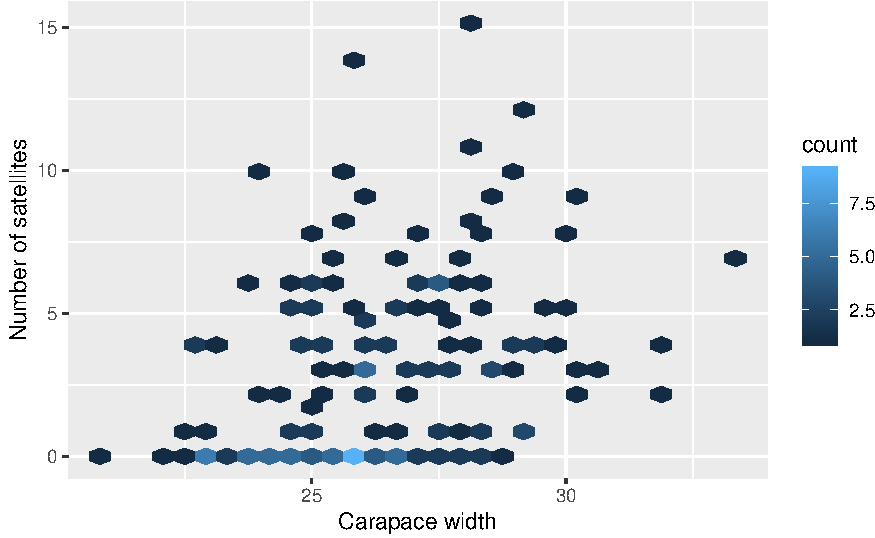
\includegraphics[width=0.7\linewidth]{_main_files/figure-latex/unnamed-chunk-25-1} \end{center}

\begin{itemize}
\tightlist
\item
  Large variability is observed.
\item
  Outlier: analysis with this observation and without it
\end{itemize}

For clarification,

\begin{Shaded}
\begin{Highlighting}[]
\NormalTok{(width_interval <-}
\StringTok{  }\NormalTok{crab }\OperatorTok
\StringTok{  }\KeywordTok{group_by}\NormalTok{(}\DataTypeTok{width =} \KeywordTok{cut}\NormalTok{(width,}
                       \DataTypeTok{breaks =} \KeywordTok{c}\NormalTok{(}\DecValTok{0}\NormalTok{, }\KeywordTok{seq}\NormalTok{(}\FloatTok{23.25}\NormalTok{, }\FloatTok{29.25}\NormalTok{, }\DataTypeTok{by =} \DecValTok{1}\NormalTok{), }\OtherTok{Inf}\NormalTok{),}
                       \DataTypeTok{ordered_result =} \OtherTok{TRUE}\NormalTok{)) }\OperatorTok
\StringTok{  }\KeywordTok{summarise}\NormalTok{(}\DataTypeTok{cases =} \KeywordTok{n}\NormalTok{(), }\DataTypeTok{S =} \KeywordTok{sum}\NormalTok{(sat), }\DataTypeTok{Mean =} \KeywordTok{mean}\NormalTok{(sat), }\DataTypeTok{Variance =} \KeywordTok{var}\NormalTok{(sat)))}
\end{Highlighting}
\end{Shaded}

\begin{verbatim}
# A tibble: 8 x 5
  width       cases     S  Mean Variance
  <ord>       <int> <dbl> <dbl>    <dbl>
1 (0,23.2]       14    14  1        2.77
2 (23.2,24.2]    14    20  1.43     8.88
3 (24.2,25.2]    28    67  2.39     6.54
4 (25.2,26.2]    39   105  2.69    11.4 
5 (26.2,27.2]    22    63  2.86     6.89
6 (27.2,28.2]    24    93  3.88     8.81
7 (28.2,29.2]    18    71  3.94    16.9 
8 (29.2,Inf]     14    72  5.14     8.29
\end{verbatim}

Looking at the table, we can see the \emph{nonlinear relationship} between sateliite counts and width.

\begin{Shaded}
\begin{Highlighting}[]
\NormalTok{crab }\OperatorTok
\StringTok{  }\KeywordTok{group_by}\NormalTok{(}\DataTypeTok{width =} \KeywordTok{cut}\NormalTok{(width,}
                       \DataTypeTok{breaks =} \KeywordTok{c}\NormalTok{(}\DecValTok{0}\NormalTok{, }\KeywordTok{seq}\NormalTok{(}\FloatTok{23.25}\NormalTok{, }\FloatTok{29.25}\NormalTok{, }\DataTypeTok{by =} \DecValTok{1}\NormalTok{), }\OtherTok{Inf}\NormalTok{),}
                       \DataTypeTok{ordered_result =} \OtherTok{TRUE}\NormalTok{)) }\OperatorTok
\StringTok{  }\KeywordTok{ggplot}\NormalTok{() }\OperatorTok{+}
\StringTok{  }\KeywordTok{aes}\NormalTok{(}\DataTypeTok{x =}\NormalTok{ width, }\DataTypeTok{y =}\NormalTok{ sat, }\DataTypeTok{fill =}\NormalTok{ width) }\OperatorTok{+}
\StringTok{  }\KeywordTok{geom_boxplot}\NormalTok{(}\DataTypeTok{show.legend =} \OtherTok{FALSE}\NormalTok{)}
\end{Highlighting}
\end{Shaded}

\begin{center}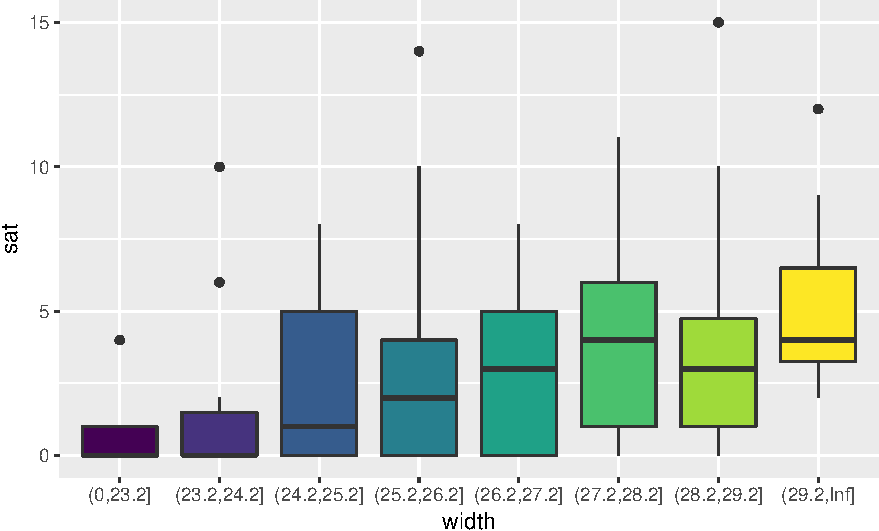
\includegraphics[width=0.7\linewidth]{_main_files/figure-latex/unnamed-chunk-27-1} \end{center}

\hypertarget{logistic-regression-model-2}{%
\subsection{Logistic regression model}\label{logistic-regression-model-2}}

Consider binary response

\[Y = \begin{cases} 1 & \text{if satellite}\: > 0 \\ 0 & \text{if satellite}\: = 0 \end{cases}\]

\begin{Shaded}
\begin{Highlighting}[]
\NormalTok{crab }\OperatorTok
\StringTok{  }\KeywordTok{select}\NormalTok{(y, width)}
\end{Highlighting}
\end{Shaded}

\begin{verbatim}
# A tibble: 173 x 2
       y width
   <dbl> <dbl>
 1     1  28.3
 2     0  22.5
 3     1  26  
 4     0  24.8
 5     1  26  
 6     0  23.8
 7     0  26.5
 8     0  24.7
 9     0  23.7
10     0  25.6
# ... with 163 more rows
\end{verbatim}

For \(\pi(x) = P(Y = 1) = \mu\),

\[\text{logit}\pi(x) \equiv \ln\frac{\pi(x)}{1 - \pi(x)} = \alpha + \beta x\]

\begin{Shaded}
\begin{Highlighting}[]
\NormalTok{logistic_fit <-}
\StringTok{  }\NormalTok{crab }\OperatorTok
\StringTok{  }\KeywordTok{glm}\NormalTok{(y }\OperatorTok{~}\StringTok{ }\NormalTok{width, }\DataTypeTok{family =} \KeywordTok{binomial}\NormalTok{(}\DataTypeTok{link =} \StringTok{"logit"}\NormalTok{), }\DataTypeTok{data =}\NormalTok{ .)}
\KeywordTok{summary}\NormalTok{(logistic_fit)}
\end{Highlighting}
\end{Shaded}

\begin{verbatim}

Call:
glm(formula = y ~ width, family = binomial(link = "logit"), data = .)

Deviance Residuals: 
   Min      1Q  Median      3Q     Max  
-2.028  -1.046   0.548   0.907   1.694  

Coefficients:
            Estimate Std. Error z value Pr(>|z|)    
(Intercept)  -12.351      2.629   -4.70  2.6e-06 ***
width          0.497      0.102    4.89  1.0e-06 ***
---
Signif. codes:  0 '***' 0.001 '**' 0.01 '*' 0.05 '.' 0.1 ' ' 1

(Dispersion parameter for binomial family taken to be 1)

    Null deviance: 225.76  on 172  degrees of freedom
Residual deviance: 194.45  on 171  degrees of freedom
AIC: 198.5

Number of Fisher Scoring iterations: 4
\end{verbatim}

Estimated odds of having satellites for each unit change in \texttt{width} is multiplied by

\[\frac{\hat\pi}{1 - \hat\pi} = \exp(\hat\beta) = 1.64\]

\hypertarget{poisson-regression}{%
\subsection{Poisson regression}\label{poisson-regression}}

Consider count response

\[Y = \text{the number of satellites} \sim Poisson(\mu)\]

\begin{Shaded}
\begin{Highlighting}[]
\NormalTok{crab }\OperatorTok
\StringTok{  }\KeywordTok{select}\NormalTok{(sat, width)}
\end{Highlighting}
\end{Shaded}

\begin{verbatim}
# A tibble: 173 x 2
     sat width
   <dbl> <dbl>
 1     8  28.3
 2     0  22.5
 3     9  26  
 4     0  24.8
 5     4  26  
 6     0  23.8
 7     0  26.5
 8     0  24.7
 9     0  23.7
10     0  25.6
# ... with 163 more rows
\end{verbatim}

\begin{Shaded}
\begin{Highlighting}[]
\NormalTok{pois_fit <-}
\StringTok{ }\NormalTok{crab }\OperatorTok
\StringTok{  }\KeywordTok{glm}\NormalTok{(sat }\OperatorTok{~}\StringTok{ }\NormalTok{width, }\DataTypeTok{data =}\NormalTok{ ., }\DataTypeTok{family =} \KeywordTok{poisson}\NormalTok{(}\DataTypeTok{link =} \StringTok{"log"}\NormalTok{))}
\KeywordTok{summary}\NormalTok{(pois_fit)}
\end{Highlighting}
\end{Shaded}

\begin{verbatim}

Call:
glm(formula = sat ~ width, family = poisson(link = "log"), data = .)

Deviance Residuals: 
   Min      1Q  Median      3Q     Max  
-2.853  -1.988  -0.493   1.097   4.922  

Coefficients:
            Estimate Std. Error z value Pr(>|z|)    
(Intercept)   -3.305      0.542   -6.09  1.1e-09 ***
width          0.164      0.020    8.22  < 2e-16 ***
---
Signif. codes:  0 '***' 0.001 '**' 0.01 '*' 0.05 '.' 0.1 ' ' 1

(Dispersion parameter for poisson family taken to be 1)

    Null deviance: 632.79  on 172  degrees of freedom
Residual deviance: 567.88  on 171  degrees of freedom
AIC: 927.2

Number of Fisher Scoring iterations: 6
\end{verbatim}

\hypertarget{goodness-of-fit}{%
\subsection{Goodness-of-fit}\label{goodness-of-fit}}

Deviance of \emph{exponential family} can be given by

\begin{equation}
\begin{split}
D(\mathbf{y}, \boldsymbol{\hat\mu}) & := -2(L_M - L_S) \\
& = LRT \quad\text{for}\: H_0: M \\
& = 2\sum_i\frac{y_i\tilde\theta_i - b(\tilde\theta_i)}{a(\phi)} - 2\sum_i\frac{y_i\hat\theta_i - b(\hat\theta_i)}{a(\phi)} \\
& \text{where}\quad \tilde\theta = \text{of saturated, and} \quad \hat\theta = \text{of the current model}
\end{split}
\end{equation}

For \(a(\phi) = \frac{\phi}{w_i}\), we compute \emph{scaled deviance}

\[\frac{D(\mathbf{y}, \boldsymbol{\hat\mu)}}{\phi} \approx \chi^2\]

It can be simplified in the Poisson GLM as

\[D(\mathbf{y}, \boldsymbol{\hat\mu}) = 2\sum_i\ln\frac{y_i}{\hat\mu_i}\]

To measure the goodness-of-fit, \textbf{analysis of deviance} can be conducted. Comparing two nested models with \(\phi = 1\), construct a test

\[M_0: \text{simpler model} \qquad\text{vs}\quad M_1: \text{complex model}\]

where \(M_0\) is \emph{nested within} \(M_1\). For each model, we can obtain scaled deviance written as

\[D_0 \equiv D(\mathbf{y}, \boldsymbol{\hat\mu_0}) \le D(\mathbf{y}, \boldsymbol{\hat\mu_1}) \equiv D_1\]

Then \emph{likelihood-ratio-test statistic} is applicable to the above test structure

\[G^2(M_0 \mid M_1) = D_0 - D_1 \stackrel{H_0}{\approx} \chi^2(\text{difference of parameters})\]

In case of canonical link GLMs,

\[G^2(M_0 \mid M_1) = 2\sum_i\hat\mu_{1i}\ln\frac{\hat\mu_{1i}}{\hat\mu_{0i}}\]

\begin{Shaded}
\begin{Highlighting}[]
\KeywordTok{anova}\NormalTok{(pois_fit, }\DataTypeTok{test =} \StringTok{"LRT"}\NormalTok{)}
\end{Highlighting}
\end{Shaded}

\begin{verbatim}
Analysis of Deviance Table

Model: poisson, link: log

Response: sat

Terms added sequentially (first to last)

      Df Deviance Resid. Df Resid. Dev Pr(>Chi)    
NULL                    172        633             
width  1     64.9       171        568  7.8e-16 ***
---
Signif. codes:  0 '***' 0.001 '**' 0.01 '*' 0.05 '.' 0.1 ' ' 1
\end{verbatim}

Here,

\[M_0: \text{null model} \qquad\text{vs}\quad M_1: \text{only width}\]

For this hypothesis, reject \(M_0\), i.e.~the fit of null model is poor compared to the current model. However, the size of residual deviance seems quite large while its degrees of freedom is only \texttt{1}.

\hypertarget{residual-analysis}{%
\subsection{Residual analysis}\label{residual-analysis}}

We now examine residual analysis. In general, \emph{standardized Pearson residual} is prefered.

\[r_i = \frac{y_i - \hat\mu_i}{\sqrt{V(\hat\mu_i)(1 - \hat{h}_i)}} = \frac{e_i}{\sqrt{V(\hat\mu_i)(1 - \hat{h}_i)}}\]

where \(\hat{h}_i\) is the hat values.

\begin{Shaded}
\begin{Highlighting}[]
\NormalTok{pois_resid <-}\StringTok{ }\KeywordTok{rstandard}\NormalTok{(pois_fit, }\DataTypeTok{type =} \StringTok{"pearson"}\NormalTok{)}
\KeywordTok{tibble}\NormalTok{(pois_resid) }\OperatorTok
\StringTok{  }\KeywordTok{ggplot}\NormalTok{(}\KeywordTok{aes}\NormalTok{(}\DataTypeTok{y =}\NormalTok{ pois_resid)) }\OperatorTok{+}
\StringTok{  }\KeywordTok{geom_boxplot}\NormalTok{() }\OperatorTok{+}
\StringTok{  }\KeywordTok{coord_flip}\NormalTok{()}
\end{Highlighting}
\end{Shaded}

\begin{center}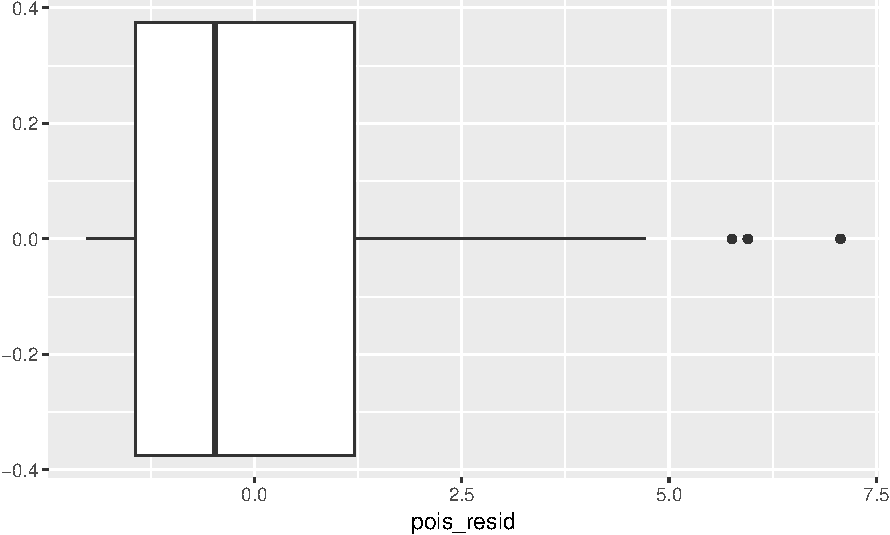
\includegraphics[width=0.7\linewidth]{_main_files/figure-latex/unnamed-chunk-33-1} \end{center}

Three large residuals can be observed.

\begin{Shaded}
\begin{Highlighting}[]
\KeywordTok{tibble}\NormalTok{(pois_resid) }\OperatorTok
\StringTok{  }\KeywordTok{ggplot}\NormalTok{() }\OperatorTok{+}
\StringTok{  }\KeywordTok{aes}\NormalTok{(}\DataTypeTok{sample =}\NormalTok{ pois_resid) }\OperatorTok{+}
\StringTok{  }\KeywordTok{geom_qq_line}\NormalTok{(}\DataTypeTok{col =} \StringTok{"grey"}\NormalTok{, }\DataTypeTok{size =} \FloatTok{1.5}\NormalTok{) }\OperatorTok{+}
\StringTok{  }\KeywordTok{geom_qq}\NormalTok{()}
\end{Highlighting}
\end{Shaded}

\begin{center}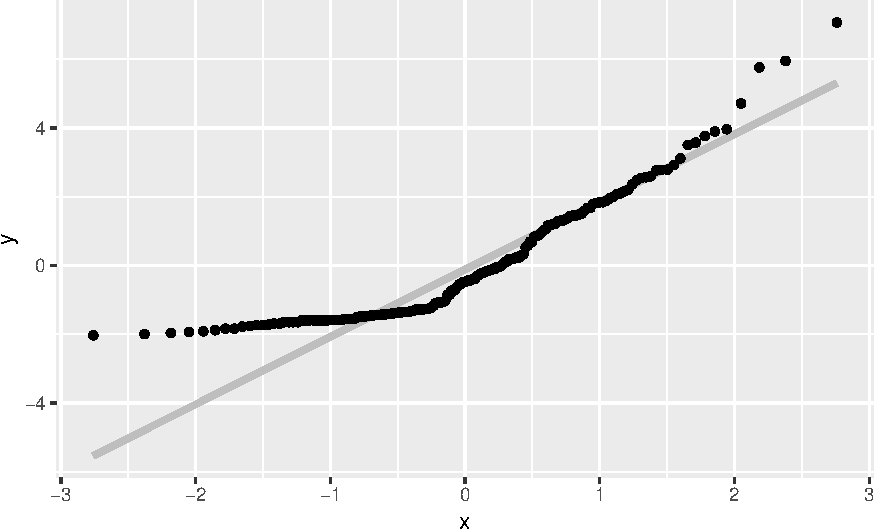
\includegraphics[width=0.7\linewidth]{_main_files/figure-latex/unnamed-chunk-34-1} \end{center}

\begin{Shaded}
\begin{Highlighting}[]
\KeywordTok{data_frame}\NormalTok{(}\DataTypeTok{pred =} \KeywordTok{predict}\NormalTok{(pois_fit, }\DataTypeTok{type =} \StringTok{"response"}\NormalTok{),}
         \DataTypeTok{resid =}\NormalTok{ pois_resid) }\OperatorTok
\StringTok{  }\KeywordTok{ggplot}\NormalTok{() }\OperatorTok{+}
\StringTok{  }\KeywordTok{aes}\NormalTok{(pred, resid) }\OperatorTok{+}
\StringTok{  }\KeywordTok{geom_hline}\NormalTok{(}\DataTypeTok{yintercept =} \DecValTok{0}\NormalTok{, }\DataTypeTok{alpha =} \FloatTok{.5}\NormalTok{) }\OperatorTok{+}
\StringTok{  }\KeywordTok{geom_jitter}\NormalTok{() }\OperatorTok{+}
\StringTok{  }\KeywordTok{geom_vline}\NormalTok{(}\DataTypeTok{xintercept =} \DecValTok{5}\NormalTok{, }\DataTypeTok{col =} \StringTok{"red"}\NormalTok{) }\OperatorTok{+}
\StringTok{  }\KeywordTok{geom_hline}\NormalTok{(}\DataTypeTok{yintercept =} \DecValTok{5}\NormalTok{, }\DataTypeTok{col =} \StringTok{"red"}\NormalTok{)}
\end{Highlighting}
\end{Shaded}

\begin{center}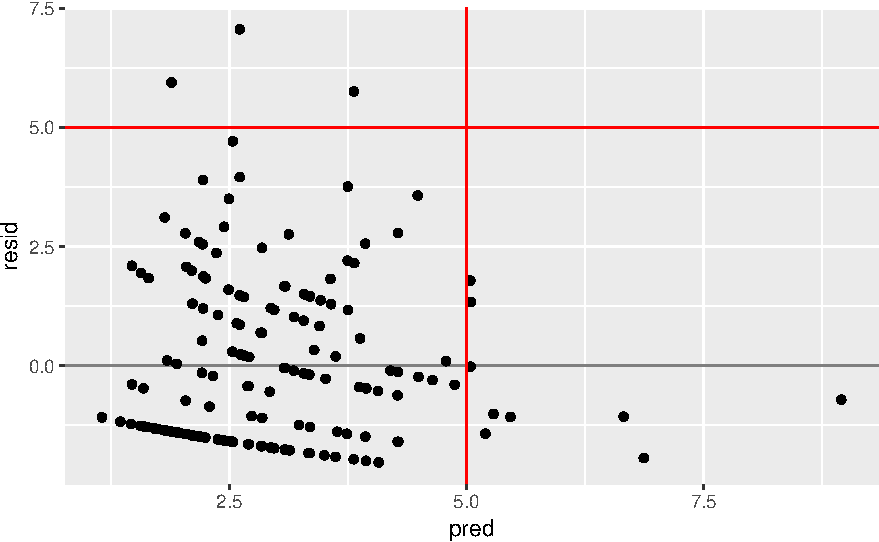
\includegraphics[width=0.7\linewidth]{_main_files/figure-latex/unnamed-chunk-35-1} \end{center}

The set of \(r_i\) seems variable. It cannot be said to be a good fit.

\hypertarget{overdispersion-for-poisson-glms}{%
\subsection{Overdispersion for Poisson GLMs}\label{overdispersion-for-poisson-glms}}

\begin{Shaded}
\begin{Highlighting}[]
\NormalTok{width_interval}
\end{Highlighting}
\end{Shaded}

\begin{verbatim}
# A tibble: 8 x 5
  width       cases     S  Mean Variance
  <ord>       <int> <dbl> <dbl>    <dbl>
1 (0,23.2]       14    14  1        2.77
2 (23.2,24.2]    14    20  1.43     8.88
3 (24.2,25.2]    28    67  2.39     6.54
4 (25.2,26.2]    39   105  2.69    11.4 
5 (26.2,27.2]    22    63  2.86     6.89
6 (27.2,28.2]    24    93  3.88     8.81
7 (28.2,29.2]    18    71  3.94    16.9 
8 (29.2,Inf]     14    72  5.14     8.29
\end{verbatim}

Theoretically, for Poisson distribution,

\[E(Y) = Var(Y) = \mu\]

However as we can see, sample variance(\texttt{Variance}) is much larger than sample mean(\texttt{Mean}). In this data set, \texttt{width} is not the only predictor that affects the response. Not only that, but also \texttt{weight}, \texttt{color}, and \texttt{spine} can be in the systematic component. Thus, \(\mu\) is varied for each combination of \((\text{width, weight, color, spine})^T = \mathbf{x}\). We now have \emph{conditional distribution}

\[Y \mid \mu \sim Poisson(\mu)\]

which gives

\[E(Y \mid \mu) = Var(Y \mid \mu) = \mu\]

Let

\[\theta := E(\mu)\]

Then

\[E(Y) = E\big[E(Y \mid \mu)\big] = E(\mu) = \theta\]

and

\[Var(Y) = E\big[ Var(Y \mid \mu) \big] + Var\big[ E(Y \mid \mu) \big] = E(\mu) + Var(\mu) > \theta\]

Hence,

\[Var(Y) > E(Y)\]

\hypertarget{negative-binomial-glms}{%
\subsection{Negative Binomial GLMs}\label{negative-binomial-glms}}

Negative binomial distribution which also takes into account count response can be a good candidates. Let \(Y\) be the negative binomial random variable with parameters \(\mu\) and \(\gamma = \frac{1}{k}\). Then

\[E(Y) = \mu \quad < Var(Y) = \mu + \gamma\mu^2\]

Here, \(\gamma > 0\) is called \emph{dispersion parameter}. \texttt{MASS} library enables to fit the negative binomial random component and corresponding link functions. There are two ways to fit this random component.

\begin{itemize}
\tightlist
\item
  \texttt{MASS::glm.nb()} itself performs what we want, by default \texttt{link\ =\ log}

  \begin{itemize}
  \tightlist
  \item
    link function must be specified among: \texttt{log}, \texttt{sqrt}, or \texttt{identity}
  \item
    \texttt{init.theta} = dispersion parameter is optional: if omitted, moment estimator by Poisson GLM is used
  \end{itemize}
\item
  Specify \texttt{family} option by \texttt{MASS::negative.binomial(theta,\ link)} of base \texttt{glm()}

  \begin{itemize}
  \tightlist
  \item
    \emph{dispersion parameter} \texttt{theta} must be chosen
  \end{itemize}
\end{itemize}

\begin{Shaded}
\begin{Highlighting}[]
\NormalTok{crab }\OperatorTok
\StringTok{  }\NormalTok{MASS}\OperatorTok{::}\KeywordTok{glm.nb}\NormalTok{(sat }\OperatorTok{~}\StringTok{ }\NormalTok{width, }\DataTypeTok{data =}\NormalTok{ .,}
               \DataTypeTok{link =}\NormalTok{ identity,}
               \DataTypeTok{mustart =} \KeywordTok{predict}\NormalTok{(pois_fit, }\DataTypeTok{type =} \StringTok{"response"}\NormalTok{))}
\end{Highlighting}
\end{Shaded}

\begin{verbatim}

Call:  MASS::glm.nb(formula = sat ~ width, data = ., mustart = predict(pois_fit, 
    type = "response"), link = identity, init.theta = 0.9316967133)

Coefficients:
(Intercept)        width  
    -11.634        0.554  

Degrees of Freedom: 172 Total (i.e. Null);  171 Residual
Null Deviance:      217 
Residual Deviance: 196  AIC: 754
\end{verbatim}

\begin{Shaded}
\begin{Highlighting}[]
\NormalTok{crab }\OperatorTok
\StringTok{  }\KeywordTok{glm}\NormalTok{(sat }\OperatorTok{~}\StringTok{ }\NormalTok{width, }\DataTypeTok{data =}\NormalTok{ .,}
      \DataTypeTok{family =}\NormalTok{ MASS}\OperatorTok{::}\KeywordTok{negative.binomial}\NormalTok{(}\DataTypeTok{theta =} \FloatTok{.9}\NormalTok{, }\DataTypeTok{link =} \StringTok{"identity"}\NormalTok{),}
      \DataTypeTok{start =} \KeywordTok{coef}\NormalTok{(pois_fit))}
\end{Highlighting}
\end{Shaded}

\begin{verbatim}

Call:  glm(formula = sat ~ width, family = MASS::negative.binomial(theta = 0.9, 
    link = "identity"), data = ., start = coef(pois_fit))

Coefficients:
(Intercept)        width  
    -11.634        0.554  

Degrees of Freedom: 172 Total (i.e. Null);  171 Residual
Null Deviance:      212 
Residual Deviance: 192  AIC: 752
\end{verbatim}

We now implement \texttt{log} link which is more typically used.

\begin{Shaded}
\begin{Highlighting}[]
\NormalTok{neg_fit <-}
\StringTok{  }\NormalTok{crab }\OperatorTok
\StringTok{  }\KeywordTok{glm}\NormalTok{(sat }\OperatorTok{~}\StringTok{ }\NormalTok{width, }\DataTypeTok{data =}\NormalTok{ .,}
      \DataTypeTok{family =}\NormalTok{ MASS}\OperatorTok{::}\KeywordTok{negative.binomial}\NormalTok{(}\DataTypeTok{theta =} \FloatTok{.9}\NormalTok{, }\DataTypeTok{link =} \StringTok{"log"}\NormalTok{))}
\KeywordTok{summary}\NormalTok{(neg_fit)}
\end{Highlighting}
\end{Shaded}

\begin{verbatim}

Call:
glm(formula = sat ~ width, family = MASS::negative.binomial(theta = 0.9, 
    link = "log"), data = .)

Deviance Residuals: 
   Min      1Q  Median      3Q     Max  
-1.778  -1.410  -0.250   0.476   2.014  

Coefficients:
            Estimate Std. Error t value Pr(>|t|)    
(Intercept)  -4.0534     1.0779   -3.76  0.00023 ***
width         0.1921     0.0405    4.74  4.5e-06 ***
---
Signif. codes:  0 '***' 0.001 '**' 0.01 '*' 0.05 '.' 0.1 ' ' 1

(Dispersion parameter for Negative Binomial(0.9) family taken to be 0.843)

    Null deviance: 212.46  on 172  degrees of freedom
Residual deviance: 195.28  on 171  degrees of freedom
AIC: 755.3

Number of Fisher Scoring iterations: 5
\end{verbatim}

\begin{Shaded}
\begin{Highlighting}[]
\KeywordTok{anova}\NormalTok{(neg_fit, }\DataTypeTok{test =} \StringTok{"LRT"}\NormalTok{)}
\end{Highlighting}
\end{Shaded}

\begin{verbatim}
Analysis of Deviance Table

Model: Negative Binomial(0.9), link: log

Response: sat

Terms added sequentially (first to last)

      Df Deviance Resid. Df Resid. Dev Pr(>Chi)    
NULL                    172        212             
width  1     17.2       171        195  6.4e-06 ***
---
Signif. codes:  0 '***' 0.001 '**' 0.01 '*' 0.05 '.' 0.1 ' ' 1
\end{verbatim}

Residual deviance is much smaller than poisson regression.

\begin{Shaded}
\begin{Highlighting}[]
\NormalTok{neg_resid <-}\StringTok{ }\KeywordTok{rstandard}\NormalTok{(neg_fit, }\DataTypeTok{type =} \StringTok{"pearson"}\NormalTok{)}
\KeywordTok{tibble}\NormalTok{(neg_resid) }\OperatorTok
\StringTok{  }\KeywordTok{ggplot}\NormalTok{(}\KeywordTok{aes}\NormalTok{(}\DataTypeTok{y =}\NormalTok{ neg_resid)) }\OperatorTok{+}
\StringTok{  }\KeywordTok{geom_boxplot}\NormalTok{() }\OperatorTok{+}
\StringTok{  }\KeywordTok{coord_flip}\NormalTok{()}
\end{Highlighting}
\end{Shaded}

\begin{center}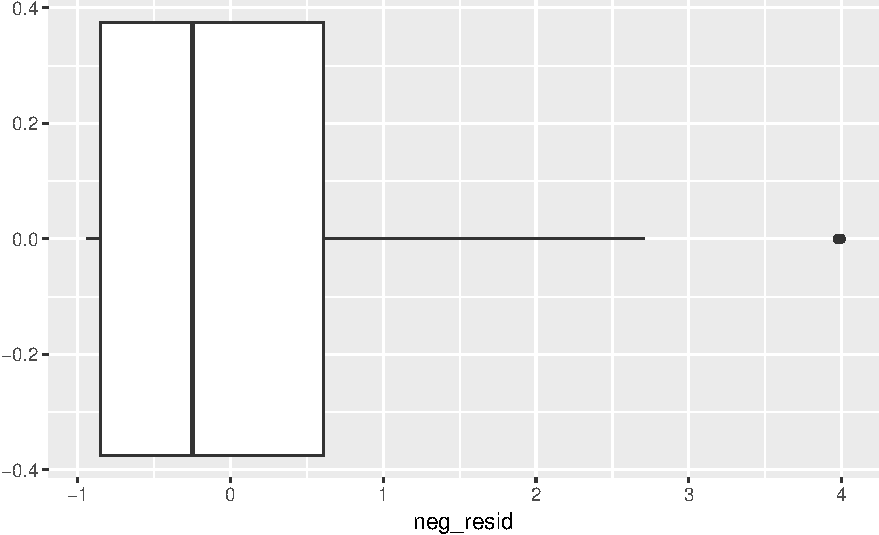
\includegraphics[width=0.7\linewidth]{_main_files/figure-latex/unnamed-chunk-41-1} \end{center}

Standardized residuals are not large.

\begin{Shaded}
\begin{Highlighting}[]
\KeywordTok{tibble}\NormalTok{(neg_resid) }\OperatorTok
\StringTok{  }\KeywordTok{ggplot}\NormalTok{() }\OperatorTok{+}
\StringTok{  }\KeywordTok{aes}\NormalTok{(}\DataTypeTok{sample =}\NormalTok{ neg_resid) }\OperatorTok{+}
\StringTok{  }\KeywordTok{geom_qq_line}\NormalTok{(}\DataTypeTok{col =} \StringTok{"grey"}\NormalTok{, }\DataTypeTok{size =} \FloatTok{1.5}\NormalTok{) }\OperatorTok{+}
\StringTok{  }\KeywordTok{geom_qq}\NormalTok{()}
\end{Highlighting}
\end{Shaded}

\begin{center}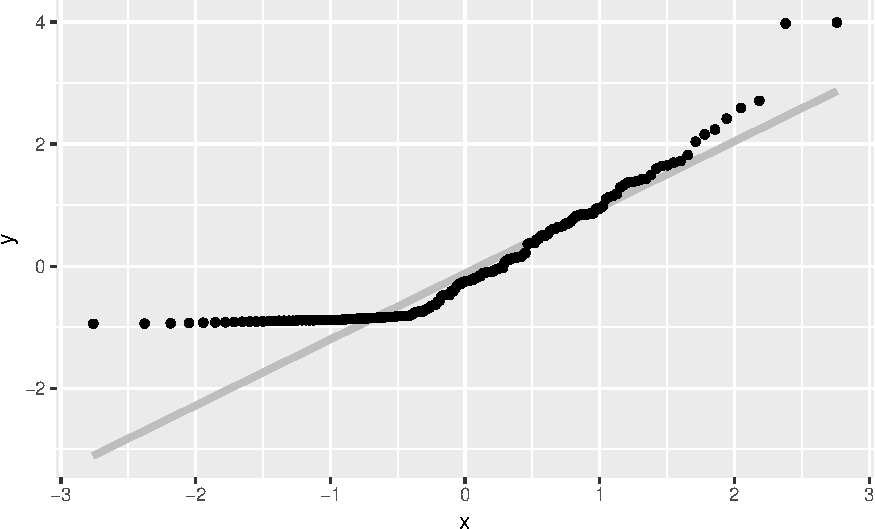
\includegraphics[width=0.7\linewidth]{_main_files/figure-latex/unnamed-chunk-42-1} \end{center}

\begin{Shaded}
\begin{Highlighting}[]
\KeywordTok{data_frame}\NormalTok{(}\DataTypeTok{pred =} \KeywordTok{predict}\NormalTok{(neg_fit, }\DataTypeTok{type =} \StringTok{"response"}\NormalTok{),}
         \DataTypeTok{resid =}\NormalTok{ neg_resid) }\OperatorTok
\StringTok{  }\KeywordTok{ggplot}\NormalTok{() }\OperatorTok{+}
\StringTok{  }\KeywordTok{aes}\NormalTok{(pred, resid) }\OperatorTok{+}
\StringTok{  }\KeywordTok{geom_hline}\NormalTok{(}\DataTypeTok{yintercept =} \DecValTok{0}\NormalTok{, }\DataTypeTok{alpha =} \FloatTok{.5}\NormalTok{) }\OperatorTok{+}
\StringTok{  }\KeywordTok{geom_jitter}\NormalTok{() }\OperatorTok{+}
\StringTok{  }\KeywordTok{geom_vline}\NormalTok{(}\DataTypeTok{xintercept =} \DecValTok{5}\NormalTok{, }\DataTypeTok{col =} \StringTok{"red"}\NormalTok{) }\OperatorTok{+}
\StringTok{  }\KeywordTok{geom_hline}\NormalTok{(}\DataTypeTok{yintercept =} \DecValTok{3}\NormalTok{, }\DataTypeTok{col =} \StringTok{"red"}\NormalTok{)}
\end{Highlighting}
\end{Shaded}

\begin{center}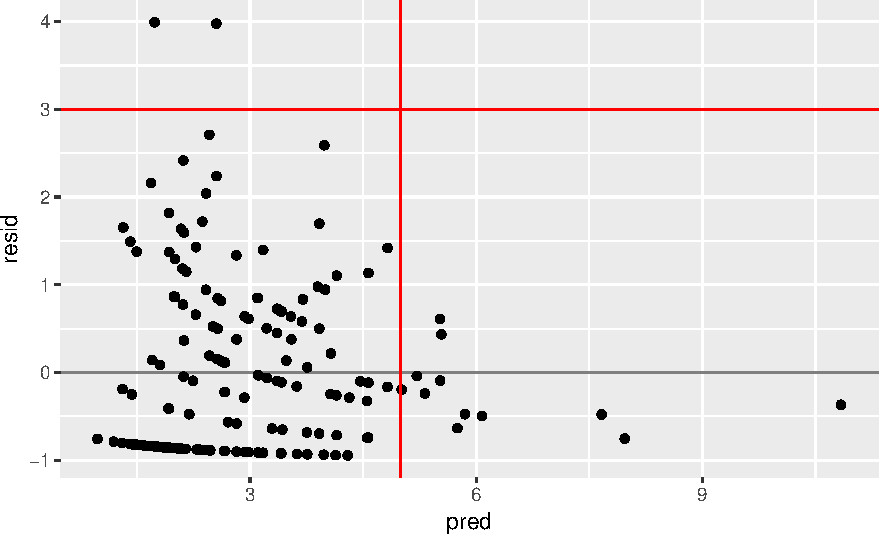
\includegraphics[width=0.7\linewidth]{_main_files/figure-latex/unnamed-chunk-43-1} \end{center}

Compared to the poisson regression model, this model results in less variable residuals.

\hypertarget{logistic-regression}{%
\chapter{Logistic Regression}\label{logistic-regression}}

\begin{Shaded}
\begin{Highlighting}[]
\KeywordTok{library}\NormalTok{(tidyverse)}
\CommentTok{# library(knitr)}
\CommentTok{# library(kableExtra)}
\CommentTok{# library(formattable)}
\end{Highlighting}
\end{Shaded}

\hypertarget{horseshoe-crab-data}{%
\section{Horseshoe crab data}\label{horseshoe-crab-data}}

\begin{Shaded}
\begin{Highlighting}[]
\NormalTok{(crab <-}\StringTok{ }\KeywordTok{read_table}\NormalTok{(}\StringTok{"data/Crabs.dat"}\NormalTok{))}
\end{Highlighting}
\end{Shaded}

\begin{verbatim}
# A tibble: 173 x 7
    crab   sat     y weight width color spine
   <dbl> <dbl> <dbl>  <dbl> <dbl> <dbl> <dbl>
 1     1     8     1   3.05  28.3     2     3
 2     2     0     0   1.55  22.5     3     3
 3     3     9     1   2.3   26       1     1
 4     4     0     0   2.1   24.8     3     3
 5     5     4     1   2.6   26       3     3
 6     6     0     0   2.1   23.8     2     3
 7     7     0     0   2.35  26.5     1     1
 8     8     0     0   1.9   24.7     3     2
 9     9     0     0   1.95  23.7     2     1
10    10     0     0   2.15  25.6     3     3
# ... with 163 more rows
\end{verbatim}

\begin{Shaded}
\begin{Highlighting}[]
\NormalTok{crab }\OperatorTok\StringTok{ }
\StringTok{  }\KeywordTok{mutate}\NormalTok{(}
    \DataTypeTok{sat =} \KeywordTok{color_tile}\NormalTok{(}\StringTok{"white"}\NormalTok{, }\StringTok{"red"}\NormalTok{)(sat),}
    \DataTypeTok{y =} \KeywordTok{color_tile}\NormalTok{(}\StringTok{"white"}\NormalTok{, }\StringTok{"red"}\NormalTok{)(y),}
    \DataTypeTok{weight =} \KeywordTok{color_bar}\NormalTok{(}\StringTok{"lightblue"}\NormalTok{)(weight),}
    \DataTypeTok{width =} \KeywordTok{color_bar}\NormalTok{(}\StringTok{"lightgreen"}\NormalTok{)(width),}
    \DataTypeTok{color =} \KeywordTok{cell_spec}\NormalTok{(}
\NormalTok{      color,}
      \DataTypeTok{color =} \KeywordTok{spec_color}\NormalTok{(color, }\DataTypeTok{direction =} \DecValTok{-1}\NormalTok{)}
\NormalTok{    ),}
    \DataTypeTok{spine =} \KeywordTok{cell_spec}\NormalTok{(}
\NormalTok{      spine,}
      \DataTypeTok{color =} \KeywordTok{spec_color}\NormalTok{(spine)}
\NormalTok{    )}
\NormalTok{  ) }\OperatorTok\StringTok{ }
\StringTok{  }\KeywordTok{head}\NormalTok{() }\OperatorTok\StringTok{ }
\StringTok{  }\KeywordTok{kable}\NormalTok{(}\DataTypeTok{format =} \StringTok{"latex"}\NormalTok{, }\DataTypeTok{escape =} \OtherTok{FALSE}\NormalTok{,}
        \DataTypeTok{col.names =} \KeywordTok{c}\NormalTok{(}\StringTok{"crab"}\NormalTok{, }\StringTok{"Satellites"}\NormalTok{, }\StringTok{"y"}\NormalTok{, }\StringTok{"Weight(kg)"}\NormalTok{, }\StringTok{"carapace width(cm)"}\NormalTok{, }\StringTok{"Color"}\NormalTok{, }\StringTok{"spine condition"}\NormalTok{)) }\OperatorTok\StringTok{ }
\StringTok{  }\KeywordTok{kable_styling}\NormalTok{(}\StringTok{"hover"}\NormalTok{)}
\end{Highlighting}
\end{Shaded}

\[y_i = \begin{cases} 1 & \text{crab}\: i \:\text{has at least one satellite} \\ 0 & \text{crab}\: i \:\text{does not have satellite} \end{cases}\]

\begin{quote}
Does the female crab's carapace width is related to this binary response?
\end{quote}

Looking at the above data set in the eye, large width can help the crab have satellites. Let's check it out.

\begin{Shaded}
\begin{Highlighting}[]
\NormalTok{crab }\OperatorTok\StringTok{ }
\StringTok{  }\KeywordTok{ggplot}\NormalTok{() }\OperatorTok{+}
\StringTok{  }\KeywordTok{aes}\NormalTok{(width, sat) }\OperatorTok{+}
\StringTok{  }\KeywordTok{geom_hex}\NormalTok{() }\OperatorTok{+}
\StringTok{  }\KeywordTok{labs}\NormalTok{(}
    \DataTypeTok{x =} \StringTok{"Width"}\NormalTok{,}
    \DataTypeTok{y =} \StringTok{"Number of Satellite"}
\NormalTok{  )}
\end{Highlighting}
\end{Shaded}

\begin{figure}[H]

{\centering 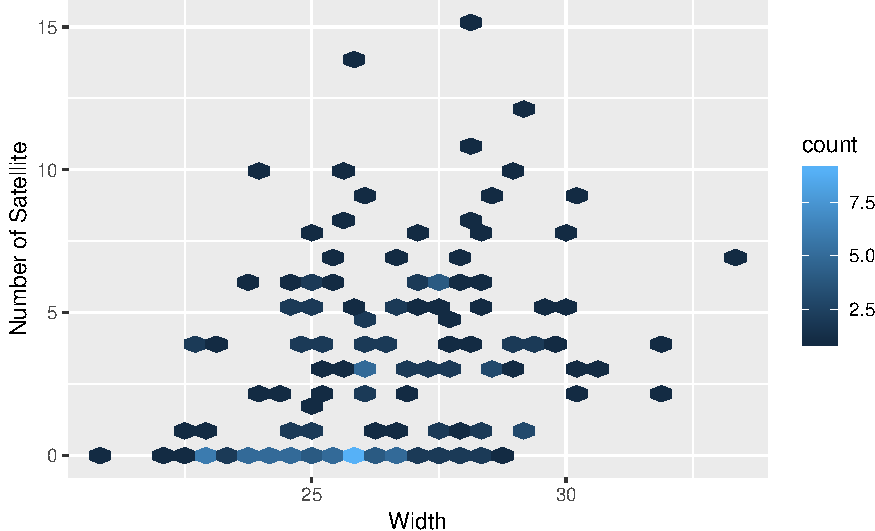
\includegraphics[width=0.7\linewidth]{_main_files/figure-latex/crabscat-1} 

}

\caption{Number of satellites by width of female crab\label{crabscat}}\label{fig:crabscat}
\end{figure}

large variability.

\begin{Shaded}
\begin{Highlighting}[]
\NormalTok{crab }\OperatorTok\StringTok{ }
\StringTok{  }\KeywordTok{group_by}\NormalTok{(}\DataTypeTok{width_cut =} \KeywordTok{cut}\NormalTok{(width, }\DecValTok{8}\NormalTok{, }\DataTypeTok{ordered_result =} \OtherTok{TRUE}\NormalTok{)) }\OperatorTok
\StringTok{  }\KeywordTok{ggplot}\NormalTok{() }\OperatorTok{+}
\StringTok{  }\KeywordTok{aes}\NormalTok{(width_cut, sat) }\OperatorTok{+}
\StringTok{  }\KeywordTok{geom_boxplot}\NormalTok{() }\OperatorTok{+}
\StringTok{  }\KeywordTok{labs}\NormalTok{(}
    \DataTypeTok{x =} \StringTok{"Levels of width"}\NormalTok{,}
    \DataTypeTok{y =} \StringTok{"Number of Satellite"}
\NormalTok{  )}
\end{Highlighting}
\end{Shaded}

\begin{figure}[H]

{\centering 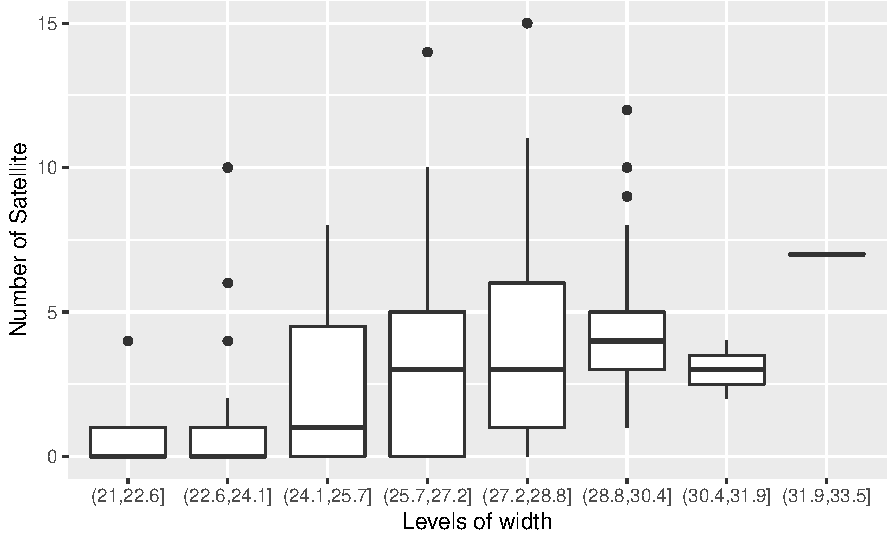
\includegraphics[width=0.7\linewidth]{_main_files/figure-latex/crabdist-1} 

}

\caption{Distribution of satellites by width of female crab\label{crabdist}}\label{fig:crabdist}
\end{figure}

\hypertarget{inference-for-logistic-regression}{%
\section{Inference for logistic regression}\label{inference-for-logistic-regression}}

\[logit[\pi(x)] = \alpha + \beta x\]

\begin{Shaded}
\begin{Highlighting}[]
\NormalTok{(width_fit <-}
\StringTok{  }\NormalTok{crab }\OperatorTok\StringTok{ }
\StringTok{  }\KeywordTok{select}\NormalTok{(y, width) }\OperatorTok\StringTok{ }
\StringTok{  }\KeywordTok{glm}\NormalTok{(y }\OperatorTok{~}\StringTok{ }\NormalTok{., }\DataTypeTok{data =}\NormalTok{ ., }\DataTypeTok{family =} \KeywordTok{binomial}\NormalTok{())) }\OperatorTok\StringTok{ }
\StringTok{  }\KeywordTok{summary}\NormalTok{()}
\end{Highlighting}
\end{Shaded}

\begin{verbatim}

Call:
glm(formula = y ~ ., family = binomial(), data = .)

Deviance Residuals: 
   Min      1Q  Median      3Q     Max  
-2.028  -1.046   0.548   0.907   1.694  

Coefficients:
            Estimate Std. Error z value Pr(>|z|)    
(Intercept)  -12.351      2.629   -4.70  2.6e-06 ***
width          0.497      0.102    4.89  1.0e-06 ***
---
Signif. codes:  0 '***' 0.001 '**' 0.01 '*' 0.05 '.' 0.1 ' ' 1

(Dispersion parameter for binomial family taken to be 1)

    Null deviance: 225.76  on 172  degrees of freedom
Residual deviance: 194.45  on 171  degrees of freedom
AIC: 198.5

Number of Fisher Scoring iterations: 4
\end{verbatim}

\hypertarget{wald-test}{%
\subsection{Wald test}\label{wald-test}}

\[Z = \frac{\hat\beta - \beta_0}{SE} \stackrel{H_0}{\approx} N(0, 1)\]

Equivalently,

\[Z^2 \stackrel{H_0}{\approx} \chi^2_1\]

If multivariate,

\[W = (\boldsymbol{\hat\beta} - \boldsymbol\beta)^T\Big[Cov(\boldsymbol{\hat\beta})\Big]^{-1}(\boldsymbol{\hat\beta} - \boldsymbol\beta) \stackrel{H_0}{\approx} \chi^2_p\]

\begin{Shaded}
\begin{Highlighting}[]
\NormalTok{broom}\OperatorTok{::}\KeywordTok{tidy}\NormalTok{(width_fit) }\OperatorTok\StringTok{ }
\StringTok{  }\KeywordTok{bind_cols}\NormalTok{(broom}\OperatorTok{::}\KeywordTok{confint_tidy}\NormalTok{(width_fit)) }\OperatorTok\StringTok{ }
\StringTok{  }\NormalTok{pander}\OperatorTok{::}\KeywordTok{pander}\NormalTok{()}
\end{Highlighting}
\end{Shaded}

\begin{longtable}[]{@{}ccccccc@{}}
\toprule
\begin{minipage}[b]{0.13\columnwidth}\centering
term\strut
\end{minipage} & \begin{minipage}[b]{0.11\columnwidth}\centering
estimate\strut
\end{minipage} & \begin{minipage}[b]{0.12\columnwidth}\centering
std.error\strut
\end{minipage} & \begin{minipage}[b]{0.12\columnwidth}\centering
statistic\strut
\end{minipage} & \begin{minipage}[b]{0.12\columnwidth}\centering
p.value\strut
\end{minipage} & \begin{minipage}[b]{0.11\columnwidth}\centering
conf.low\strut
\end{minipage} & \begin{minipage}[b]{0.12\columnwidth}\centering
conf.high\strut
\end{minipage}\tabularnewline
\midrule
\endhead
\begin{minipage}[t]{0.13\columnwidth}\centering
(Intercept)\strut
\end{minipage} & \begin{minipage}[t]{0.11\columnwidth}\centering
-12.35\strut
\end{minipage} & \begin{minipage}[t]{0.12\columnwidth}\centering
2.629\strut
\end{minipage} & \begin{minipage}[t]{0.12\columnwidth}\centering
-4.698\strut
\end{minipage} & \begin{minipage}[t]{0.12\columnwidth}\centering
2.622e-06\strut
\end{minipage} & \begin{minipage}[t]{0.11\columnwidth}\centering
-17.81\strut
\end{minipage} & \begin{minipage}[t]{0.12\columnwidth}\centering
-7.457\strut
\end{minipage}\tabularnewline
\begin{minipage}[t]{0.13\columnwidth}\centering
width\strut
\end{minipage} & \begin{minipage}[t]{0.11\columnwidth}\centering
0.4972\strut
\end{minipage} & \begin{minipage}[t]{0.12\columnwidth}\centering
0.1017\strut
\end{minipage} & \begin{minipage}[t]{0.12\columnwidth}\centering
4.887\strut
\end{minipage} & \begin{minipage}[t]{0.12\columnwidth}\centering
1.021e-06\strut
\end{minipage} & \begin{minipage}[t]{0.11\columnwidth}\centering
0.3084\strut
\end{minipage} & \begin{minipage}[t]{0.12\columnwidth}\centering
0.709\strut
\end{minipage}\tabularnewline
\bottomrule
\end{longtable}

\hypertarget{likelihood-ratio-test}{%
\subsection{Likelihood ratio test}\label{likelihood-ratio-test}}

\[G^2 = -2(L_0 - L_1)\]

\begin{Shaded}
\begin{Highlighting}[]
\NormalTok{(width_lr <-}\StringTok{ }\KeywordTok{anova}\NormalTok{(width_fit, }\DataTypeTok{test =} \StringTok{"LRT"}\NormalTok{))}
\end{Highlighting}
\end{Shaded}

\begin{verbatim}
Analysis of Deviance Table

Model: binomial, link: logit

Response: y

Terms added sequentially (first to last)

      Df Deviance Resid. Df Resid. Dev Pr(>Chi)    
NULL                    172        226             
width  1     31.3       171        194  2.2e-08 ***
---
Signif. codes:  0 '***' 0.001 '**' 0.01 '*' 0.05 '.' 0.1 ' ' 1
\end{verbatim}

\hypertarget{score-test}{%
\subsection{Score test}\label{score-test}}

With dispersion of 1, we have

\[Var(Y_i) = V(\mu_i)\]

and so

\[X^2 = \sum_{i = 1}^n\frac{(y_i - \hat\mu_i)^2}{V(\hat\mu_i)}\]

\begin{Shaded}
\begin{Highlighting}[]
\NormalTok{(width_sc <-}\StringTok{ }\KeywordTok{anova}\NormalTok{(width_fit, }\DataTypeTok{test =} \StringTok{"Rao"}\NormalTok{))}
\end{Highlighting}
\end{Shaded}

\begin{verbatim}
Analysis of Deviance Table

Model: binomial, link: logit

Response: y

Terms added sequentially (first to last)

      Df Deviance Resid. Df Resid. Dev  Rao Pr(>Chi)    
NULL                    172        226                  
width  1     31.3       171        194 27.9  1.3e-07 ***
---
Signif. codes:  0 '***' 0.001 '**' 0.01 '*' 0.05 '.' 0.1 ' ' 1
\end{verbatim}

In sum,

\begin{longtable}[]{@{}cccc@{}}
\toprule
\begin{minipage}[b]{0.10\columnwidth}\centering
Test\strut
\end{minipage} & \begin{minipage}[b]{0.16\columnwidth}\centering
Chi-Square\strut
\end{minipage} & \begin{minipage}[b]{0.06\columnwidth}\centering
DF\strut
\end{minipage} & \begin{minipage}[b]{0.16\columnwidth}\centering
Pr \textgreater{} ChiSq\strut
\end{minipage}\tabularnewline
\midrule
\endhead
\begin{minipage}[t]{0.10\columnwidth}\centering
LRT\strut
\end{minipage} & \begin{minipage}[t]{0.16\columnwidth}\centering
31.31\strut
\end{minipage} & \begin{minipage}[t]{0.06\columnwidth}\centering
1\strut
\end{minipage} & \begin{minipage}[t]{0.16\columnwidth}\centering
2.204e-08\strut
\end{minipage}\tabularnewline
\begin{minipage}[t]{0.10\columnwidth}\centering
Score\strut
\end{minipage} & \begin{minipage}[t]{0.16\columnwidth}\centering
27.88\strut
\end{minipage} & \begin{minipage}[t]{0.06\columnwidth}\centering
1\strut
\end{minipage} & \begin{minipage}[t]{0.16\columnwidth}\centering
1.294e-07\strut
\end{minipage}\tabularnewline
\bottomrule
\end{longtable}

\hypertarget{confidence-interval-for-logit}{%
\subsection{Confidence interval for logit}\label{confidence-interval-for-logit}}

\(Cov(\boldsymbol{\hat\beta})\) is given as

\begin{Shaded}
\begin{Highlighting}[]
\KeywordTok{vcov}\NormalTok{(width_fit)}
\end{Highlighting}
\end{Shaded}

\begin{verbatim}
            (Intercept)   width
(Intercept)       6.910 -0.2668
width            -0.267  0.0104
\end{verbatim}

Then

\[Cov(\hat\alpha + \hat\beta x_0) = \left[\begin{array}{cc} 1 & x_0 \end{array}\right] Cov(\boldsymbol{\hat\beta})\left[\begin{array}{c} 1 \\ x_0 \end{array}\right] = Var(\hat\alpha) + x_0^2Var(\hat\beta) + 2x_0Cov(\hat\alpha, \hat\beta)\]

For \(x_0 = 26.5\), for instance,

\begin{Shaded}
\begin{Highlighting}[]
\NormalTok{x0 <-}\StringTok{ }\KeywordTok{c}\NormalTok{(}\DecValTok{1}\NormalTok{, }\FloatTok{26.5}\NormalTok{)}
\KeywordTok{t}\NormalTok{(x0) }\OperatorTok\StringTok{ }\KeywordTok{vcov}\NormalTok{(width_fit) }\OperatorTok\StringTok{ }\NormalTok{x0}
\end{Highlighting}
\end{Shaded}

\begin{verbatim}
       [,1]
[1,] 0.0356
\end{verbatim}

Then we can calculate

\[(\hat\alpha + \hat\beta x_0) + z_{\frac{\alpha}{2}} SE\]

On the other hand, \texttt{predict.glm(se.fit\ =\ TRUE)} gives above value in \texttt{\$se.fit} as \emph{standard error}, i.e.~squared value.

\begin{Shaded}
\begin{Highlighting}[]
\KeywordTok{data_frame}\NormalTok{(}\DataTypeTok{width =} \FloatTok{26.5}\NormalTok{) }\OperatorTok\StringTok{ }
\StringTok{  }\KeywordTok{predict}\NormalTok{(width_fit, }\DataTypeTok{newdata =}\NormalTok{ ., }\DataTypeTok{type =} \StringTok{"link"}\NormalTok{, }\DataTypeTok{se.fit =} \OtherTok{TRUE}\NormalTok{)}
\end{Highlighting}
\end{Shaded}

\begin{verbatim}
$fit
    1 
0.826 

$se.fit
[1] 0.189

$residual.scale
[1] 1
\end{verbatim}

Interpolation:

\begin{Shaded}
\begin{Highlighting}[]
\NormalTok{(width_logit <-}
\StringTok{  }\NormalTok{crab }\OperatorTok\StringTok{ }
\StringTok{  }\KeywordTok{bind_cols}\NormalTok{(}\KeywordTok{predict}\NormalTok{(width_fit, }\DataTypeTok{newdata =}\NormalTok{ ., }\DataTypeTok{type =} \StringTok{"link"}\NormalTok{, }\DataTypeTok{se.fit =} \OtherTok{TRUE}\NormalTok{) }\OperatorTok\StringTok{ }\KeywordTok{tbl_df}\NormalTok{()) }\OperatorTok\StringTok{ }
\StringTok{  }\KeywordTok{select}\NormalTok{(sat, width, fit, se.fit) }\OperatorTok\StringTok{ }
\StringTok{  }\KeywordTok{mutate}\NormalTok{(}
    \DataTypeTok{lower =}\NormalTok{ fit }\OperatorTok{-}\StringTok{ }\NormalTok{se.fit }\OperatorTok{*}\StringTok{ }\KeywordTok{qnorm}\NormalTok{(.}\DecValTok{25}\NormalTok{, }\DataTypeTok{lower.tail =} \OtherTok{FALSE}\NormalTok{),}
    \DataTypeTok{upper =}\NormalTok{ fit }\OperatorTok{+}\StringTok{ }\NormalTok{se.fit }\OperatorTok{*}\StringTok{ }\KeywordTok{qnorm}\NormalTok{(.}\DecValTok{25}\NormalTok{, }\DataTypeTok{lower.tail =} \OtherTok{FALSE}\NormalTok{)}
\NormalTok{  ))}
\end{Highlighting}
\end{Shaded}

\begin{verbatim}
# A tibble: 173 x 6
     sat width     fit se.fit  lower   upper
   <dbl> <dbl>   <dbl>  <dbl>  <dbl>   <dbl>
 1     8  28.3  1.72    0.310  1.51   1.93  
 2     0  22.5 -1.16    0.377 -1.42  -0.909 
 3     9  26    0.577   0.175  0.459  0.695 
 4     0  24.8 -0.0195  0.201 -0.155  0.116 
 5     4  26    0.577   0.175  0.459  0.695 
 6     0  23.8 -0.517   0.266 -0.696 -0.337 
 7     0  26.5  0.826   0.189  0.699  0.953 
 8     0  24.7 -0.0692  0.206 -0.208  0.0696
 9     0  23.7 -0.566   0.274 -0.751 -0.382 
10     0  25.6  0.378   0.175  0.260  0.496 
# ... with 163 more rows
\end{verbatim}

\hypertarget{inverse-transformation}{%
\subsection{Inverse transformation}\label{inverse-transformation}}

Noting that

\[\pi(x_0) = \frac{\exp(logit)}{1 + \exp(logit)}\]

\begin{Shaded}
\begin{Highlighting}[]
\NormalTok{width_logit }\OperatorTok\StringTok{ }
\StringTok{  }\KeywordTok{transmute}\NormalTok{(}
\NormalTok{    sat,}
\NormalTok{    width,}
    \DataTypeTok{lower =} \KeywordTok{exp}\NormalTok{(lower) }\OperatorTok{/}\StringTok{ }\NormalTok{(}\DecValTok{1} \OperatorTok{+}\StringTok{ }\KeywordTok{exp}\NormalTok{(lower)),}
    \DataTypeTok{upper =} \KeywordTok{exp}\NormalTok{(upper) }\OperatorTok{/}\StringTok{ }\NormalTok{(}\DecValTok{1} \OperatorTok{+}\StringTok{ }\KeywordTok{exp}\NormalTok{(upper))}
\NormalTok{  )}
\end{Highlighting}
\end{Shaded}

\begin{verbatim}
# A tibble: 173 x 4
     sat width lower upper
   <dbl> <dbl> <dbl> <dbl>
 1     8  28.3 0.819 0.873
 2     0  22.5 0.195 0.287
 3     9  26   0.613 0.667
 4     0  24.8 0.461 0.529
 5     4  26   0.613 0.667
 6     0  23.8 0.333 0.417
 7     0  26.5 0.668 0.722
 8     0  24.7 0.448 0.517
 9     0  23.7 0.321 0.406
10     0  25.6 0.565 0.622
# ... with 163 more rows
\end{verbatim}

All at once: \texttt{type\ =\ "response"}

\begin{Shaded}
\begin{Highlighting}[]
\KeywordTok{predict}\NormalTok{(width_fit, }\DataTypeTok{type =} \StringTok{"response"}\NormalTok{, }\DataTypeTok{se.fit =} \OtherTok{TRUE}\NormalTok{) }\OperatorTok\StringTok{ }
\StringTok{  }\KeywordTok{tbl_df}\NormalTok{() }\OperatorTok\StringTok{ }
\StringTok{  }\KeywordTok{mutate}\NormalTok{(}
    \DataTypeTok{lower =}\NormalTok{ fit }\OperatorTok{-}\StringTok{ }\NormalTok{se.fit }\OperatorTok{*}\StringTok{ }\KeywordTok{qnorm}\NormalTok{(.}\DecValTok{25}\NormalTok{, }\DataTypeTok{lower.tail =} \OtherTok{FALSE}\NormalTok{),}
    \DataTypeTok{upper =}\NormalTok{ fit }\OperatorTok{+}\StringTok{ }\NormalTok{se.fit }\OperatorTok{*}\StringTok{ }\KeywordTok{qnorm}\NormalTok{(.}\DecValTok{25}\NormalTok{, }\DataTypeTok{lower.tail =} \OtherTok{FALSE}\NormalTok{)}
\NormalTok{  )}
\end{Highlighting}
\end{Shaded}

\begin{verbatim}
# A tibble: 173 x 5
     fit se.fit residual.scale lower upper
   <dbl>  <dbl>          <dbl> <dbl> <dbl>
 1 0.848 0.0399              1 0.821 0.875
 2 0.238 0.0683              1 0.192 0.284
 3 0.640 0.0404              1 0.613 0.668
 4 0.495 0.0502              1 0.461 0.529
 5 0.640 0.0404              1 0.613 0.668
 6 0.374 0.0623              1 0.332 0.416
 7 0.695 0.0400              1 0.669 0.722
 8 0.483 0.0514              1 0.448 0.517
 9 0.362 0.0633              1 0.319 0.405
10 0.593 0.0422              1 0.565 0.622
# ... with 163 more rows
\end{verbatim}

\hypertarget{goodness-of-fit-1}{%
\section{Goodness of fit}\label{goodness-of-fit-1}}

\begin{Shaded}
\begin{Highlighting}[]
\KeywordTok{anova}\NormalTok{(width_fit, }\DataTypeTok{test =} \StringTok{"Chisq"}\NormalTok{)}
\end{Highlighting}
\end{Shaded}

\begin{verbatim}
Analysis of Deviance Table

Model: binomial, link: logit

Response: y

Terms added sequentially (first to last)

      Df Deviance Resid. Df Resid. Dev Pr(>Chi)    
NULL                    172        226             
width  1     31.3       171        194  2.2e-08 ***
---
Signif. codes:  0 '***' 0.001 '**' 0.01 '*' 0.05 '.' 0.1 ' ' 1
\end{verbatim}

Consider more complex models: \emph{quadtratic model with centered predictor}

\begin{Shaded}
\begin{Highlighting}[]
\NormalTok{width_comp <-}
\StringTok{  }\NormalTok{crab }\OperatorTok\StringTok{ }
\StringTok{  }\KeywordTok{mutate}\NormalTok{(}\DataTypeTok{width =}\NormalTok{ width }\OperatorTok{-}\StringTok{ }\KeywordTok{mean}\NormalTok{(width)) }\OperatorTok\StringTok{ }
\StringTok{  }\KeywordTok{select}\NormalTok{(y, width) }\OperatorTok\StringTok{ }
\StringTok{  }\KeywordTok{do}\NormalTok{(}
    \DataTypeTok{null_fit =} \KeywordTok{glm}\NormalTok{(y }\OperatorTok{~}\StringTok{ }\DecValTok{1}\NormalTok{, }\DataTypeTok{data =}\NormalTok{ ., }\DataTypeTok{family =} \KeywordTok{binomial}\NormalTok{()),}
    \DataTypeTok{center_fit =} \KeywordTok{glm}\NormalTok{(y }\OperatorTok{~}\StringTok{ }\NormalTok{., }\DataTypeTok{data =}\NormalTok{ ., }\DataTypeTok{family =} \KeywordTok{binomial}\NormalTok{()),}
    \DataTypeTok{quad_fit =} \KeywordTok{glm}\NormalTok{(y }\OperatorTok{~}\StringTok{ }\KeywordTok{poly}\NormalTok{(width, }\DecValTok{2}\NormalTok{), }\DataTypeTok{data =}\NormalTok{ ., }\DataTypeTok{family =} \KeywordTok{binomial}\NormalTok{())}
\NormalTok{  )}
\end{Highlighting}
\end{Shaded}

\begin{Shaded}
\begin{Highlighting}[]
\NormalTok{(quad_aov <-}
\StringTok{  }\KeywordTok{anova}\NormalTok{(width_comp}\OperatorTok{$}\NormalTok{null_fit[[}\DecValTok{1}\NormalTok{]],}
\NormalTok{        width_comp}\OperatorTok{$}\NormalTok{center_fit[[}\DecValTok{1}\NormalTok{]], }
\NormalTok{        width_comp}\OperatorTok{$}\NormalTok{quad_fit[[}\DecValTok{1}\NormalTok{]], }\DataTypeTok{test =} \StringTok{"LRT"}\NormalTok{))}
\end{Highlighting}
\end{Shaded}

\begin{verbatim}
Analysis of Deviance Table

Model 1: y ~ 1
Model 2: y ~ width
Model 3: y ~ poly(width, 2)
  Resid. Df Resid. Dev Df Deviance Pr(>Chi)    
1       172        226                         
2       171        194  1    31.31  2.2e-08 ***
3       170        194  1     0.83     0.36    
---
Signif. codes:  0 '***' 0.001 '**' 0.01 '*' 0.05 '.' 0.1 ' ' 1
\end{verbatim}

Since quadratic model has \(0.364\) of p-value, there is no evidence to support the model.

\hypertarget{hosmer-lemeshow-goodness-of-fit}{%
\section{Hosmer-Lemeshow goodness of fit}\label{hosmer-lemeshow-goodness-of-fit}}

\begin{Shaded}
\begin{Highlighting}[]
\NormalTok{MKmisc}\OperatorTok{::}\KeywordTok{HLgof.test}\NormalTok{(}\DataTypeTok{fit =} \KeywordTok{fitted}\NormalTok{(width_fit), }\DataTypeTok{obs =}\NormalTok{ crab}\OperatorTok{$}\NormalTok{y, }\DataTypeTok{ngr =} \DecValTok{8}\NormalTok{)}
\end{Highlighting}
\end{Shaded}

\begin{verbatim}
$C

    Hosmer-Lemeshow C statistic

data:  fitted(width_fit) and crab$y
X-squared = 6, df = 6, p-value = 0.4


$H

    Hosmer-Lemeshow H statistic

data:  fitted(width_fit) and crab$y
X-squared = 8, df = 6, p-value = 0.2
\end{verbatim}

\begin{Shaded}
\begin{Highlighting}[]
\NormalTok{ResourceSelection}\OperatorTok{::}\KeywordTok{hoslem.test}\NormalTok{(crab}\OperatorTok{$}\NormalTok{y, }\KeywordTok{fitted}\NormalTok{(width_fit), }\DataTypeTok{g =} \DecValTok{10}\NormalTok{)}
\end{Highlighting}
\end{Shaded}

\begin{verbatim}

    Hosmer and Lemeshow goodness of fit (GOF) test

data:  crab$y, fitted(width_fit)
X-squared = 4, df = 8, p-value = 0.8
\end{verbatim}

\hypertarget{logit-model-for-qualitative-predictors}{%
\chapter{Logit Model for Qualitative Predictors}\label{logit-model-for-qualitative-predictors}}

\begin{Shaded}
\begin{Highlighting}[]
\KeywordTok{library}\NormalTok{(tidyverse) }\CommentTok{# handling data}
\end{Highlighting}
\end{Shaded}

\begin{Shaded}
\begin{Highlighting}[]
\NormalTok{aids <-}\StringTok{ }\KeywordTok{read_table}\NormalTok{(}\StringTok{"data/AIDS.dat"}\NormalTok{)}
\end{Highlighting}
\end{Shaded}

\begin{Shaded}
\begin{Highlighting}[]
\NormalTok{aids }\OperatorTok\StringTok{ }\CommentTok{# https://haozhu233.github.io/kableExtra/awesome_table_in_html.html}
\StringTok{  }\KeywordTok{group_by}\NormalTok{(race) }\OperatorTok\StringTok{ }
\StringTok{  }\KeywordTok{gather}\NormalTok{(yes, no, }\DataTypeTok{key =}\NormalTok{ symptom, }\DataTypeTok{value =}\NormalTok{ count, }\DataTypeTok{factor_key =} \OtherTok{TRUE}\NormalTok{) }\OperatorTok\StringTok{ }\CommentTok{# just to consider symptom columns at once}
\StringTok{  }\KeywordTok{mutate_if}\NormalTok{(is.numeric, }\ControlFlowTok{function}\NormalTok{(x) \{}
    \KeywordTok{cell_spec}\NormalTok{(x, }\DataTypeTok{bold =} \OtherTok{TRUE}\NormalTok{,}
              \DataTypeTok{color =} \KeywordTok{spec_color}\NormalTok{(x, }\DataTypeTok{begin =} \FloatTok{.3}\NormalTok{, }\DataTypeTok{end =} \FloatTok{.6}\NormalTok{),}
              \DataTypeTok{font_size =} \KeywordTok{spec_font_size}\NormalTok{(}\OperatorTok{-}\NormalTok{x, }\DataTypeTok{begin =} \DecValTok{11}\NormalTok{))}
\NormalTok{  \}) }\OperatorTok\StringTok{ }
\StringTok{  }\KeywordTok{mutate}\NormalTok{(}\DataTypeTok{azt =} \KeywordTok{cell_spec}\NormalTok{(}
\NormalTok{    azt, }\DataTypeTok{color =} \StringTok{"white"}\NormalTok{, }\DataTypeTok{bold =} \OtherTok{TRUE}\NormalTok{,}
    \DataTypeTok{background =} \KeywordTok{spec_color}\NormalTok{(}\DecValTok{1}\OperatorTok{:}\DecValTok{2}\NormalTok{, }\DataTypeTok{begin =} \FloatTok{.2}\NormalTok{, }\DataTypeTok{end =} \FloatTok{.7}\NormalTok{, }\DataTypeTok{option =} \StringTok{"plasma"}\NormalTok{, }\DataTypeTok{direction =} \DecValTok{1}\NormalTok{)}
\NormalTok{  )) }\OperatorTok\StringTok{ }
\StringTok{  }\KeywordTok{spread}\NormalTok{(symptom, count) }\OperatorTok\StringTok{ }\CommentTok{# return to the original set}
\StringTok{  }\KeywordTok{arrange}\NormalTok{(}\KeywordTok{desc}\NormalTok{(race)) }\OperatorTok\StringTok{ }\CommentTok{# return to the original set}
\StringTok{  }\KeywordTok{kable}\NormalTok{(}\DataTypeTok{escape =} \OtherTok{FALSE}\NormalTok{, }\DataTypeTok{format =} \StringTok{"html"}\NormalTok{, }\DataTypeTok{row.names =} \OtherTok{FALSE}\NormalTok{, }\DataTypeTok{booktabs =} \OtherTok{TRUE}\NormalTok{,}
        \DataTypeTok{col.names =} \KeywordTok{c}\NormalTok{(}\StringTok{"Race"}\NormalTok{, }\StringTok{"AZT Use"}\NormalTok{, }\StringTok{"Yes"}\NormalTok{, }\StringTok{"No"}\NormalTok{),}
        \DataTypeTok{caption =} \StringTok{"Development of AIDS Symptoms by AZT Use and Race"}\NormalTok{,}
        \DataTypeTok{align =} \StringTok{"c"}\NormalTok{) }\OperatorTok\StringTok{ }
\StringTok{  }\KeywordTok{kable_styling}\NormalTok{(}\DataTypeTok{bootstrap_options =} \StringTok{"striped"}\NormalTok{, }\DataTypeTok{latex_options =} \StringTok{"HOLD_position"}\NormalTok{, }\DataTypeTok{full_width =} \OtherTok{FALSE}\NormalTok{) }\OperatorTok\StringTok{ }
\StringTok{  }\KeywordTok{add_header_above}\NormalTok{(}\DataTypeTok{header =} \KeywordTok{c}\NormalTok{(}\StringTok{" "}\NormalTok{, }\StringTok{" "}\NormalTok{, }\StringTok{"Symptoms"}\NormalTok{ =}\StringTok{ }\DecValTok{2}\NormalTok{)) }\OperatorTok\StringTok{ }
\StringTok{  }\KeywordTok{collapse_rows}\NormalTok{(}\DataTypeTok{columns =} \DecValTok{1}\NormalTok{)}
\end{Highlighting}
\end{Shaded}

Looking at the above table, direct usage of \texttt{azt} is likely to result in \emph{slowing the development of AIDS symptoms} (we can check this visually in \texttt{Table\ 1}). Our main interest is to analyze this relationship. To model this, we first define the binary response by

\[Y = \text{symptoms} = \begin{cases} \text{yes} = 1 \\ \text{no} = 0 \end{cases}\]

Denote that the (AZT)\texttt{azt} is also categorical predictor.

\[X = \text{AZT} = \begin{cases} \text{yes} \\ \text{no} \end{cases}\]

There is another factor \texttt{race} that has possibility to be covariate.

\[Z = \text{Race} = \begin{cases} \text{White} \\ \text{Black} \end{cases}\]

Based on our interest, we need to control the effect of this covariate.

\hypertarget{anova-type-representation-of-factors}{%
\section{ANOVA-Type Representation of Factors}\label{anova-type-representation-of-factors}}

\hypertarget{one-way-anova-representation}{%
\subsection{One-way ANOVA representation}\label{one-way-anova-representation}}

First consider a signle factor case, with \(I\) categories(here, \(I = 2\)).

\begin{Shaded}
\begin{Highlighting}[]
\NormalTok{aids }\OperatorTok\StringTok{ }
\StringTok{  }\KeywordTok{select}\NormalTok{(}\OperatorTok{-}\NormalTok{race)}
\end{Highlighting}
\end{Shaded}

\begin{verbatim}
# A tibble: 4 x 3
  azt     yes    no
  <chr> <dbl> <dbl>
1 yes      14    93
2 no       32    81
3 yes      11    52
4 no       12    43
\end{verbatim}

For each row \(i\) of the table, denote

\[
\begin{cases}
n_i = \text{yes} + \text{no} \\
y_i = \text{yes} = \text{binomial parameter with}\: \pi_i
\end{cases}
\]

Then the model can be specified in ANOVA term.

\begin{equation}
\ln\frac{\pi_i}{1 - \pi_i} = \alpha + \beta_i, \: i = 1, 2, \ldots, I
\label{eq:anovatype}
\end{equation}

For redunduncies, we add a constraint. Among the three, we can choose anything. We can set the frist term zero.

\begin{equation}
\beta_1 = 0
\label{eq:dumfirst}
\end{equation}

Similarly, the last term can be set zero. Any other single \(j\)-term can be chosen.

\begin{equation}
\beta_I = 0
\label{eq:dumlast}
\end{equation}

By setting the whole sum as zero, we can guarantee the uniqueness.

\begin{equation}
\sum_i \beta_i = 0
\label{eq:eff}
\end{equation}

\hypertarget{two-way-anova-representation}{%
\subsection{Two-way ANOVA representation}\label{two-way-anova-representation}}

\begin{Shaded}
\begin{Highlighting}[]
\NormalTok{aids}
\end{Highlighting}
\end{Shaded}

\begin{verbatim}
# A tibble: 4 x 4
  race  azt     yes    no
  <chr> <chr> <dbl> <dbl>
1 white yes      14    93
2 white no       32    81
3 black yes      11    52
4 black no       12    43
\end{verbatim}

\[
\ln\frac{\pi_i}{1 - \pi_i} = \alpha + \beta_i^X + \beta_k^Z, \quad i = 1, \ldots, I,\: j = 1, \ldots, I
\]

constraint to \(\beta_i^X\) and \(\beta_i^Z\) among \(\eqref{eq:dumfirst}\) - \(\eqref{eq:eff}\). This model induces the relationship between \(Y\) and \(X\) given \(Z\), i.e.~conditional dependence.

\hypertarget{indicator-variables}{%
\section{Indicator Variables}\label{indicator-variables}}

ANOVA-type model have presented various restrictions to allow parameters have non-negative degrees of freedom. Recall that in ANOVA, it might be important to construct \emph{orthogonal design}. This leads to the following indicator variables coding for qualitative predictors.

\hypertarget{dummy-coding}{%
\subsection{Dummy Coding}\label{dummy-coding}}

From \(\eqref{eq:dumfirst}\) or \(\eqref{eq:dumlast}\), we can implement so-called \emph{dummy coding}. For example, \(\eqref{eq:dumlast}\) results in

\begin{longtable}[]{@{}ccccc@{}}
\toprule
& \(x_1\) & \(x_2\) & \(\cdots\) & \(x_{I-1}\)\tabularnewline
\midrule
\endhead
1 & 1 & 0 & \(\cdots\) & 0\tabularnewline
2 & 0 & 1 & \(\cdots\) & 0\tabularnewline
\(\cdots\) & \(\cdots\) & \(\cdots\) & \(\cdots\) & \(\cdots\)\tabularnewline
I-1 & 0 & 0 & \(\cdots\) & 1\tabularnewline
I & 0 & 0 & \(\cdots\) & 0\tabularnewline
\bottomrule
\end{longtable}

\begin{Shaded}
\begin{Highlighting}[]
\KeywordTok{C}\NormalTok{(aids}\OperatorTok{$}\NormalTok{azt }\OperatorTok\StringTok{ }\KeywordTok{factor}\NormalTok{(}\DataTypeTok{levels =} \KeywordTok{c}\NormalTok{(}\StringTok{"yes"}\NormalTok{, }\StringTok{"no"}\NormalTok{)),}
  \DataTypeTok{contr =}\NormalTok{ contr.treatment, }\DataTypeTok{base =} \DecValTok{2}\NormalTok{)}
\end{Highlighting}
\end{Shaded}

\begin{verbatim}
[1] yes no  yes no 
attr(,"contrasts")
    1
yes 1
no  0
Levels: yes no
\end{verbatim}

Here, dummy coding \(\beta_2 = 0\) corresponds to

\[logit\pi = \beta_1 - \beta_2 = \beta_1\]

Thus, the estimate for reference category is the difference in logit (at a fixed level of \(Z\)).

On the other hand, when \(\beta_1 = 0\) restriction is applied, the default \texttt{base\ =\ 1} can be used.

\begin{Shaded}
\begin{Highlighting}[]
\KeywordTok{C}\NormalTok{(aids}\OperatorTok{$}\NormalTok{azt }\OperatorTok\StringTok{ }\KeywordTok{factor}\NormalTok{(}\DataTypeTok{levels =} \KeywordTok{c}\NormalTok{(}\StringTok{"yes"}\NormalTok{, }\StringTok{"no"}\NormalTok{)),}
  \DataTypeTok{contr =}\NormalTok{ contr.treatment)}
\end{Highlighting}
\end{Shaded}

\begin{verbatim}
[1] yes no  yes no 
attr(,"contrasts")
    2
yes 0
no  1
Levels: yes no
\end{verbatim}

This can be interpreted as

\[logit\pi = \beta_1 - \beta_2 = -\beta_2\]

We might observe that the estimated coefficient will have reversed sign with the above \(\beta_2 = 0\) coding.

\hypertarget{effect-coding}{%
\subsection{Effect Coding}\label{effect-coding}}

From \texttt{(4)}, the last value can be coded as \texttt{-1}.

\begin{longtable}[]{@{}ccccc@{}}
\toprule
& \(x_1\) & \(x_2\) & \(\cdots\) & \(x_{I-1}\)\tabularnewline
\midrule
\endhead
1 & 1 & 0 & \(\cdots\) & 0\tabularnewline
2 & 0 & 1 & \(\cdots\) & 0\tabularnewline
\(\cdots\) & \(\cdots\) & \(\cdots\) & \(\cdots\) & \(\cdots\)\tabularnewline
I-1 & 0 & 0 & \(\cdots\) & 1\tabularnewline
I & -1 & -1 & \(\cdots\) & -1\tabularnewline
\bottomrule
\end{longtable}

\begin{Shaded}
\begin{Highlighting}[]
\KeywordTok{C}\NormalTok{(aids}\OperatorTok{$}\NormalTok{azt }\OperatorTok\StringTok{ }\KeywordTok{factor}\NormalTok{(}\DataTypeTok{levels =} \KeywordTok{c}\NormalTok{(}\StringTok{"yes"}\NormalTok{, }\StringTok{"no"}\NormalTok{)),}
  \DataTypeTok{contr =}\NormalTok{ contr.sum)}
\end{Highlighting}
\end{Shaded}

\begin{verbatim}
[1] yes no  yes no 
attr(,"contrasts")
    [,1]
yes    1
no    -1
Levels: yes no
\end{verbatim}

This corresponds to

\[logit\pi = \beta_1 - \beta_2 = 2\beta_1\]

The log odds ratio becomes twice of dummy coding induced by \(\eqref{eq:dumlast}\). In terms of model parameter estimates, it would be the half of the dummy coding.

\hypertarget{linear-logit-model-for-contingency-tables}{%
\section{Linear Logit Model for Contingency Tables}\label{linear-logit-model-for-contingency-tables}}

\hypertarget{ordering-categories}{%
\subsection{Ordering categories}\label{ordering-categories}}

ANOVA-type model \(\eqref{eq:dumfirst}\) is invariant to the factor-ordering.

\begin{equation}
logit(\pi_i) = \alpha + \beta x_i
\label{eq:anovorder}
\end{equation}

\hypertarget{long-data}{%
\subsection{Long data}\label{long-data}}

To easily fit \texttt{glm}, we change the data to long format. We can handle \texttt{symptom} in two way. Using \texttt{factor} or dichotomous \texttt{1-0} numeric. \texttt{CRAN\ documentation} for \texttt{binomial()} link function gives those approach.

\begin{quote}
As a numerical vector with values between 0 and 1, interpreted as the proportion of successful cases (with the total number of cases given by the weights).
\end{quote}

For this, we set development of AIDS as \(Y = 1\), otherwise \(Y = 0\).

\begin{Shaded}
\begin{Highlighting}[]
\NormalTok{aids }\OperatorTok\StringTok{ }
\StringTok{  }\KeywordTok{gather}\NormalTok{(yes, no, }\DataTypeTok{key =}\NormalTok{ symptom, }\DataTypeTok{value =}\NormalTok{ count) }\OperatorTok\StringTok{ }
\StringTok{  }\KeywordTok{mutate}\NormalTok{(}\DataTypeTok{symptom =} \KeywordTok{ifelse}\NormalTok{(symptom }\OperatorTok{==}\StringTok{ "yes"}\NormalTok{, }\DecValTok{1}\NormalTok{, }\DecValTok{0}\NormalTok{)) }\OperatorTok\StringTok{ }
\StringTok{  }\KeywordTok{mutate_if}\NormalTok{(is.character, factor) }\CommentTok{# to apply C() function}
\end{Highlighting}
\end{Shaded}

\begin{verbatim}
# A tibble: 8 x 4
  race  azt   symptom count
  <fct> <fct>   <dbl> <dbl>
1 white yes         1    14
2 white no          1    32
3 black yes         1    11
4 black no          1    12
5 white yes         0    93
6 white no          0    81
7 black yes         0    52
8 black no          0    43
\end{verbatim}

\begin{quote}
As a factor: `success' is interpreted as the factor not having the first level (and hence usually of having the second level).
\end{quote}

This means that if we put \texttt{no} followed by \texttt{yes}, \texttt{glm()} will fit \(P(AIDS = yes)\).

\begin{Shaded}
\begin{Highlighting}[]
\NormalTok{(long_aids <-}
\StringTok{  }\NormalTok{aids }\OperatorTok\StringTok{ }
\StringTok{  }\KeywordTok{gather}\NormalTok{(no, yes, }\DataTypeTok{key =}\NormalTok{ symptom, }\DataTypeTok{value =}\NormalTok{ count, }\DataTypeTok{factor_key =} \OtherTok{TRUE}\NormalTok{) }\OperatorTok\StringTok{ }\CommentTok{# yes after no}
\StringTok{  }\KeywordTok{mutate_if}\NormalTok{(is.character, }\ControlFlowTok{function}\NormalTok{(x) \{}
    \KeywordTok{factor}\NormalTok{(x, }\DataTypeTok{levels =} \KeywordTok{unique}\NormalTok{(x)) }\CommentTok{# levels = same order as in data}
\NormalTok{  \}))}
\end{Highlighting}
\end{Shaded}

\begin{verbatim}
# A tibble: 8 x 4
  race  azt   symptom count
  <fct> <fct> <fct>   <dbl>
1 white yes   no         93
2 white no    no         81
3 black yes   no         52
4 black no    no         43
5 white yes   yes        14
6 white no    yes        32
7 black yes   yes        11
8 black no    yes        12
\end{verbatim}

\hypertarget{dummy-coding-induce-by}{%
\subsection{\texorpdfstring{Dummy Coding induce by \eqref{eq:dumfirst}}{Dummy Coding induce by }}\label{dummy-coding-induce-by}}

By default, \texttt{base\ =\ 1} is used.

\begin{Shaded}
\begin{Highlighting}[]
\KeywordTok{C}\NormalTok{(long_aids}\OperatorTok{$}\NormalTok{azt,}
  \DataTypeTok{contr =}\NormalTok{ contr.treatment, }\DataTypeTok{base =} \DecValTok{1}\NormalTok{)}
\end{Highlighting}
\end{Shaded}

\begin{verbatim}
[1] yes no  yes no  yes no  yes no 
attr(,"contrasts")
    2
yes 0
no  1
Levels: yes no
\end{verbatim}

\begin{Shaded}
\begin{Highlighting}[]
\KeywordTok{C}\NormalTok{(long_aids}\OperatorTok{$}\NormalTok{race,}
  \DataTypeTok{contr =}\NormalTok{ contr.treatment, }\DataTypeTok{base =} \DecValTok{1}\NormalTok{)}
\end{Highlighting}
\end{Shaded}

\begin{verbatim}
[1] white white black black white white black black
attr(,"contrasts")
      2
white 0
black 1
Levels: white black
\end{verbatim}

\texttt{factor()} choose its level by an \emph{alphabetical order}. Here we have set the levels manually with \texttt{levels} option in the function, which are the same as the order of the data. In \texttt{glm()}, there is an argument \texttt{contrasts\ =\ NULL}. This leads to \texttt{contr.treatment(base\ =\ 1)}.

\[AZT_{no} = \begin{cases} 0 & \text{if yes} \\ 1 & \text{if no} \end{cases}\]

\[RACE_{black} = \begin{cases} 0 & \text{if white} \\ 1 & \text{if black} \end{cases}\]

\begin{Shaded}
\begin{Highlighting}[]
\NormalTok{(dummy_first <-}
\StringTok{  }\NormalTok{long_aids }\OperatorTok\StringTok{ }
\StringTok{  }\KeywordTok{glm}\NormalTok{(symptom }\OperatorTok{~}\StringTok{ }\NormalTok{azt }\OperatorTok{+}\StringTok{ }\NormalTok{race, }\DataTypeTok{data =}\NormalTok{ ., }\DataTypeTok{weights =}\NormalTok{ count, }\DataTypeTok{family =} \KeywordTok{binomial}\NormalTok{())) }\OperatorTok\StringTok{ }
\StringTok{  }\KeywordTok{summary}\NormalTok{()}
\end{Highlighting}
\end{Shaded}

\begin{verbatim}

Call:
glm(formula = symptom ~ azt + race, family = binomial(), data = ., 
    weights = count)

Deviance Residuals: 
    1      2      3      4      5      6      7      8  
-5.49  -7.07  -4.00  -5.03   7.29   9.21   6.54   5.73  

Coefficients:
            Estimate Std. Error z value Pr(>|z|)    
(Intercept)  -1.7375     0.2404   -7.23  4.9e-13 ***
aztno         0.7195     0.2790    2.58   0.0099 ** 
raceblack    -0.0555     0.2886   -0.19   0.8475    
---
Signif. codes:  0 '***' 0.001 '**' 0.01 '*' 0.05 '.' 0.1 ' ' 1

(Dispersion parameter for binomial family taken to be 1)

    Null deviance: 342.12  on 7  degrees of freedom
Residual deviance: 335.15  on 5  degrees of freedom
AIC: 341.2

Number of Fisher Scoring iterations: 5
\end{verbatim}

\begin{Shaded}
\begin{Highlighting}[]
\NormalTok{dummy_first}\OperatorTok{$}\NormalTok{contrasts}
\end{Highlighting}
\end{Shaded}

\begin{verbatim}
$azt
[1] "contr.treatment"

$race
[1] "contr.treatment"
\end{verbatim}

\begin{equation}
logit(\hat\pi) = -1.738  \underset{p-val = 0.01}{0.719} AZT_{no} \underset{p-val = 0.848}{-0.055} RACE_{black}
\label{eq:dumfirstfit}
\end{equation}

Controlling \texttt{raceblack}, we can say that \texttt{aztno} significantly affects aids \texttt{symptom}.

\hypertarget{dummy-coding-induced-by}{%
\subsection{\texorpdfstring{Dummy Coding induced by \eqref{eq:dumlast}}{Dummy Coding induced by }}\label{dummy-coding-induced-by}}

By changing the dataset, we can freely implement the other qualitative coding. We now try \texttt{contr.treatment(base\ =\ 2)}, i.e.~setting the last term zero.

\begin{Shaded}
\begin{Highlighting}[]
\KeywordTok{C}\NormalTok{(long_aids}\OperatorTok{$}\NormalTok{azt,}
  \DataTypeTok{contr =}\NormalTok{ contr.treatment, }\DataTypeTok{base =} \DecValTok{2}\NormalTok{)}
\end{Highlighting}
\end{Shaded}

\begin{verbatim}
[1] yes no  yes no  yes no  yes no 
attr(,"contrasts")
    1
yes 1
no  0
Levels: yes no
\end{verbatim}

\begin{Shaded}
\begin{Highlighting}[]
\KeywordTok{C}\NormalTok{(long_aids}\OperatorTok{$}\NormalTok{race,}
  \DataTypeTok{contr =}\NormalTok{ contr.treatment, }\DataTypeTok{base =} \DecValTok{2}\NormalTok{)}
\end{Highlighting}
\end{Shaded}

\begin{verbatim}
[1] white white black black white white black black
attr(,"contrasts")
      1
white 1
black 0
Levels: white black
\end{verbatim}

\[AZT_{yes} = \begin{cases} 1 & \text{if yes} \\ 0 & \text{if no} \end{cases}\]

\[RACE_{white} = \begin{cases} 1 & \text{if white} \\ 0 & \text{if black} \end{cases}\]

\begin{Shaded}
\begin{Highlighting}[]
\NormalTok{make_dummy <-}\StringTok{ }\ControlFlowTok{function}\NormalTok{(x, contr, ...) \{ }\CommentTok{# for coefficients' names}
\NormalTok{  new_x <-}\StringTok{ }\KeywordTok{C}\NormalTok{(x, }\DataTypeTok{contr =}\NormalTok{ contr, ...)}
\NormalTok{  attr_x <-}\StringTok{ }\KeywordTok{attributes}\NormalTok{(new_x)}\OperatorTok{$}\NormalTok{contrasts}
  \KeywordTok{colnames}\NormalTok{(}\KeywordTok{attributes}\NormalTok{(new_x)}\OperatorTok{$}\NormalTok{contrasts) <-}\StringTok{ }\KeywordTok{rownames}\NormalTok{(attr_x)[attr_x }\OperatorTok{>}\StringTok{ }\DecValTok{0}\NormalTok{]}
\NormalTok{  new_x}
\NormalTok{\}}
\end{Highlighting}
\end{Shaded}

Applying \texttt{C(contr\ =\ contr.treatment,\ base\ =\ 2)}, we get

\begin{Shaded}
\begin{Highlighting}[]
\NormalTok{(dummy_last <-}
\StringTok{  }\NormalTok{long_aids }\OperatorTok\StringTok{ }
\StringTok{  }\KeywordTok{mutate_at}\NormalTok{(}\DataTypeTok{.vars =} \KeywordTok{vars}\NormalTok{(azt, race),}
            \DataTypeTok{.funs =} \KeywordTok{funs}\NormalTok{(}\KeywordTok{make_dummy}\NormalTok{(., }\DataTypeTok{contr =}\NormalTok{ contr.treatment, }\DataTypeTok{base =} \DecValTok{2}\NormalTok{))) }\OperatorTok\StringTok{ }
\StringTok{  }\KeywordTok{glm}\NormalTok{(symptom }\OperatorTok{~}\StringTok{ }\NormalTok{azt }\OperatorTok{+}\StringTok{ }\NormalTok{race, }\DataTypeTok{data =}\NormalTok{ ., }\DataTypeTok{weights =}\NormalTok{ count, }\DataTypeTok{family =} \KeywordTok{binomial}\NormalTok{())) }\OperatorTok\StringTok{ }
\StringTok{  }\KeywordTok{summary}\NormalTok{()}
\end{Highlighting}
\end{Shaded}

\begin{verbatim}

Call:
glm(formula = symptom ~ azt + race, family = binomial(), data = ., 
    weights = count)

Deviance Residuals: 
    1      2      3      4      5      6      7      8  
-5.49  -7.07  -4.00  -5.03   7.29   9.21   6.54   5.73  

Coefficients:
            Estimate Std. Error z value Pr(>|z|)    
(Intercept)  -1.0736     0.2629   -4.08  4.4e-05 ***
aztyes       -0.7195     0.2790   -2.58   0.0099 ** 
racewhite     0.0555     0.2886    0.19   0.8475    
---
Signif. codes:  0 '***' 0.001 '**' 0.01 '*' 0.05 '.' 0.1 ' ' 1

(Dispersion parameter for binomial family taken to be 1)

    Null deviance: 342.12  on 7  degrees of freedom
Residual deviance: 335.15  on 5  degrees of freedom
AIC: 341.2

Number of Fisher Scoring iterations: 5
\end{verbatim}

\begin{Shaded}
\begin{Highlighting}[]
\NormalTok{dummy_last}\OperatorTok{$}\NormalTok{contrasts}
\end{Highlighting}
\end{Shaded}

\begin{verbatim}
$azt
    yes
yes   1
no    0

$race
      white
white     1
black     0
\end{verbatim}

\begin{equation}
logit(\hat\pi) = -1.0736 - \underset{p-val = 0.0099}{0.7195} AZT_{yes} + \underset{p-val = 0.8476}{0.0555} RACE_{white}
\label{eq:dumlastfit}
\end{equation}

As mentioned, the absolute values of the estimates are exactly same. The only differences are \emph{their signs} by changing the definition of their variables.

\hypertarget{effect-coding-1}{%
\subsection{Effect Coding}\label{effect-coding-1}}

In the same manner, \texttt{contr.sum} adjust \(\sum\limits_i \beta_i = 0\) contraints. Or we can specify the \texttt{contrasts} argument, e.g.~\texttt{contrasts\ =\ list(azt\ =\ "contr.sum",\ race\ =\ "contr.sum")}.

\begin{Shaded}
\begin{Highlighting}[]
\KeywordTok{C}\NormalTok{(long_aids}\OperatorTok{$}\NormalTok{azt,}
  \DataTypeTok{contr =}\NormalTok{ contr.sum)}
\end{Highlighting}
\end{Shaded}

\begin{verbatim}
[1] yes no  yes no  yes no  yes no 
attr(,"contrasts")
    [,1]
yes    1
no    -1
Levels: yes no
\end{verbatim}

\begin{Shaded}
\begin{Highlighting}[]
\KeywordTok{C}\NormalTok{(long_aids}\OperatorTok{$}\NormalTok{race,}
  \DataTypeTok{contr =}\NormalTok{ contr.sum)}
\end{Highlighting}
\end{Shaded}

\begin{verbatim}
[1] white white black black white white black black
attr(,"contrasts")
      [,1]
white    1
black   -1
Levels: white black
\end{verbatim}

\[AZT_1 = \begin{cases} 1 & \text{if yes} \\ -1 & \text{if no} \end{cases}\]

\[RACE_1 = \begin{cases} 1 & \text{if white} \\ -1 & \text{if black} \end{cases}\]

\begin{Shaded}
\begin{Highlighting}[]
\NormalTok{(effect_sum <-}
\StringTok{  }\NormalTok{long_aids }\OperatorTok\StringTok{ }
\StringTok{  }\KeywordTok{glm}\NormalTok{(symptom }\OperatorTok{~}\StringTok{ }\NormalTok{azt }\OperatorTok{+}\StringTok{ }\NormalTok{race, }\DataTypeTok{data =}\NormalTok{ ., }\DataTypeTok{weights =}\NormalTok{ count, }\DataTypeTok{family =} \KeywordTok{binomial}\NormalTok{(),}
      \DataTypeTok{contrasts =} \KeywordTok{list}\NormalTok{(}\DataTypeTok{azt =} \StringTok{"contr.sum"}\NormalTok{, }\DataTypeTok{race =} \StringTok{"contr.sum"}\NormalTok{))) }\OperatorTok\StringTok{ }
\StringTok{  }\KeywordTok{summary}\NormalTok{()}
\end{Highlighting}
\end{Shaded}

\begin{verbatim}

Call:
glm(formula = symptom ~ azt + race, family = binomial(), data = ., 
    weights = count, contrasts = list(azt = "contr.sum", race = "contr.sum"))

Deviance Residuals: 
    1      2      3      4      5      6      7      8  
-5.49  -7.07  -4.00  -5.03   7.29   9.21   6.54   5.73  

Coefficients:
            Estimate Std. Error z value Pr(>|z|)    
(Intercept)  -1.4056     0.1467   -9.58   <2e-16 ***
azt1         -0.3597     0.1395   -2.58   0.0099 ** 
race1         0.0277     0.1443    0.19   0.8475    
---
Signif. codes:  0 '***' 0.001 '**' 0.01 '*' 0.05 '.' 0.1 ' ' 1

(Dispersion parameter for binomial family taken to be 1)

    Null deviance: 342.12  on 7  degrees of freedom
Residual deviance: 335.15  on 5  degrees of freedom
AIC: 341.2

Number of Fisher Scoring iterations: 5
\end{verbatim}

\begin{Shaded}
\begin{Highlighting}[]
\NormalTok{effect_sum}\OperatorTok{$}\NormalTok{contrasts}
\end{Highlighting}
\end{Shaded}

\begin{verbatim}
$azt
[1] "contr.sum"

$race
[1] "contr.sum"
\end{verbatim}

\begin{equation}
logit(\hat\pi) = -1.4056 - \underset{p-val = 0.01}{0.36} AZT_{effect} - \underset{p-val = 0.8476}{0.0277} RACE_{effect}
\label{eq:efffit}
\end{equation}

\begin{verbatim}
(Intercept)        azt1       race1 
      FALSE        TRUE        TRUE 
\end{verbatim}

We can see the both \(\beta_1\) and \(\beta_2\) of \(\eqref{eq:efffit}\) are half of the model \(\eqref{eq:dumlastfit}\).

\hypertarget{confidence-intervals}{%
\section{Confidence Intervals}\label{confidence-intervals}}

\texttt{confint()} gives CI computed by profile likelihood, if \texttt{MASS} package is installed.

\begin{Shaded}
\begin{Highlighting}[]
\KeywordTok{lapply}\NormalTok{(}\KeywordTok{list}\NormalTok{(}\DataTypeTok{First_zero =}\NormalTok{ dummy_first, }\DataTypeTok{Last_zero =}\NormalTok{ dummy_last, }\DataTypeTok{Sum_zero =}\NormalTok{ effect_sum), confint)}
\end{Highlighting}
\end{Shaded}

\begin{verbatim}
$First_zero
             2.5 % 97.5 %
(Intercept) -2.232 -1.286
aztno        0.180  1.277
raceblack   -0.633  0.502

$Last_zero
             2.5 % 97.5 %
(Intercept) -1.609 -0.573
aztyes      -1.277 -0.180
racewhite   -0.502  0.633

$Sum_zero
             2.5 %  97.5 %
(Intercept) -1.704 -1.1271
azt1        -0.639 -0.0899
race1       -0.251  0.3167
\end{verbatim}

or \texttt{confint.default()} gives CI computed by the standard error.

\begin{Shaded}
\begin{Highlighting}[]
\KeywordTok{lapply}\NormalTok{(}\KeywordTok{list}\NormalTok{(}\DataTypeTok{First_zero =}\NormalTok{ dummy_first, }\DataTypeTok{Last_zero =}\NormalTok{ dummy_last, }\DataTypeTok{Sum_zero =}\NormalTok{ effect_sum), confint.default)}
\end{Highlighting}
\end{Shaded}

\begin{verbatim}
$First_zero
             2.5 % 97.5 %
(Intercept) -2.209  -1.27
aztno        0.173   1.27
raceblack   -0.621   0.51

$Last_zero
            2.5 % 97.5 %
(Intercept) -1.59 -0.558
aztyes      -1.27 -0.173
racewhite   -0.51  0.621

$Sum_zero
             2.5 %  97.5 %
(Intercept) -1.693 -1.1181
azt1        -0.633 -0.0863
race1       -0.255  0.3106
\end{verbatim}

\hypertarget{fitted-values}{%
\section{Fitted values}\label{fitted-values}}

Using the fitted logit model, we can estimate the expected frequency of contingency table. Before that, estimate each success conditional probabiltiy, i.e.~probability of AIDS development by

\[\hat\pi_{j \mid i} = P(Y_i = 1 \mid Z = j) = \frac{\exp(\hat\alpha + \hat\beta_1X + \hat\beta_2Z)}{1 + \exp(\hat\alpha + \hat\beta_1X + \hat\beta_2Z)}\]

\texttt{predict()} for \texttt{glm} object gives various values with \texttt{type} option.

\begin{enumerate}
\def\labelenumi{\arabic{enumi}.}
\tightlist
\item
  By default, \texttt{type\ =\ "link"} gives the linear fit on link scale: this is same as \texttt{fit\$linear.predictors}
\item
  \texttt{type\ =\ "response"}: on the scale of the response variable, here gives probabilities on logit we want = \texttt{fit\$fitted.values}
\item
  \texttt{type\ =\ "terms"}: on the scale of linear predictor scale
\end{enumerate}

\begin{Shaded}
\begin{Highlighting}[]
\KeywordTok{predict}\NormalTok{(dummy_last, }\DataTypeTok{type =} \StringTok{"response"}\NormalTok{)}
\end{Highlighting}
\end{Shaded}

\begin{verbatim}
    1     2     3     4     5     6     7     8 
0.150 0.265 0.143 0.255 0.150 0.265 0.143 0.255 
\end{verbatim}

\begin{Shaded}
\begin{Highlighting}[]
\NormalTok{dummy_last}\OperatorTok{$}\NormalTok{fitted.values}
\end{Highlighting}
\end{Shaded}

\begin{verbatim}
    1     2     3     4     5     6     7     8 
0.150 0.265 0.143 0.255 0.150 0.265 0.143 0.255 
\end{verbatim}

\begin{Shaded}
\begin{Highlighting}[]
\NormalTok{long_aids }\OperatorTok\StringTok{ }
\StringTok{  }\KeywordTok{mutate}\NormalTok{(}\DataTypeTok{pred_dummy1 =} \KeywordTok{predict}\NormalTok{(dummy_last,}
                               \DataTypeTok{newdata =} \KeywordTok{data_frame}\NormalTok{(}\DataTypeTok{race =}\NormalTok{ race, }\DataTypeTok{azt =}\NormalTok{ azt),}
                               \DataTypeTok{type =} \StringTok{"response"}\NormalTok{),}
         \DataTypeTok{pred_dummy2 =} \KeywordTok{predict}\NormalTok{(dummy_last,}
                               \DataTypeTok{newdata =} \KeywordTok{data_frame}\NormalTok{(}\DataTypeTok{race =}\NormalTok{ race, }\DataTypeTok{azt =}\NormalTok{ azt),}
                               \DataTypeTok{type =} \StringTok{"response"}\NormalTok{),}
         \DataTypeTok{pred_effect =} \KeywordTok{predict}\NormalTok{(dummy_last,}
                               \DataTypeTok{newdata =} \KeywordTok{data_frame}\NormalTok{(}\DataTypeTok{race =}\NormalTok{ race, }\DataTypeTok{azt =}\NormalTok{ azt),}
                               \DataTypeTok{type =} \StringTok{"response"}\NormalTok{)) }\OperatorTok\StringTok{ }
\StringTok{  }\KeywordTok{spread}\NormalTok{(symptom, count) }\OperatorTok\StringTok{ }\CommentTok{# return to contingency table format}
\StringTok{  }\KeywordTok{select}\NormalTok{(race, azt, yes, no,}
\NormalTok{         pred_dummy1, pred_dummy2, pred_effect)}
\end{Highlighting}
\end{Shaded}

\begin{verbatim}
# A tibble: 4 x 7
  race  azt     yes    no pred_dummy1 pred_dummy2 pred_effect
  <fct> <fct> <dbl> <dbl>       <dbl>       <dbl>       <dbl>
1 white yes      14    93       0.150       0.150       0.150
2 white no       32    81       0.265       0.265       0.265
3 black yes      11    52       0.143       0.143       0.143
4 black no       12    43       0.255       0.255       0.255
\end{verbatim}

In fact, coding does not affect goodness-of-fit.

\begin{Shaded}
\begin{Highlighting}[]
\NormalTok{(pred_prob <-}
\StringTok{  }\NormalTok{long_aids }\OperatorTok\StringTok{ }
\StringTok{  }\KeywordTok{mutate}\NormalTok{(}\DataTypeTok{pred_prob =} \KeywordTok{predict}\NormalTok{(dummy_last,}
                               \DataTypeTok{newdata =} \KeywordTok{data_frame}\NormalTok{(}\DataTypeTok{race =}\NormalTok{ race, }\DataTypeTok{azt =}\NormalTok{ azt),}
                               \DataTypeTok{type =} \StringTok{"response"}\NormalTok{)}
\NormalTok{         ) }\OperatorTok\StringTok{ }
\StringTok{  }\KeywordTok{spread}\NormalTok{(symptom, count) }\OperatorTok\StringTok{ }\CommentTok{# return to contingency table format}
\StringTok{  }\KeywordTok{select}\NormalTok{(race, azt, yes, no, pred_prob)) }\OperatorTok\StringTok{ }
\StringTok{  }\KeywordTok{gather}\NormalTok{(yes, no, }\DataTypeTok{key =}\NormalTok{ symptom, }\DataTypeTok{value =}\NormalTok{ count) }\OperatorTok\StringTok{ }\CommentTok{# to plot}
\StringTok{  }\KeywordTok{ggplot}\NormalTok{() }\OperatorTok{+}
\StringTok{  }\KeywordTok{aes}\NormalTok{(}\DataTypeTok{x =}\NormalTok{ race, }\DataTypeTok{y =}\NormalTok{ pred_prob, }\DataTypeTok{group =}\NormalTok{ azt) }\OperatorTok{+}
\StringTok{  }\KeywordTok{geom_line}\NormalTok{(}\KeywordTok{aes}\NormalTok{(}\DataTypeTok{colour =}\NormalTok{ azt)) }\OperatorTok{+}
\StringTok{  }\KeywordTok{labs}\NormalTok{(}
    \DataTypeTok{x =} \StringTok{"Race"}\NormalTok{,}
    \DataTypeTok{y =} \KeywordTok{expression}\NormalTok{(pi),}
    \DataTypeTok{parse =} \OtherTok{TRUE}
\NormalTok{  )}
\end{Highlighting}
\end{Shaded}

\begin{figure}[H]

{\centering 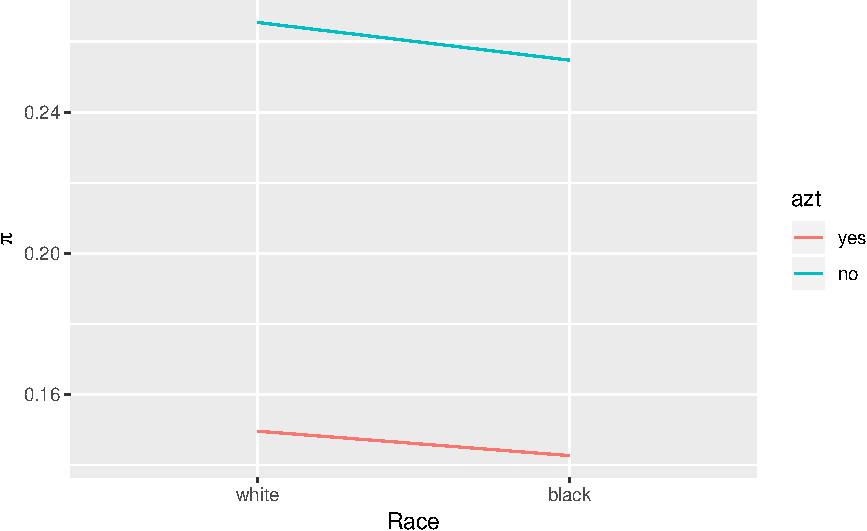
\includegraphics[width=0.7\linewidth]{_main_files/figure-latex/probaids-1} 

}

\caption{Conditional probability of developing AIDS symptoms\label{probaids}}\label{fig:probaids}
\end{figure}

Obviously, less probability is likely occur when the patient dose AZT directly. In Figure \ref{probaids}, the probability differs between AZT usage, while not between race. Now we can estimate the number of successes by

\[\{ \hat\mu_{ij} = n_{i+}\hat\pi_{j \mid i} \}\]

\begin{Shaded}
\begin{Highlighting}[]
\NormalTok{pred_prob }\OperatorTok\StringTok{ }
\StringTok{  }\KeywordTok{mutate}\NormalTok{(}\DataTypeTok{yes_fit =}\NormalTok{ (yes }\OperatorTok{+}\StringTok{ }\NormalTok{no) }\OperatorTok{*}\StringTok{ }\NormalTok{pred_prob,}
         \DataTypeTok{no_fit =}\NormalTok{ (yes }\OperatorTok{+}\StringTok{ }\NormalTok{no) }\OperatorTok{*}\StringTok{ }\NormalTok{(}\DecValTok{1} \OperatorTok{-}\StringTok{ }\NormalTok{pred_prob)) }\OperatorTok\StringTok{ }
\StringTok{  }\KeywordTok{arrange}\NormalTok{(}\KeywordTok{desc}\NormalTok{(race), }\KeywordTok{desc}\NormalTok{(azt)) }\OperatorTok\StringTok{ }
\StringTok{  }\KeywordTok{select}\NormalTok{(race, azt, yes, yes_fit, no, no_fit, pred_prob)}
\end{Highlighting}
\end{Shaded}

\begin{verbatim}
# A tibble: 4 x 7
  race  azt     yes yes_fit    no no_fit pred_prob
  <fct> <fct> <dbl>   <dbl> <dbl>  <dbl>     <dbl>
1 black no       12   14.0     43   41.0     0.255
2 black yes      11    8.99    52   54.0     0.143
3 white no       32   30.0     81   83.0     0.265
4 white yes      14   16.0     93   91.0     0.150
\end{verbatim}

It can be estimated as

\begin{Shaded}
\begin{Highlighting}[]
\NormalTok{pred_prob }\OperatorTok\StringTok{ }
\StringTok{  }\KeywordTok{mutate}\NormalTok{(}\DataTypeTok{yes_fit =}\NormalTok{ (yes }\OperatorTok{+}\StringTok{ }\NormalTok{no) }\OperatorTok{*}\StringTok{ }\NormalTok{pred_prob }\OperatorTok\StringTok{ }\KeywordTok{round}\NormalTok{(}\DataTypeTok{digits =} \DecValTok{1}\NormalTok{),}
         \DataTypeTok{no_fit =}\NormalTok{ (yes }\OperatorTok{+}\StringTok{ }\NormalTok{no) }\OperatorTok{*}\StringTok{ }\NormalTok{(}\DecValTok{1} \OperatorTok{-}\StringTok{ }\NormalTok{pred_prob) }\OperatorTok\StringTok{ }\KeywordTok{round}\NormalTok{(}\DataTypeTok{digits =} \DecValTok{1}\NormalTok{)) }\OperatorTok\StringTok{ }
\StringTok{  }\KeywordTok{unite}\NormalTok{(}\StringTok{"Yes"}\NormalTok{, }\KeywordTok{starts_with}\NormalTok{(}\StringTok{"yes"}\NormalTok{), }\DataTypeTok{sep =} \StringTok{" vs "}\NormalTok{) }\OperatorTok\StringTok{ }
\StringTok{  }\KeywordTok{unite}\NormalTok{(}\StringTok{"No"}\NormalTok{, }\KeywordTok{starts_with}\NormalTok{(}\StringTok{"no"}\NormalTok{), }\DataTypeTok{sep =} \StringTok{" vs "}\NormalTok{)}
\end{Highlighting}
\end{Shaded}

\begin{verbatim}
# A tibble: 4 x 5
  race  azt   Yes        No         pred_prob
  <fct> <fct> <chr>      <chr>          <dbl>
1 white yes   14 vs 10.7 93 vs 96.3     0.150
2 white no    32 vs 33.9 81 vs 79.1     0.265
3 black yes   11 vs 6.3  52 vs 56.7     0.143
4 black no    12 vs 16.5 43 vs 38.5     0.255
\end{verbatim}

In sum,

\begin{Shaded}
\begin{Highlighting}[]
\NormalTok{pred_prob }\OperatorTok\StringTok{ }
\StringTok{  }\KeywordTok{mutate}\NormalTok{(}\DataTypeTok{yes_fit =} \KeywordTok{round}\NormalTok{((yes }\OperatorTok{+}\StringTok{ }\NormalTok{no) }\OperatorTok{*}\StringTok{ }\NormalTok{pred_prob, }\DataTypeTok{digits =} \DecValTok{1}\NormalTok{),}
         \DataTypeTok{no_fit =} \KeywordTok{round}\NormalTok{((yes }\OperatorTok{+}\StringTok{ }\NormalTok{no) }\OperatorTok{*}\StringTok{ }\NormalTok{(}\DecValTok{1} \OperatorTok{-}\StringTok{ }\NormalTok{pred_prob), }\DataTypeTok{digits =} \DecValTok{1}\NormalTok{),}
         \DataTypeTok{pred_no =} \KeywordTok{round}\NormalTok{(}\DecValTok{1} \OperatorTok{-}\StringTok{ }\NormalTok{pred_prob, }\DataTypeTok{digits =} \DecValTok{3}\NormalTok{),}
         \DataTypeTok{pred_prob =} \KeywordTok{round}\NormalTok{(pred_prob, }\DataTypeTok{digits =} \DecValTok{3}\NormalTok{)) }\OperatorTok\StringTok{ }
\StringTok{  }\KeywordTok{select}\NormalTok{(race, azt, pred_prob, pred_no, yes_fit, no_fit) }\OperatorTok\StringTok{ }
\StringTok{  }\KeywordTok{gather}\NormalTok{(yes_fit, no_fit, }\DataTypeTok{key =}\NormalTok{ fit, }\DataTypeTok{value =}\NormalTok{ count) }\OperatorTok
\StringTok{  }\KeywordTok{gather}\NormalTok{(pred_prob, pred_no, }\DataTypeTok{key =}\NormalTok{ prob, }\DataTypeTok{value =}\NormalTok{ pred) }\OperatorTok
\StringTok{  }\KeywordTok{mutate_if}\NormalTok{(is.numeric, }\ControlFlowTok{function}\NormalTok{(x) \{}
    \KeywordTok{cell_spec}\NormalTok{(x, }\DataTypeTok{bold =} \OtherTok{TRUE}\NormalTok{,}
              \DataTypeTok{color =} \KeywordTok{spec_color}\NormalTok{(}\OperatorTok{-}\NormalTok{x, }\DataTypeTok{end =} \FloatTok{.9}\NormalTok{),}
              \DataTypeTok{font_size =} \KeywordTok{spec_font_size}\NormalTok{(x, }\DataTypeTok{begin =} \DecValTok{10}\NormalTok{))}
\NormalTok{  \}) }\OperatorTok\StringTok{ }
\StringTok{  }\KeywordTok{group_by}\NormalTok{(race) }\OperatorTok\StringTok{ }
\StringTok{  }\KeywordTok{mutate}\NormalTok{(}\DataTypeTok{azt =} \KeywordTok{cell_spec}\NormalTok{(}
\NormalTok{    azt, }\DataTypeTok{color =} \StringTok{"white"}\NormalTok{, }\DataTypeTok{bold =} \OtherTok{TRUE}\NormalTok{,}
    \DataTypeTok{background =} \KeywordTok{spec_color}\NormalTok{(}\DecValTok{1}\OperatorTok{:}\DecValTok{2}\NormalTok{, }\DataTypeTok{begin =} \FloatTok{.2}\NormalTok{, }\DataTypeTok{end =} \FloatTok{.7}\NormalTok{, }\DataTypeTok{option =} \StringTok{"plasma"}\NormalTok{, }\DataTypeTok{direction =} \DecValTok{1}\NormalTok{)}
\NormalTok{  )) }\OperatorTok\StringTok{ }
\StringTok{  }\KeywordTok{ungroup}\NormalTok{(race) }\OperatorTok\StringTok{ }
\StringTok{  }\KeywordTok{spread}\NormalTok{(prob, pred) }\OperatorTok\StringTok{ }
\StringTok{  }\KeywordTok{spread}\NormalTok{(fit, count) }\OperatorTok\StringTok{ }
\StringTok{  }\KeywordTok{select}\NormalTok{(race, azt, pred_prob, pred_no, yes_fit, no_fit) }\OperatorTok\StringTok{ }
\StringTok{  }\KeywordTok{kable}\NormalTok{(}\DataTypeTok{escape =} \OtherTok{FALSE}\NormalTok{, }\DataTypeTok{format =} \StringTok{"latex"}\NormalTok{, }\DataTypeTok{row.names =} \OtherTok{FALSE}\NormalTok{, }\DataTypeTok{booktabs =} \OtherTok{TRUE}\NormalTok{,}
        \DataTypeTok{col.names =} \KeywordTok{c}\NormalTok{(}\StringTok{"Race"}\NormalTok{, }\StringTok{"AZT Use"}\NormalTok{, }\StringTok{"Yes"}\NormalTok{, }\StringTok{"No"}\NormalTok{, }\StringTok{"Yes"}\NormalTok{, }\StringTok{"No"}\NormalTok{),}
        \DataTypeTok{caption =} \StringTok{"Estimated probability and Fitted number"}\NormalTok{,}
        \DataTypeTok{align =} \StringTok{"c"}\NormalTok{) }\OperatorTok\StringTok{ }
\StringTok{  }\KeywordTok{kable_styling}\NormalTok{(}\DataTypeTok{bootstrap_options =} \StringTok{"striped"}\NormalTok{, }\DataTypeTok{latex_options =} \StringTok{"HOLD_position"}\NormalTok{, }\DataTypeTok{full_width =} \OtherTok{FALSE}\NormalTok{) }\OperatorTok\StringTok{ }
\StringTok{  }\KeywordTok{add_header_above}\NormalTok{(}\DataTypeTok{header =} \KeywordTok{c}\NormalTok{(}\StringTok{" "}\NormalTok{, }\StringTok{" "}\NormalTok{, }\StringTok{"Fitted Probability"}\NormalTok{ =}\StringTok{ }\DecValTok{2}\NormalTok{, }\StringTok{"Fitted number"}\NormalTok{ =}\StringTok{ }\DecValTok{2}\NormalTok{))}
\end{Highlighting}
\end{Shaded}

\hypertarget{appendix}{%
\section*{Appendix}\label{appendix}}
\addcontentsline{toc}{section}{Appendix}

We can also use contingency table form for \texttt{glm()}

\begin{Shaded}
\begin{Highlighting}[]
\NormalTok{aids }\OperatorTok\StringTok{ }
\StringTok{  }\KeywordTok{mutate}\NormalTok{(}\DataTypeTok{Sum =}\NormalTok{ yes }\OperatorTok{+}\StringTok{ }\NormalTok{no) }\OperatorTok\StringTok{ }
\StringTok{  }\KeywordTok{glm}\NormalTok{(yes}\OperatorTok{/}\NormalTok{Sum }\OperatorTok{~}\StringTok{ }\NormalTok{azt }\OperatorTok{+}\StringTok{ }\NormalTok{race, }\DataTypeTok{data =}\NormalTok{ ., }\DataTypeTok{weights =}\NormalTok{ Sum, }\DataTypeTok{family =} \KeywordTok{binomial}\NormalTok{())}
\end{Highlighting}
\end{Shaded}

\begin{verbatim}

Call:  glm(formula = yes/Sum ~ azt + race, family = binomial(), data = ., 
    weights = Sum)

Coefficients:
(Intercept)       aztyes    racewhite  
    -1.0736      -0.7195       0.0555  

Degrees of Freedom: 3 Total (i.e. Null);  1 Residual
Null Deviance:      8.35 
Residual Deviance: 1.38     AIC: 24.9
\end{verbatim}

\hypertarget{multinomial-responses}{%
\chapter{Multinomial Responses}\label{multinomial-responses}}

\begin{Shaded}
\begin{Highlighting}[]
\CommentTok{# wrangling data -------------------------------------}
\KeywordTok{library}\NormalTok{(tidyverse)}
\CommentTok{# library(data.table)}
\CommentTok{# fitting the models ---------------------------------}
\KeywordTok{library}\NormalTok{(VGAM)}
\CommentTok{# coloring tables -code will be hidden----------------}
\KeywordTok{library}\NormalTok{(formattable)}
\CommentTok{# https://stackoverflow.com/questions/34983822/how-to-have-r-formattable-rendered-to-pdf-output-and-how-to-have-percents-in-the}
\NormalTok{export_formattable <-}\StringTok{ }\ControlFlowTok{function}\NormalTok{(f, file, }\DataTypeTok{background =} \StringTok{"white"}\NormalTok{, }\DataTypeTok{delay =} \FloatTok{0.2}\NormalTok{, ...)}
\NormalTok{\{}
\NormalTok{  w <-}\StringTok{ }\KeywordTok{as.htmlwidget}\NormalTok{(f, ...)}
\NormalTok{  path <-}\StringTok{ }\NormalTok{htmltools}\OperatorTok{::}\KeywordTok{html_print}\NormalTok{(w, }\DataTypeTok{background =}\NormalTok{ background, }\DataTypeTok{viewer =} \OtherTok{NULL}\NormalTok{)}
\NormalTok{  url <-}\StringTok{ }\KeywordTok{paste0}\NormalTok{(}\StringTok{"file:///"}\NormalTok{, }\KeywordTok{gsub}\NormalTok{(}\StringTok{"}\CharTok{\textbackslash{}\textbackslash{}\textbackslash{}\textbackslash{}}\StringTok{"}\NormalTok{, }\StringTok{"/"}\NormalTok{, }\KeywordTok{normalizePath}\NormalTok{(path)))}
\NormalTok{  webshot}\OperatorTok{::}\KeywordTok{webshot}\NormalTok{(url,}
          \DataTypeTok{file =}\NormalTok{ file,}
          \DataTypeTok{selector =} \StringTok{".formattable_widget"}\NormalTok{,}
          \DataTypeTok{delay =}\NormalTok{ delay)}
\NormalTok{\}}
\end{Highlighting}
\end{Shaded}

\hypertarget{nomial-response}{%
\section{Nomial Response}\label{nomial-response}}

\hypertarget{alligator-food-choice}{%
\section*{Alligator Food Choice}\label{alligator-food-choice}}
\addcontentsline{toc}{section}{Alligator Food Choice}

\begin{Shaded}
\begin{Highlighting}[]
\NormalTok{(ali <-}\StringTok{ }\KeywordTok{read_delim}\NormalTok{(}\StringTok{"data/Alligators.dat"}\NormalTok{, }\DataTypeTok{delim =} \StringTok{" "}\NormalTok{))}
\end{Highlighting}
\end{Shaded}

\begin{verbatim}
# A tibble: 80 x 5
    lake gender  size  food count
   <dbl>  <dbl> <dbl> <dbl> <dbl>
 1     1      1     1     1     7
 2     1      1     1     2     1
 3     1      1     1     3     0
 4     1      1     1     4     0
 5     1      1     1     5     5
 6     1      1     2     1     4
 7     1      1     2     2     0
 8     1      1     2     3     0
 9     1      1     2     4     1
10     1      1     2     5     2
# ... with 70 more rows
\end{verbatim}

\begin{quote}
primary food choice of alligators: Fish(1), Invertible(2), Reptile(3), Bird(4), Other(5)
\end{quote}

\begin{itemize}
\tightlist
\item
  \texttt{lake}

  \begin{itemize}
  \tightlist
  \item
    \texttt{Hancock}(1)
  \item
    \texttt{Oklahoma}(2)
  \item
    \texttt{Trafford}(3)
  \item
    \texttt{George}(4)
  \end{itemize}
\item
  \texttt{gender}

  \begin{itemize}
  \tightlist
  \item
    \texttt{Male}(1)
  \item
    \texttt{Female}(2)
  \end{itemize}
\item
  \texttt{size}

  \begin{itemize}
  \tightlist
  \item
    \texttt{\textless{}=\ 2.3\ meters\ long}(1)
  \item
    \texttt{\textgreater{}\ 2.3\ meters\ long}(2)
  \end{itemize}
\end{itemize}

\begin{Shaded}
\begin{Highlighting}[]
\NormalTok{ali <-}
\StringTok{  }\NormalTok{ali }\OperatorTok\StringTok{ }
\StringTok{  }\KeywordTok{mutate_at}\NormalTok{(}
    \DataTypeTok{.vars =} \KeywordTok{vars}\NormalTok{(}\OperatorTok{-}\NormalTok{count),}
    \DataTypeTok{.funs =} \KeywordTok{funs}\NormalTok{(factor)}
\NormalTok{  ) }\OperatorTok\StringTok{ }
\StringTok{  }\KeywordTok{mutate}\NormalTok{(}\DataTypeTok{food =} \KeywordTok{fct_recode}\NormalTok{(}
\NormalTok{    food,}
    \StringTok{"fish"}\NormalTok{ =}\StringTok{ "1"}\NormalTok{,}
    \StringTok{"inverebrate"}\NormalTok{ =}\StringTok{ "2"}\NormalTok{,}
    \StringTok{"reptile"}\NormalTok{ =}\StringTok{ "3"}\NormalTok{,}
    \StringTok{"bird"}\NormalTok{ =}\StringTok{ "4"}\NormalTok{,}
    \StringTok{"other"}\NormalTok{ =}\StringTok{ "5"}
\NormalTok{  ))}
\end{Highlighting}
\end{Shaded}

Contingency table:

\begin{Shaded}
\begin{Highlighting}[]
\NormalTok{(ali_contin <-}
\StringTok{  }\NormalTok{ali }\OperatorTok\StringTok{ }
\StringTok{  }\KeywordTok{group_by}\NormalTok{(lake, gender, size) }\OperatorTok\StringTok{ }
\StringTok{  }\KeywordTok{spread}\NormalTok{(food, count))}
\end{Highlighting}
\end{Shaded}

\begin{verbatim}
# A tibble: 16 x 8
# Groups:   lake, gender, size [16]
   lake  gender size   fish inverebrate reptile  bird other
   <fct> <fct>  <fct> <dbl>       <dbl>   <dbl> <dbl> <dbl>
 1 1     1      1         7           1       0     0     5
 2 1     1      2         4           0       0     1     2
 3 1     2      1        16           3       2     2     3
 4 1     2      2         3           0       1     2     3
 5 2     1      1         2           2       0     0     1
 6 2     1      2        13           7       6     0     0
 7 2     2      1         3           9       1     0     2
 8 2     2      2         0           1       0     1     0
 9 3     1      1         3           7       1     0     1
10 3     1      2         8           6       6     3     5
11 3     2      1         2           4       1     1     4
12 3     2      2         0           1       0     0     0
13 4     1      1        13          10       0     2     2
14 4     1      2         9           0       0     1     2
15 4     2      1         3           9       1     0     1
16 4     2      2         8           1       0     0     1
\end{verbatim}

\hypertarget{baseline-category-logistic-model}{%
\section{Baseline-category logistic model}\label{baseline-category-logistic-model}}

In \texttt{cbind()}, \texttt{vglm()} takes final component as baseline. Here, we take \texttt{fish} as baseline: food categories are reversed.

\begin{Shaded}
\begin{Highlighting}[]
\NormalTok{(ali_base <-}
\StringTok{  }\NormalTok{ali_contin }\OperatorTok\StringTok{ }
\StringTok{  }\KeywordTok{vglm}\NormalTok{(}\KeywordTok{cbind}\NormalTok{(other, bird, reptile, inverebrate, fish) }\OperatorTok{~}\StringTok{ }\NormalTok{lake }\OperatorTok{+}\StringTok{ }\NormalTok{size,}
       \DataTypeTok{data =}\NormalTok{ ., }\DataTypeTok{family =} \KeywordTok{multinomial}\NormalTok{(),}
       \DataTypeTok{contrasts =} \KeywordTok{list}\NormalTok{(}\DataTypeTok{lake =} \KeywordTok{contr.treatment}\NormalTok{(}\DataTypeTok{n =} \DecValTok{4}\NormalTok{, }\DataTypeTok{base =} \DecValTok{4}\NormalTok{),}
                        \DataTypeTok{size =} \KeywordTok{contr.treatment}\NormalTok{(}\DataTypeTok{n =} \DecValTok{2}\NormalTok{, }\DataTypeTok{base =} \DecValTok{2}\NormalTok{)))) }\OperatorTok\StringTok{ }
\StringTok{  }\KeywordTok{summary}\NormalTok{()}
\end{Highlighting}
\end{Shaded}

\begin{verbatim}

Call:
vglm(formula = cbind(other, bird, reptile, inverebrate, fish) ~ 
    lake + size, family = multinomial(), data = ., contrasts = list(lake = contr.treatment(n = 4, 
    base = 4), size = contr.treatment(n = 2, base = 2)))


Pearson residuals:
                      Min     1Q  Median    3Q  Max
log(mu[,1]/mu[,5]) -1.587 -0.319 -0.0159 1.033 1.41
log(mu[,2]/mu[,5]) -0.987 -0.508 -0.1144 0.237 3.99
log(mu[,3]/mu[,5]) -0.830 -0.585 -0.2309 0.223 2.24
log(mu[,4]/mu[,5]) -1.372 -0.438 -0.0248 0.244 1.99

Coefficients: 
              Estimate Std. Error z value Pr(>|z|)    
(Intercept):1 -1.90427    0.52583   -3.62  0.00029 ***
(Intercept):2 -2.09308    0.66223   -3.16  0.00157 ** 
(Intercept):3 -3.31453    1.05307      NA       NA    
(Intercept):4 -1.54902    0.42492   -3.65  0.00027 ***
lake1:1        0.82620    0.55754    1.48  0.13838    
lake1:2        0.69512    0.78126    0.89  0.37361    
lake1:3        1.24278    1.18542    1.05  0.29446    
lake1:4       -1.65836    0.61288   -2.71  0.00681 ** 
lake2:1        0.00565    0.77657    0.01  0.99419    
lake2:2       -0.65321    1.20192   -0.54  0.58681    
lake2:3        2.45887    1.11811    2.20  0.02787 *  
lake2:4        0.93722    0.47191    1.99  0.04703 *  
lake3:1        1.51637    0.62143    2.44  0.01468 *  
lake3:2        1.08777    0.84167    1.29  0.19622    
lake3:3        2.93525    1.11639    2.63  0.00856 ** 
lake3:4        1.12198    0.49051    2.29  0.02217 *  
size1:1        0.33155    0.44825    0.74  0.45951    
size1:2       -0.63066    0.64247   -0.98  0.32629    
size1:3       -0.35126    0.58003   -0.61  0.54479    
size1:4        1.45820    0.39594    3.68  0.00023 ***
---
Signif. codes:  0 '***' 0.001 '**' 0.01 '*' 0.05 '.' 0.1 ' ' 1

Number of linear predictors:  4 

Names of linear predictors: 
log(mu[,1]/mu[,5]), log(mu[,2]/mu[,5]), log(mu[,3]/mu[,5]), log(mu[,4]/mu[,5])

Residual deviance: 52.5 on 44 degrees of freedom

Log-likelihood: -74.4 on 44 degrees of freedom

Number of iterations: 5 

Warning: Hauck-Donner effect detected in the following estimate(s):
'(Intercept):3'

Reference group is level  5  of the response
\end{verbatim}

\hypertarget{goodness-of-fit-2}{%
\subsection{Goodness of fit}\label{goodness-of-fit-2}}

\[H_0: \boldsymbol\beta = 0\]

\begin{Shaded}
\begin{Highlighting}[]
\NormalTok{ali_basegood <-}
\StringTok{  }\NormalTok{ali_contin }\OperatorTok\StringTok{ }
\StringTok{  }\KeywordTok{ungroup}\NormalTok{() }\OperatorTok\StringTok{ }
\StringTok{  }\KeywordTok{do}\NormalTok{(}
    \DataTypeTok{null_fit =} \KeywordTok{vglm}\NormalTok{(}\KeywordTok{cbind}\NormalTok{(other, bird, reptile, inverebrate, fish) }\OperatorTok{~}\StringTok{ }\DecValTok{1}\NormalTok{, }
                    \DataTypeTok{data =}\NormalTok{ ., }\DataTypeTok{family =} \KeywordTok{multinomial}\NormalTok{()),}
    \DataTypeTok{gender_fit =} \KeywordTok{vglm}\NormalTok{(}\KeywordTok{cbind}\NormalTok{(other, bird, reptile, inverebrate, fish) }\OperatorTok{~}\StringTok{ }\NormalTok{gender, }
                    \DataTypeTok{data =}\NormalTok{ ., }\DataTypeTok{family =} \KeywordTok{multinomial}\NormalTok{(),}
                    \DataTypeTok{contrasts =} \KeywordTok{list}\NormalTok{(}\DataTypeTok{gender =} \KeywordTok{contr.treatment}\NormalTok{(}\DataTypeTok{n =} \DecValTok{2}\NormalTok{, }\DataTypeTok{base =} \DecValTok{2}\NormalTok{))),}
    \DataTypeTok{size_fit =} \KeywordTok{vglm}\NormalTok{(}\KeywordTok{cbind}\NormalTok{(other, bird, reptile, inverebrate, fish) }\OperatorTok{~}\StringTok{ }\NormalTok{size, }
                    \DataTypeTok{data =}\NormalTok{ ., }\DataTypeTok{family =} \KeywordTok{multinomial}\NormalTok{(),}
                    \DataTypeTok{contrasts =} \KeywordTok{list}\NormalTok{(}\DataTypeTok{size =} \KeywordTok{contr.treatment}\NormalTok{(}\DataTypeTok{n =} \DecValTok{2}\NormalTok{, }\DataTypeTok{base =} \DecValTok{2}\NormalTok{))),}
    \DataTypeTok{lake_fit =} \KeywordTok{vglm}\NormalTok{(}\KeywordTok{cbind}\NormalTok{(other, bird, reptile, inverebrate, fish) }\OperatorTok{~}\StringTok{ }\NormalTok{lake, }
                    \DataTypeTok{data =}\NormalTok{ ., }\DataTypeTok{family =} \KeywordTok{multinomial}\NormalTok{(),}
                    \DataTypeTok{contrasts =} \KeywordTok{list}\NormalTok{(}\DataTypeTok{lake =} \KeywordTok{contr.treatment}\NormalTok{(}\DataTypeTok{n =} \DecValTok{4}\NormalTok{, }\DataTypeTok{base =} \DecValTok{4}\NormalTok{))),}
    \DataTypeTok{add_fit =} \KeywordTok{vglm}\NormalTok{(}\KeywordTok{cbind}\NormalTok{(other, bird, reptile, inverebrate, fish) }\OperatorTok{~}\StringTok{ }\NormalTok{lake }\OperatorTok{+}\StringTok{ }\NormalTok{size, }
                    \DataTypeTok{data =}\NormalTok{ ., }\DataTypeTok{family =} \KeywordTok{multinomial}\NormalTok{(),}
                   \DataTypeTok{contrasts =} \KeywordTok{list}\NormalTok{(}\DataTypeTok{lake =} \KeywordTok{contr.treatment}\NormalTok{(}\DataTypeTok{n =} \DecValTok{4}\NormalTok{, }\DataTypeTok{base =} \DecValTok{4}\NormalTok{),}
                                    \DataTypeTok{size =} \KeywordTok{contr.treatment}\NormalTok{(}\DataTypeTok{n =} \DecValTok{2}\NormalTok{, }\DataTypeTok{base =} \DecValTok{2}\NormalTok{))),}
    \DataTypeTok{full_fit =} \KeywordTok{vglm}\NormalTok{(}\KeywordTok{cbind}\NormalTok{(other, bird, reptile, inverebrate, fish) }\OperatorTok{~}\StringTok{ }\NormalTok{gender }\OperatorTok{+}\StringTok{ }\NormalTok{lake }\OperatorTok{+}\StringTok{ }\NormalTok{size, }
                    \DataTypeTok{data =}\NormalTok{ ., }\DataTypeTok{family =} \KeywordTok{multinomial}\NormalTok{(),}
                    \DataTypeTok{contrasts =} \KeywordTok{list}\NormalTok{(}\DataTypeTok{lake =} \KeywordTok{contr.treatment}\NormalTok{(}\DataTypeTok{n =} \DecValTok{4}\NormalTok{, }\DataTypeTok{base =} \DecValTok{4}\NormalTok{),}
                                     \DataTypeTok{size =} \KeywordTok{contr.treatment}\NormalTok{(}\DataTypeTok{n =} \DecValTok{2}\NormalTok{, }\DataTypeTok{base =} \DecValTok{2}\NormalTok{),}
                                     \DataTypeTok{gender =} \KeywordTok{contr.treatment}\NormalTok{(}\DataTypeTok{n =} \DecValTok{2}\NormalTok{, }\DataTypeTok{base =} \DecValTok{2}\NormalTok{)))}
\NormalTok{  )}
\end{Highlighting}
\end{Shaded}

\begin{Shaded}
\begin{Highlighting}[]
\NormalTok{each_mod <-}\StringTok{ }\ControlFlowTok{function}\NormalTok{(x, }\DataTypeTok{test =} \StringTok{"LRT"}\NormalTok{, ...) \{}
\NormalTok{  mod_name <-}
\StringTok{    }\KeywordTok{as.character}\NormalTok{(x[[}\DecValTok{1}\NormalTok{]]}\OperatorTok{@}\NormalTok{call)[}\DecValTok{2}\NormalTok{] }\OperatorTok\StringTok{ }
\StringTok{    }\KeywordTok{str_extract}\NormalTok{(}\DataTypeTok{pattern =} \StringTok{"(?<=~).*"}\NormalTok{) }\OperatorTok\StringTok{ }
\StringTok{    }\KeywordTok{str_trim}\NormalTok{()}
  \CommentTok{# mod_aov <- broom::tidy(anova(x[[1]], type = 1, test = "LRT"))}
  \CommentTok{# mod_aov %>% }
  \CommentTok{#   add_column(model = rep(mod_name, nrow(mod_aov)), .before = 1)}
\NormalTok{  broom}\OperatorTok{::}\KeywordTok{tidy}\NormalTok{(}\KeywordTok{anova}\NormalTok{(x[[}\DecValTok{1}\NormalTok{]], }\DataTypeTok{type =} \DecValTok{1}\NormalTok{, }\DataTypeTok{test =}\NormalTok{ test, ...)) }\OperatorTok\StringTok{ }
\StringTok{    }\KeywordTok{slice}\NormalTok{(}\KeywordTok{n}\NormalTok{()) }\OperatorTok\StringTok{ }
\StringTok{    }\KeywordTok{add_column}\NormalTok{(}\DataTypeTok{model =}\NormalTok{ mod_name, }\DataTypeTok{.before =} \DecValTok{1}\NormalTok{)}
\NormalTok{\}}
\CommentTok{#-----------}
\NormalTok{(ali_good <-}
\StringTok{  }\NormalTok{ali_basegood }\OperatorTok\StringTok{ }
\StringTok{  }\KeywordTok{map}\NormalTok{(each_mod, }\DataTypeTok{test =} \StringTok{"LRT"}\NormalTok{) }\OperatorTok\StringTok{ }
\StringTok{  }\KeywordTok{bind_rows}\NormalTok{()) }\OperatorTok\StringTok{ }
\StringTok{  }\NormalTok{pander}\OperatorTok{::}\KeywordTok{pander}\NormalTok{()}
\end{Highlighting}
\end{Shaded}

\begin{longtable}[]{@{}ccccccc@{}}
\toprule
\begin{minipage}[b]{0.22\columnwidth}\centering
model\strut
\end{minipage} & \begin{minipage}[b]{0.08\columnwidth}\centering
term\strut
\end{minipage} & \begin{minipage}[b]{0.05\columnwidth}\centering
df\strut
\end{minipage} & \begin{minipage}[b]{0.10\columnwidth}\centering
Deviance\strut
\end{minipage} & \begin{minipage}[b]{0.11\columnwidth}\centering
Resid..Df\strut
\end{minipage} & \begin{minipage}[b]{0.12\columnwidth}\centering
Resid..Dev\strut
\end{minipage} & \begin{minipage}[b]{0.12\columnwidth}\centering
p.value\strut
\end{minipage}\tabularnewline
\midrule
\endhead
\begin{minipage}[t]{0.22\columnwidth}\centering
1\strut
\end{minipage} & \begin{minipage}[t]{0.08\columnwidth}\centering
NULL\strut
\end{minipage} & \begin{minipage}[t]{0.05\columnwidth}\centering
\strut
\end{minipage} & \begin{minipage}[t]{0.10\columnwidth}\centering
\strut
\end{minipage} & \begin{minipage}[t]{0.11\columnwidth}\centering
60\strut
\end{minipage} & \begin{minipage}[t]{0.12\columnwidth}\centering
116.8\strut
\end{minipage} & \begin{minipage}[t]{0.12\columnwidth}\centering
\strut
\end{minipage}\tabularnewline
\begin{minipage}[t]{0.22\columnwidth}\centering
gender\strut
\end{minipage} & \begin{minipage}[t]{0.08\columnwidth}\centering
gender\strut
\end{minipage} & \begin{minipage}[t]{0.05\columnwidth}\centering
4\strut
\end{minipage} & \begin{minipage}[t]{0.10\columnwidth}\centering
2.104\strut
\end{minipage} & \begin{minipage}[t]{0.11\columnwidth}\centering
56\strut
\end{minipage} & \begin{minipage}[t]{0.12\columnwidth}\centering
114.7\strut
\end{minipage} & \begin{minipage}[t]{0.12\columnwidth}\centering
0.7166\strut
\end{minipage}\tabularnewline
\begin{minipage}[t]{0.22\columnwidth}\centering
size\strut
\end{minipage} & \begin{minipage}[t]{0.08\columnwidth}\centering
size\strut
\end{minipage} & \begin{minipage}[t]{0.05\columnwidth}\centering
4\strut
\end{minipage} & \begin{minipage}[t]{0.10\columnwidth}\centering
15.15\strut
\end{minipage} & \begin{minipage}[t]{0.11\columnwidth}\centering
56\strut
\end{minipage} & \begin{minipage}[t]{0.12\columnwidth}\centering
101.6\strut
\end{minipage} & \begin{minipage}[t]{0.12\columnwidth}\centering
0.004401\strut
\end{minipage}\tabularnewline
\begin{minipage}[t]{0.22\columnwidth}\centering
lake\strut
\end{minipage} & \begin{minipage}[t]{0.08\columnwidth}\centering
lake\strut
\end{minipage} & \begin{minipage}[t]{0.05\columnwidth}\centering
12\strut
\end{minipage} & \begin{minipage}[t]{0.10\columnwidth}\centering
43.2\strut
\end{minipage} & \begin{minipage}[t]{0.11\columnwidth}\centering
48\strut
\end{minipage} & \begin{minipage}[t]{0.12\columnwidth}\centering
73.57\strut
\end{minipage} & \begin{minipage}[t]{0.12\columnwidth}\centering
2.092e-05\strut
\end{minipage}\tabularnewline
\begin{minipage}[t]{0.22\columnwidth}\centering
lake + size\strut
\end{minipage} & \begin{minipage}[t]{0.08\columnwidth}\centering
size\strut
\end{minipage} & \begin{minipage}[t]{0.05\columnwidth}\centering
4\strut
\end{minipage} & \begin{minipage}[t]{0.10\columnwidth}\centering
21.09\strut
\end{minipage} & \begin{minipage}[t]{0.11\columnwidth}\centering
44\strut
\end{minipage} & \begin{minipage}[t]{0.12\columnwidth}\centering
52.48\strut
\end{minipage} & \begin{minipage}[t]{0.12\columnwidth}\centering
0.0003043\strut
\end{minipage}\tabularnewline
\begin{minipage}[t]{0.22\columnwidth}\centering
gender + lake + size\strut
\end{minipage} & \begin{minipage}[t]{0.08\columnwidth}\centering
size\strut
\end{minipage} & \begin{minipage}[t]{0.05\columnwidth}\centering
4\strut
\end{minipage} & \begin{minipage}[t]{0.10\columnwidth}\centering
17.6\strut
\end{minipage} & \begin{minipage}[t]{0.11\columnwidth}\centering
40\strut
\end{minipage} & \begin{minipage}[t]{0.12\columnwidth}\centering
50.26\strut
\end{minipage} & \begin{minipage}[t]{0.12\columnwidth}\centering
0.001477\strut
\end{minipage}\tabularnewline
\bottomrule
\end{longtable}

Each differene between next row represents each

\[G^2\Big[\text{simple} \mid \text{complex} \Big]\]

For example,

\[G^2\Big[(L + S) \mid (G + L + S) \Big] = 52.478 - 50.264 =  2.215\]

\hypertarget{estimating-probabilities}{%
\section{Estimating probabilities}\label{estimating-probabilities}}

\[\pi_j(\mathbf{x}) = \frac{\exp(\alpha_j + \boldsymbol\beta_j^T \mathbf{x})}{1 + \sum\limits_{h = 1}^{J - 1}\exp(\alpha_h + \boldsymbol\beta_h^T\mathbf{x})}\]

\begin{Shaded}
\begin{Highlighting}[]
\NormalTok{(ali_pred <-}
\StringTok{  }\NormalTok{ali_contin }\OperatorTok\StringTok{ }
\StringTok{  }\KeywordTok{ungroup}\NormalTok{() }\OperatorTok\StringTok{ }
\StringTok{  }\KeywordTok{select}\NormalTok{(lake, size) }\OperatorTok\StringTok{ }
\StringTok{  }\KeywordTok{bind_cols}\NormalTok{(}\KeywordTok{predict}\NormalTok{(ali_base, }\DataTypeTok{newdata =}\NormalTok{ ., }\DataTypeTok{type =} \StringTok{"response"}\NormalTok{) }\OperatorTok\StringTok{ }\KeywordTok{tbl_df}\NormalTok{()))}
\end{Highlighting}
\end{Shaded}

\begin{verbatim}
# A tibble: 16 x 7
   lake  size   other    bird reptile inverebrate  fish
   <fct> <fct>  <dbl>   <dbl>   <dbl>       <dbl> <dbl>
 1 1     1     0.254  0.0704   0.0475      0.0931 0.535
 2 1     2     0.194  0.141    0.0718      0.0231 0.570
 3 1     1     0.254  0.0704   0.0475      0.0931 0.535
 4 1     2     0.194  0.141    0.0718      0.0231 0.570
 5 2     1     0.0539 0.00882  0.0772      0.602  0.258
 6 2     2     0.0687 0.0294   0.195       0.249  0.458
 7 2     1     0.0539 0.00882  0.0772      0.602  0.258
 8 2     2     0.0687 0.0294   0.195       0.249  0.458
 9 3     1     0.174  0.0359   0.0888      0.517  0.184
10 3     2     0.201  0.108    0.202       0.193  0.296
11 3     1     0.174  0.0359   0.0888      0.517  0.184
12 3     2     0.201  0.108    0.202       0.193  0.296
13 4     1     0.0938 0.0297   0.0116      0.413  0.452
14 4     2     0.0979 0.0811   0.0239      0.140  0.657
15 4     1     0.0938 0.0297   0.0116      0.413  0.452
16 4     2     0.0979 0.0811   0.0239      0.140  0.657
\end{verbatim}

\hypertarget{cumulative-logits}{%
\section{Cumulative Logits}\label{cumulative-logits}}

\hypertarget{happiness-and-traumatic-events}{%
\subsection*{Happiness and Traumatic Events}\label{happiness-and-traumatic-events}}
\addcontentsline{toc}{subsection}{Happiness and Traumatic Events}

\begin{Shaded}
\begin{Highlighting}[]
\NormalTok{gss <-}\StringTok{ }\KeywordTok{read_delim}\NormalTok{(}\StringTok{"data/happiness.dat"}\NormalTok{, }\DataTypeTok{delim =} \StringTok{" "}\NormalTok{)}
\end{Highlighting}
\end{Shaded}

\begin{center}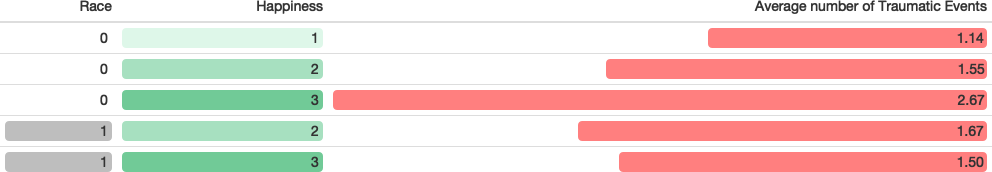
\includegraphics[width=0.7\linewidth]{_main_files/figure-latex/unnamed-chunk-105-1} \end{center}

\begin{itemize}
\tightlist
\item
  There are two explanatory variables in this dataset

  \begin{itemize}
  \tightlist
  \item
    total number of traumatic accidents: \(x_1\)
  \item
    whether they are Caucasian or African American: (\(x_2\), 1=black, 0=white)
  \end{itemize}
\item
  these variables are used to predict the degree of happiness, which is multinomial response measured on three point scale: 1=very happy, 2=pretty happy, 3=not too happy.
\end{itemize}

With this dataset, \emph{we want to figure out how to estimate response variable according to category and what explanatory factors influence on the response}. Look at the data. In case of white people, the more traumatic events they have had, the less happy they are. On the other hands, this relationships seems vague for black people.

Cumulative logit model is proper tool to analyze this data because response variable is ordinal response with categorical scales.

\hypertarget{cumulative-probability}{%
\subsection{Cumulative Probability}\label{cumulative-probability}}

Consider category ordering.

\begin{equation}
P(Y \le j \mid \mathbf{x}) = \pi_1(\mathbf{x}) + \cdots + \pi_j(\mathbf{x}), \quad j = 1,\ldots, J
\label{eq:prob}
\end{equation}

\hypertarget{cumulative-logits-1}{%
\subsection{Cumulative Logits}\label{cumulative-logits-1}}

Define logits for the cumulative probablities \(\eqref{eq:prob}\) as in the other settings.

\begin{center}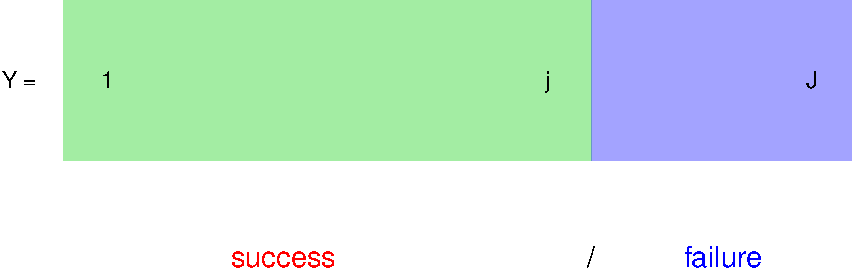
\includegraphics[width=0.7\linewidth]{_main_files/figure-latex/unnamed-chunk-106-1} \end{center}

\begin{equation}
\begin{split}
logit P(Y \le j \mid \mathbf{x}) & = \ln\frac{P(Y \le j \mid \mathbf{x})}{1 - P(Y \le j \mid \mathbf{x})} \\
& = \ln\frac{\pi_1(\mathbf{x}) + \cdots \pi_j (\mathbf{x})}{\pi_{j + 1}(\mathbf{x}) + \pi_J(\mathbf{x})}, \quad j = 1, \ldots J
\end{split}
\label{eq:logit}
\end{equation}

This is an ordinary logit for a binary response in which categories \(1\) to \(j\) from a single category \(j + 1\) to \(J\) from the second category.

\hypertarget{proportional-odds-property}{%
\subsection{Proportional Odds Property}\label{proportional-odds-property}}

Cumulative logit \(\eqref{eq:logit}\) can be modeled as GLM. Each \(logit P(Y \le j)\) becomes an ordinary logistic model for a binary response, i.e.~\(J - 1\) model with last one redundant category.

\begin{equation}
L_j(\mathbf{x}) := logit P(Y \le j \mid \mathbf{x}) = \alpha_j + \boldsymbol\beta^T\mathbf{x}, \quad j = 1, \ldots J - 1
\label{eq:model}
\end{equation}

\begin{figure}[H]

{\centering 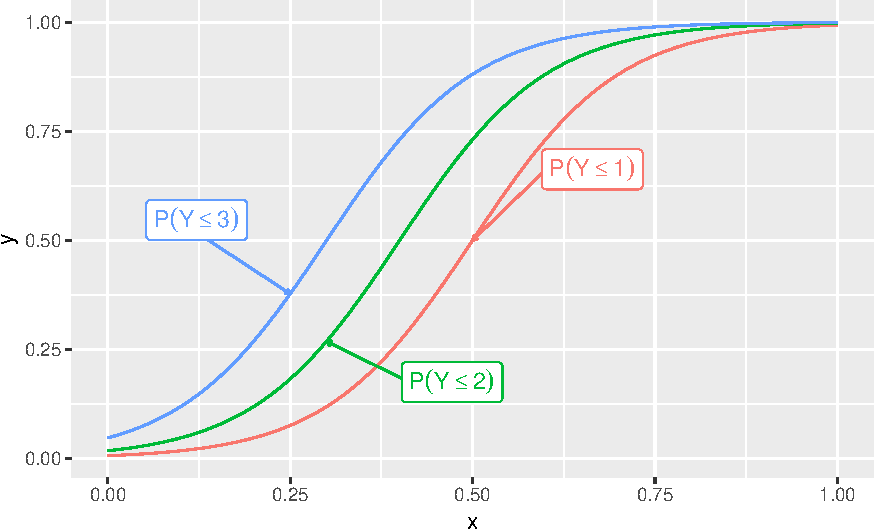
\includegraphics[width=0.7\linewidth]{_main_files/figure-latex/cumprob-1} 

}

\caption{Cumulative Logit for each three probabilities in a four-category case\label{cumprob}}\label{fig:cumprob}
\end{figure}

Althogh each logit has its own model, every logit shares the coefficient \(\boldsymbol\beta^T\), i.e.~\emph{parsimonious}. The only difference between each model is intercept terms. This setting is quite natural. See Figure \ref{cumprob}. Since the same effect is assumed for the models, the shapes of the fitted logit lines are same. It is moving horizontaly so that it would never catch up with the next line. If they were not of same shape by modeling \(\boldsymbol\beta_j^T\), the lines would cross each other. This contradicts to the construction of cumulative probability, \(P(Y \le j \mid \mathbf{x})\) increases in \(j\) for fixed \(\mathbf{x}\). This is why the model assumes \(\forall j : \boldsymbol\beta_j^T = \boldsymbol\beta^T\).

\begin{equation}
\begin{split}
L_j(\mathbf{x}_1) - L_j(\mathbf{x}_2) & = logit P(Y \le j \mid \mathbf{x}_1) - logit P(Y \le j \mid \mathbf{x}_2) \\
& = \ln\frac{P(Y \le j \mid \mathbf{x}_1) / P(Y > j \mid \mathbf{x}_1)}{P(Y \le j \mid \mathbf{x}_2) / P(Y > j \mid \mathbf{x}_2)} \\
& \overset{\eqref{eq:model}}{=} \boldsymbol\beta^T(\mathbf{x}_1 - \mathbf{x}_2)
\label{eq:propodds}
\end{split}
\end{equation}

The difference between log-odds of \(\le j\) at \(\mathbf{x}_1\) and of \(\mathbf{x}_2\) is \(\boldsymbol\beta^T(\mathbf{x}_1 - \mathbf{x}_2)\), i.e.~it is \emph{proportional to the distance between the two}. Since the proportionality constant applies to each logit, the model is called \emph{proportional odds model}. Also, an odds ratio of cumulative probailities is defined by \emph{cumulative odds ratio}.

\begin{equation}
\text{odds of making response}\: \le j \:\text{at}\: \mathbf{x} = \mathbf{x}_1 = \exp\big[\boldsymbol\beta^T(\mathbf{x}_1 - \mathbf{x}_2)\big]
\label{eq:oddr}
\end{equation}

Consider univariate case. \(\eqref{eq:oddr}\) implies the cumulative odds ratio equals \(e^\beta\) which is the \emph{constant cumulative odds ratio whenever} \(x_1 - x_2 = 1\).

\begin{figure}[H]

{\centering 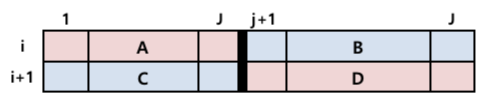
\includegraphics[width=0.7\linewidth]{images/unifodds} 

}

\caption{Uniform odds ratios AD/BC\label{unifodds}}\label{fig:unifodds}
\end{figure}

Figure \ref{unifodds} illustrates the uniform odds ratio \(\frac{AD}{BC} = \frac{A/B}{C/D}\) for all pair of adjustment rows and all response cut-point for the cumulative logit Uniform association model.

\hypertarget{relationship-between-y-and-x}{%
\subsection{Relationship between Y and x}\label{relationship-between-y-and-x}}

See Figure \ref{cumprob}. \(Y\) tends to be smaller at the higher values of \(x_i\). This can be less intuitive, so somtimes we reparameterize the model \(\eqref{eq:model}\) using \(-\boldsymbol\beta\) (\citet{McCullagh:1989aa}).

\begin{equation}
L_j(\mathbf{x}) = \alpha_j - \boldsymbol\beta^T\mathbf{x}, \quad j = 1, \ldots J - 1
\label{eq:reparam}
\end{equation}

In this model, \(Y\) tends to be large at higher values of \(\mathbf{x}_i\).

Or we can just \emph{recode higher level to be smaller value}, like in the data we are looking at.

\hypertarget{inference}{%
\subsection{Inference}\label{inference}}

\begin{Shaded}
\begin{Highlighting}[]
\NormalTok{(gss_contin <-}
\StringTok{  }\NormalTok{gss }\OperatorTok\StringTok{ }
\StringTok{  }\KeywordTok{mutate}\NormalTok{(}\DataTypeTok{happy =} \KeywordTok{fct_recode}\NormalTok{(happy, }\StringTok{"very"}\NormalTok{ =}\StringTok{ "1"}\NormalTok{, }\StringTok{"pretty"}\NormalTok{ =}\StringTok{ "2"}\NormalTok{, }\StringTok{"not"}\NormalTok{ =}\StringTok{ "3"}\NormalTok{)) }\OperatorTok\StringTok{ }
\StringTok{  }\KeywordTok{group_by}\NormalTok{(race, trauma, happy) }\OperatorTok\StringTok{ }
\StringTok{  }\KeywordTok{summarise}\NormalTok{(}\DataTypeTok{N =} \KeywordTok{n}\NormalTok{()) }\OperatorTok\StringTok{ }
\StringTok{  }\KeywordTok{spread}\NormalTok{(happy, N, }\DataTypeTok{fill =} \DecValTok{0}\NormalTok{))}
\end{Highlighting}
\end{Shaded}

\begin{verbatim}
# A tibble: 10 x 5
# Groups:   race, trauma [10]
   race  trauma  very pretty   not
   <fct>  <dbl> <dbl>  <dbl> <dbl>
 1 0          0     7     15     1
 2 0          1     8     12     1
 3 0          2     5     16     1
 4 0          3     1      9     1
 5 0          4     1      4     0
 6 0          5     0      0     2
 7 1          0     0      1     1
 8 1          1     0      3     1
 9 1          2     0      3     1
10 1          3     0      2     1
\end{verbatim}

\hypertarget{baseline-category-logit-model}{%
\subsection{Baseline-category logit model}\label{baseline-category-logit-model}}

We first try to fit model for nominal response, \emph{multinomial logistic regression}. Set baseline as \texttt{happy} = 3.

\[\ln\bigg(\frac{\pi_j}{\pi_3}\bigg) = \alpha_j + \boldsymbol\beta_j^T\mathbf{x}, \quad j = 1, 2\]

\begin{quote}
bcl-model
\end{quote}

\begin{Shaded}
\begin{Highlighting}[]
\NormalTok{(fit_baseline <-}
\StringTok{  }\NormalTok{gss_contin }\OperatorTok\StringTok{ }
\StringTok{  }\KeywordTok{vglm}\NormalTok{(}\KeywordTok{cbind}\NormalTok{(very, pretty, not) }\OperatorTok{~}\StringTok{ }\NormalTok{race }\OperatorTok{+}\StringTok{ }\NormalTok{trauma, }\DataTypeTok{data =}\NormalTok{ ., }\DataTypeTok{family =}\NormalTok{ multinomial)) }\OperatorTok\StringTok{  }\CommentTok{#<<}
\StringTok{  }\KeywordTok{summary}\NormalTok{()}
\end{Highlighting}
\end{Shaded}

\begin{verbatim}

Call:
vglm(formula = cbind(very, pretty, not) ~ race + trauma, family = multinomial, 
    data = .)


Pearson residuals:
                     Min     1Q   Median    3Q   Max
log(mu[,1]/mu[,3]) -1.06 -0.350 8.47e-06 0.206 0.820
log(mu[,2]/mu[,3]) -2.15 -0.473 1.87e-01 0.439 0.729

Coefficients: 
              Estimate Std. Error z value Pr(>|z|)    
(Intercept):1    2.556      0.820    3.12   0.0018 ** 
(Intercept):2    3.087      0.775    3.98  6.8e-05 ***
race1:1        -19.583   2662.468      NA       NA    
race1:2         -1.543      0.766   -2.01   0.0440 *  
trauma:1        -0.730      0.333   -2.19   0.0283 *  
trauma:2        -0.432      0.279   -1.55   0.1221    
---
Signif. codes:  0 '***' 0.001 '**' 0.01 '*' 0.05 '.' 0.1 ' ' 1

Number of linear predictors:  2 

Names of linear predictors: log(mu[,1]/mu[,3]), log(mu[,2]/mu[,3])

Residual deviance: 11.2 on 14 degrees of freedom

Log-likelihood: -19.6 on 14 degrees of freedom

Number of iterations: 17 

Warning: Hauck-Donner effect detected in the following estimate(s):
'race1:1'

Reference group is level  3  of the response
\end{verbatim}

Observe that this model nees to estimate \(6\) pameters. Consider the test

\[M_0: \text{without trauma variables} \Leftrightarrow \cdots = \beta_{j6} = 0 \qquad\text{vs}\qquad M_1: \text{this model}\]

\begin{quote}
bcl-goodness
\end{quote}

\begin{Shaded}
\begin{Highlighting}[]
\CommentTok{# lrtest(vglm(happy ~ race, data = gss, family = multinomial), fit_baseline)}
\NormalTok{(aov_dev <-}
\StringTok{  }\NormalTok{gss_contin }\OperatorTok\StringTok{ }
\StringTok{  }\KeywordTok{vglm}\NormalTok{(}\KeywordTok{cbind}\NormalTok{(very, pretty, not) }\OperatorTok{~}\StringTok{ }\NormalTok{race, }\DataTypeTok{data =}\NormalTok{ ., }\DataTypeTok{family =}\NormalTok{ multinomial) }\OperatorTok\StringTok{ }\CommentTok{# without trauma}
\StringTok{  }\KeywordTok{anova}\NormalTok{(fit_baseline, }\DataTypeTok{type =} \DecValTok{1}\NormalTok{, }\DataTypeTok{test =} \StringTok{"LRT"}\NormalTok{))}
\end{Highlighting}
\end{Shaded}

\begin{verbatim}
Analysis of Deviance Table

Model 1: cbind(very, pretty, not) ~ race
Model 2: cbind(very, pretty, not) ~ race + trauma
  Resid. Df Resid. Dev Df Deviance Pr(>Chi)  
1        16       16.4                       
2        14       11.2  2     5.21    0.074 .
---
Signif. codes:  0 '***' 0.001 '**' 0.01 '*' 0.05 '.' 0.1 ' ' 1
\end{verbatim}

\[G^2(M_0 \mid M_1) = \text{difference of deviance} = 5.205 \stackrel{M_0}{\approx} \chi^2(df = 2)\]

Since the p-value is 0.074, the model with \texttt{trauma} does not explain the data set well. This might be due to the missing \emph{ordinal information}.

\hypertarget{proportional-odds-model}{%
\subsection{Proportional odds model}\label{proportional-odds-model}}

Going back to the topic, we now fit \emph{cumulative logit model} \(\eqref{eq:model}\). It predicts the cumulative probability of a certain level of response on an ordinal scale. In other words, the purpose of analysis is to analyze how the ordinal response is predicted by explanatory variables.

\texttt{parallel\ =\ TRUE} of \texttt{family\ =\ cumulative()} link is implemented to assume proportional odds. To fit the other form of model \(\eqref{eq:reparam}\) of \citet{McCullagh:1989aa}, \texttt{family\ =\ propodds()} can also be considered.

\begin{quote}
prop-model
\end{quote}

\begin{Shaded}
\begin{Highlighting}[]
\NormalTok{(fit_cumul <-}
\StringTok{  }\NormalTok{gss_contin }\OperatorTok
\StringTok{  }\KeywordTok{vglm}\NormalTok{(}\KeywordTok{cbind}\NormalTok{(very, pretty, not) }\OperatorTok{~}\StringTok{ }\NormalTok{race }\OperatorTok{+}\StringTok{ }\NormalTok{trauma, }\DataTypeTok{data =}\NormalTok{ ., }\DataTypeTok{family =} \KeywordTok{cumulative}\NormalTok{(}\DataTypeTok{parallel =} \OtherTok{TRUE}\NormalTok{))) }\OperatorTok\StringTok{ }
\StringTok{  }\KeywordTok{summary}\NormalTok{()}
\end{Highlighting}
\end{Shaded}

\begin{verbatim}

Call:
vglm(formula = cbind(very, pretty, not) ~ race + trauma, family = cumulative(parallel = TRUE), 
    data = .)


Pearson residuals:
                  Min     1Q Median     3Q   Max
logit(P[Y<=1]) -0.658 -0.446 -0.309 0.0671 0.992
logit(P[Y<=2]) -2.799 -0.221  0.158 0.4730 0.874

Coefficients: 
              Estimate Std. Error z value Pr(>|z|)    
(Intercept):1   -0.518      0.338   -1.53   0.1255    
(Intercept):2    3.401      0.565    6.02  1.7e-09 ***
race1           -2.036      0.691   -2.95   0.0032 ** 
trauma          -0.406      0.181   -2.24   0.0249 *  
---
Signif. codes:  0 '***' 0.001 '**' 0.01 '*' 0.05 '.' 0.1 ' ' 1

Number of linear predictors:  2 

Names of linear predictors: logit(P[Y<=1]), logit(P[Y<=2])

Residual deviance: 12.7 on 16 degrees of freedom

Log-likelihood: -20.3 on 16 degrees of freedom

Number of iterations: 5 

No Hauck-Donner effect found in any of the estimates

Exponentiated coefficients:
 race1 trauma 
 0.131  0.667 
\end{verbatim}

\hypertarget{extra-power}{%
\subsection{Extra power}\label{extra-power}}

Compared to \protect\hyperlink{bcl-model}{bcl-model}, every effect in cummulative logit model is significant.

\begin{quote}
prop-goodness
\end{quote}

\begin{Shaded}
\begin{Highlighting}[]
\NormalTok{(aov_cumul <-}\StringTok{  }
\StringTok{  }\NormalTok{gss_contin }\OperatorTok\StringTok{ }
\StringTok{  }\KeywordTok{vglm}\NormalTok{(}\KeywordTok{cbind}\NormalTok{(very, pretty, not) }\OperatorTok{~}\StringTok{ }\NormalTok{race, }\DataTypeTok{data =}\NormalTok{ ., }\DataTypeTok{family =} \KeywordTok{cumulative}\NormalTok{(}\DataTypeTok{parallel =} \OtherTok{TRUE}\NormalTok{)) }\OperatorTok\StringTok{ }\CommentTok{# without trauma}
\StringTok{  }\KeywordTok{anova}\NormalTok{(fit_cumul, }\DataTypeTok{type =} \DecValTok{1}\NormalTok{, }\DataTypeTok{test =} \StringTok{"LRT"}\NormalTok{))}
\end{Highlighting}
\end{Shaded}

\begin{verbatim}
Analysis of Deviance Table

Model 1: cbind(very, pretty, not) ~ race
Model 2: cbind(very, pretty, not) ~ race + trauma
  Resid. Df Resid. Dev Df Deviance Pr(>Chi)  
1        17       17.8                       
2        16       12.7  1     5.07    0.024 *
---
Signif. codes:  0 '***' 0.001 '**' 0.01 '*' 0.05 '.' 0.1 ' ' 1
\end{verbatim}

Looking at the goodness-of-fit test versus non-\texttt{trauma} model.

\[G^2(M_0 \mid M_1) = 5.068 \stackrel{M_0}{\approx} \chi^2(df = 1)\]

We can see that the degrees of freedom is less than of baseline-category model. This gives the test more power.

\begin{figure}[H]

{\centering 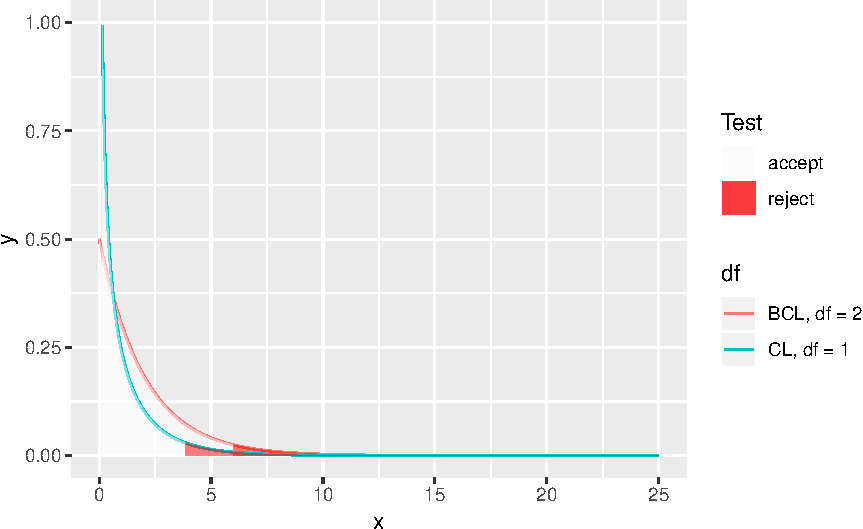
\includegraphics[width=0.7\linewidth]{_main_files/figure-latex/power-1} 

}

\caption{Benefits of utilizing the ordinality\label{power}}\label{fig:power}
\end{figure}

For same observed statistic, \(\chi^2\) distribution with small df can reject the test more easily thanks to its narrow tail. We can see with the eye in Figure \ref{power}.

\hypertarget{residual-degrees-of-freedom}{%
\subsection{Residual degrees of freedom}\label{residual-degrees-of-freedom}}

\begin{longtable}[]{@{}cc@{}}
\toprule
Saturated Model & Model\tabularnewline
\midrule
\endhead
\(n(J-1) = 20\) & \(n(J - 1)- p\)\tabularnewline
\bottomrule
\end{longtable}

\[
\text{residual df} = \begin{cases}
14 & \text{for baseline-category model} \\
16 & \text{for cumulative logit model}
\end{cases}
\]

\hypertarget{inference-concerning-cumulative-logits}{%
\subsection{Inference concerning cumulative logits}\label{inference-concerning-cumulative-logits}}

As other GLMs, cumulative logits can use \emph{Wald test statistic} or \emph{likelihood test statistic}.

\begin{Shaded}
\begin{Highlighting}[]
\KeywordTok{summary}\NormalTok{(fit_cumul, }\DataTypeTok{lrt0 =} \OtherTok{TRUE}\NormalTok{)}
\end{Highlighting}
\end{Shaded}

\begin{verbatim}

Call:
vglm(formula = cbind(very, pretty, not) ~ race + trauma, family = cumulative(parallel = TRUE), 
    data = .)


Pearson residuals:
                  Min     1Q Median     3Q   Max
logit(P[Y<=1]) -0.658 -0.446 -0.309 0.0671 0.992
logit(P[Y<=2]) -2.799 -0.221  0.158 0.4730 0.874

Likelihood ratio test coefficients: 
       Estimate z value Pr(>|z|)   
race1    -2.036   -3.04   0.0024 **
trauma   -0.406   -2.25   0.0244 * 
---
Signif. codes:  0 '***' 0.001 '**' 0.01 '*' 0.05 '.' 0.1 ' ' 1

Number of linear predictors:  2 

Names of linear predictors: logit(P[Y<=1]), logit(P[Y<=2])

Residual deviance: 12.7 on 16 degrees of freedom

Log-likelihood: -20.3 on 16 degrees of freedom

Number of iterations: 5 

Exponentiated coefficients:
 race1 trauma 
 0.131  0.667 
\end{verbatim}

We have already seen these in \protect\hyperlink{prop-model}{prop-model}, the model is estimated as

\[
\begin{cases}
logit P(Y \le 1 \mid \mathbf{x}) = -0.518 + \underset{p = 0.003}{-2.036} \text{race1} + \underset{p = 0.003}{-0.406} \text{trauma} \\
logit P(Y \le 2 \mid \mathbf{x}) = 3.401 + \underset{p = 0.003}{-2.036} \text{race1} + \underset{p = 0.003}{-0.406} \text{trauma}
\end{cases}
\]

The first equation is, when response variable is \texttt{very\ happy} and the Second logit model is the one when response variable is \texttt{pretty\ happy}. Coefficient estimates for explanatory variables(race and trauma) has less than 0.05 p-value, thus it is reasonable to use the parameters.

Denote that both effects are negative. \(\hat\beta_1 = -0.406\) suggest that the subject is not happy as she had have more and more traumatic events. \(\hat\beta_1 = -2.036\) indicates the blacks might be less happy compared to the whites. This \(race1\) variable shows lot difference. Given the number of traumatic events, the estimated odds for feeling very happy of observations in the white category is \(e^{race1} = 0.131\) times of observations in the black category. \citet{Agresti:2013aa} states that this estimates might be imprecise because these two categories are too imblanced.

\begin{verbatim}
# A tibble: 2 x 2
  race      N
  <fct> <int>
1 0        84
2 1        13
\end{verbatim}

This is reflected as wide confidence interval.

\begin{Shaded}
\begin{Highlighting}[]
\KeywordTok{confint}\NormalTok{(fit_cumul, }\DataTypeTok{method =} \StringTok{"profile"}\NormalTok{)}
\end{Highlighting}
\end{Shaded}

\begin{verbatim}
               2.5 % 97.5 %
(Intercept):1 -1.202  0.139
(Intercept):2  2.378  4.627
race1         -3.429 -0.716
trauma        -0.773 -0.052
\end{verbatim}

By construction, if we change the ordering reversely, the signs will be changed, either.

\hypertarget{checking-the-proportional-odds-assumption}{%
\subsection{Checking the proportional odds assumption}\label{checking-the-proportional-odds-assumption}}

Modeling each \(\boldsymbol\beta_j\) might fit better than single \(\boldsymbol\beta\). As mentioned, however, this results in non-parallelism of curves for different cumulative probabilites and makes them cross. Moreover, proportional odds model is simple to be summarized in terms of \emph{parsimony principle}. Conducting \emph{score test} or \emph{likelihood ratio test} for the nonparallel model helps us to choose between parallel or non-parallel models.

\begin{Shaded}
\begin{Highlighting}[]
\NormalTok{(beta_check <-}
\StringTok{  }\NormalTok{gss_contin }\OperatorTok\StringTok{ }
\StringTok{  }\KeywordTok{vglm}\NormalTok{(}\KeywordTok{cbind}\NormalTok{(very, pretty, not) }\OperatorTok{~}\StringTok{ }\NormalTok{., }\DataTypeTok{data =}\NormalTok{ ., }\DataTypeTok{family =} \KeywordTok{cumulative}\NormalTok{(}\DataTypeTok{parallel =} \OtherTok{FALSE}\NormalTok{)) }\OperatorTok
\StringTok{  }\KeywordTok{anova}\NormalTok{(fit_cumul, }\DataTypeTok{type =} \DecValTok{1}\NormalTok{, }\DataTypeTok{test =} \StringTok{"LRT"}\NormalTok{))}
\end{Highlighting}
\end{Shaded}

\begin{verbatim}
Analysis of Deviance Table

Model 1: cbind(very, pretty, not) ~ .
Model 2: cbind(very, pretty, not) ~ race + trauma
  Resid. Df Resid. Dev Df Deviance Pr(>Chi)
1        14       11.3                     
2        16       12.7 -2    -1.41     0.49
\end{verbatim}

p-value is 0.494. Thus, we can say that the proportional odds assumption is acceptable.

\hypertarget{nonparallelism}{%
\subsection{Nonparallelism}\label{nonparallelism}}

In some situation, this \emph{parallelism setting} might not fit. This proportional odds just follows proper order of cumulative probabilities. If we try to implement different odds, this order might be broken. In this case, \emph{some constraints} should be introduced.

\begin{itemize}
\tightlist
\item
  Adding additional terms

  \begin{itemize}
  \tightlist
  \item
    e.g.~interactions
  \end{itemize}
\item
  link function for which the response curve is nonsymmetric

  \begin{itemize}
  \tightlist
  \item
    e.g.~complementary log-log
  \end{itemize}
\item
  alternative ordinal model for which the more complex non-proportional-odds form
\item
  dispersion parameters
\item
  separate effects for each logit for some but not all predictors

  \begin{itemize}
  \tightlist
  \item
    e.g.~partial proportional odds
  \end{itemize}
\item
  baseline-category logit models and using the ordinality in an informal way in interpreting the associations
\end{itemize}

\hypertarget{interpretation}{%
\section{Interpretation}\label{interpretation}}

\hypertarget{comparing-cumulative-probabilities}{%
\subsection{Comparing cumulative probabilities}\label{comparing-cumulative-probabilities}}

Logistic regression model has been used odds ratio for interpretation. However, in case of ordinal variable, \emph{using cumulative probabilities can be more intuitive}\citep{Agresti:2018aa}. It is easier to conceptualize the size of effects. We can \emph{compare each probability}.

\begin{equation}
\begin{split}
& \hat{P}(Y = 1) = \hat{P}(Y \le 1) \\
& \hat{P}(Y = 2) = \hat{P}(Y \le 2) - \hat{P}(Y \le 1) \\
& \hat{P}(Y = 3) = \hat{P}(Y \le 3) - \hat{P}(Y \le 2) \\
& \vdots \\
& \hat{P}(Y = J) = 1 - \hat{P}(Y \le J - 1)
\label{eq:fitt}
\end{split}
\end{equation}

Using the fitted values of \(\eqref{eq:fitt}\), we can interpret the model in various aspects.

\begin{itemize}
\tightlist
\item
  At the extreme values, we can describe effects of quantitive one.
\item
  On the other hands, at the different categories, we can describe effects of qualitative one.
\end{itemize}

\begin{Shaded}
\begin{Highlighting}[]
\NormalTok{gss_pred <-}
\StringTok{  }\NormalTok{gss_contin }\OperatorTok\StringTok{ }
\StringTok{  }\KeywordTok{select}\NormalTok{(race, trauma) }\OperatorTok\StringTok{ }
\StringTok{  }\KeywordTok{bind_cols}\NormalTok{(}\KeywordTok{predict}\NormalTok{(fit_cumul, }\DataTypeTok{newdata =}\NormalTok{ ., }\DataTypeTok{type =} \StringTok{"response"}\NormalTok{) }\OperatorTok\StringTok{ }\KeywordTok{tbl_df}\NormalTok{())}
\end{Highlighting}
\end{Shaded}

\begin{center}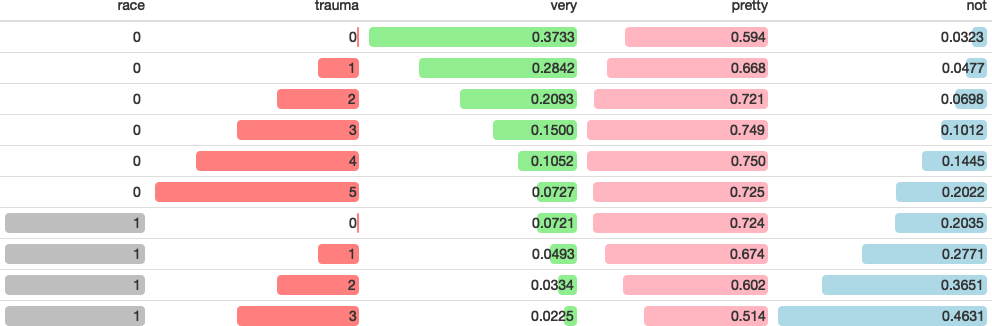
\includegraphics[width=0.7\linewidth]{_main_files/figure-latex/unnamed-chunk-116-1} \end{center}

For instance, when the white subject overcomes traumatic event zero, then \(\hat{P}(Y = 1 = \text{very happy}) = 0.373\) and \(\hat{P}(Y = 2 = \text{pretty happy}) = 0.594\).

\begin{figure}[H]

{\centering 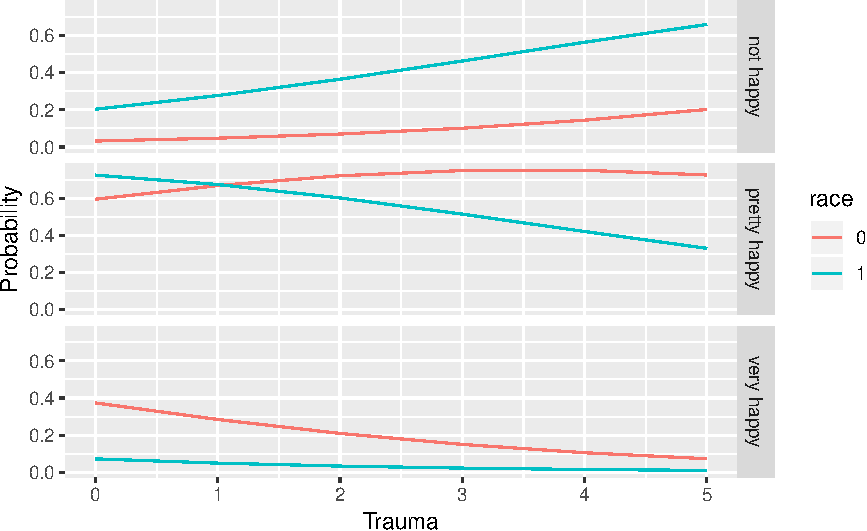
\includegraphics[width=0.7\linewidth]{_main_files/figure-latex/happyprob-1} 

}

\caption{Estimated value for each probability for happiness\label{happyprob}}\label{fig:happyprob}
\end{figure}

We can describe for each mean, minimum, and maximum numer of traumatic events.

\begin{verbatim}
# A tibble: 1 x 3
   mean   max   min
  <dbl> <dbl> <dbl>
1   2.1     5     0
\end{verbatim}

Look at the fitted probability of \emph{very happy} in Figure \ref{happyprob}.

\begin{itemize}
\tightlist
\item
  At the mean number, the difference between blacks and whites is almost \texttt{0.2}.
\item
  At the minimum, the difference is almost \texttt{0.4}.
\item
  At the maximum, on the other hand, the difference becomes very small.
\end{itemize}

Comparing blacks to whites, the change in whites is far more large. Again, black people are observed 13 times. Moreover, \emph{none of them has more than 3 traumatic events}.

\begin{verbatim}
# A tibble: 1 x 2
  race      N
  <fct> <int>
1 0         7
\end{verbatim}

\hypertarget{cheese-tasting}{%
\section{Cheese Tasting}\label{cheese-tasting}}

\hypertarget{data-description}{%
\subsection{Data Description}\label{data-description}}

This data is from \citet{McCullagh:1989aa}. Dr Graeme Newell obtained this data from experiments conducted to investigate the effect of taste on the various cheese additives. In this example, subjects were randomly assigned to taste one of four different cheeses. There are nine levels in response category.

\begin{itemize}
\tightlist
\item
  \(x\) = different cheeses: \texttt{A}, \texttt{B}, \texttt{C}, and \texttt{D}
\item
  \(y\) = \texttt{strong\ dislike}(1) to \texttt{excellent\ taste}(9)
\end{itemize}

Note that the respopnse variable is ordinal. To interpret the model \(\eqref{eq:model}\) easily, we would recode the taste factor reversely. \texttt{strong\ dislike} would be \texttt{9}, and \texttt{excellent\ taste} would be \texttt{1}.

\begin{Shaded}
\begin{Highlighting}[]
\NormalTok{newell <-}\StringTok{ }\KeywordTok{read_table}\NormalTok{(}\StringTok{"data/GLM175.txt"}\NormalTok{, }
                     \DataTypeTok{col_names =} \KeywordTok{str_c}\NormalTok{(}\StringTok{"taste"}\NormalTok{, }\DecValTok{9}\OperatorTok{:}\DecValTok{1}\NormalTok{, }\DataTypeTok{sep =} \StringTok{"_"}\NormalTok{))}
\NormalTok{newell <-}
\StringTok{  }\NormalTok{newell }\OperatorTok\StringTok{ }
\StringTok{  }\KeywordTok{add_column}\NormalTok{(}\DataTypeTok{cheese =}\NormalTok{ letters[}\DecValTok{1}\OperatorTok{:}\DecValTok{4}\NormalTok{], }\DataTypeTok{.before =} \DecValTok{1}\NormalTok{)}
\end{Highlighting}
\end{Shaded}

\begin{center}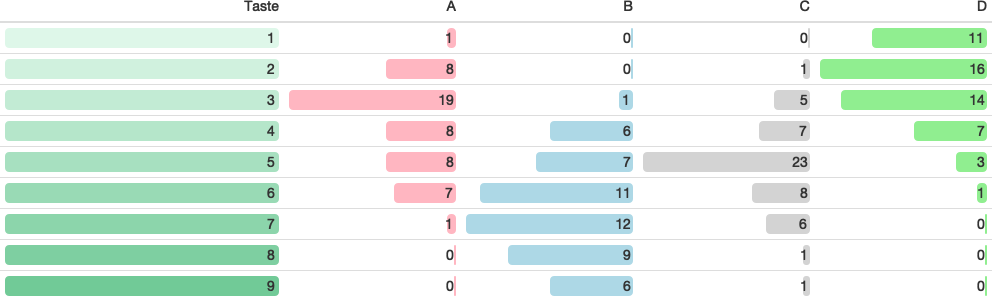
\includegraphics[width=0.7\linewidth]{_main_files/figure-latex/unnamed-chunk-121-1} \end{center}

In the above table, we can see the distribution of each count of taste vote, i.e.~the cheese variable has the ordering \emph{D \textgreater{} A \textgreater{} C \textgreater{} B}. However, this is an empirical measure and statistical modeling is needed to determine if there is really a difference between assessments of flavor depending on the type of cheese. Therefore, the researcher intended to identify that the result is reliable through a proportional-odds cumulative-logit model.

\hypertarget{proportional-odds-model-1}{%
\subsection{Proportional odds model}\label{proportional-odds-model-1}}

\begin{Shaded}
\begin{Highlighting}[]
\NormalTok{fit_vglm <-}\StringTok{ }\ControlFlowTok{function}\NormalTok{(.data, y_start, }\DataTypeTok{parallel =} \OtherTok{TRUE}\NormalTok{, ...) \{}
\NormalTok{  y_names <-}\StringTok{ }\KeywordTok{names}\NormalTok{(.data)}
\NormalTok{  y_mat <-}
\StringTok{    }\NormalTok{.data }\OperatorTok\StringTok{ }
\StringTok{    }\KeywordTok{select}\NormalTok{(}\KeywordTok{starts_with}\NormalTok{(y_start)) }\OperatorTok\StringTok{ }
\StringTok{    }\KeywordTok{as.matrix}\NormalTok{()}
\NormalTok{  .data }\OperatorTok\StringTok{ }
\StringTok{    }\KeywordTok{select}\NormalTok{(}\OperatorTok{-}\KeywordTok{starts_with}\NormalTok{(y_start)) }\OperatorTok\StringTok{ }
\StringTok{    }\KeywordTok{vglm}\NormalTok{(y_mat }\OperatorTok{~}\StringTok{ }\NormalTok{., }\DataTypeTok{data =}\NormalTok{ ., }\DataTypeTok{family =} \KeywordTok{cumulative}\NormalTok{(}\DataTypeTok{parallel =}\NormalTok{ parallel), ...)}
\NormalTok{\}}
\end{Highlighting}
\end{Shaded}

\begin{Shaded}
\begin{Highlighting}[]
\NormalTok{(fit_cheese <-}\StringTok{ }\KeywordTok{fit_vglm}\NormalTok{(newell, }\DataTypeTok{y_start =} \StringTok{"taste"}\NormalTok{, }\DataTypeTok{parallel =} \OtherTok{TRUE}\NormalTok{)) }\OperatorTok\StringTok{ }
\StringTok{  }\KeywordTok{summary}\NormalTok{(}\DataTypeTok{lrt0 =} \OtherTok{TRUE}\NormalTok{)}
\end{Highlighting}
\end{Shaded}

\begin{verbatim}

Call:
vglm(formula = y_mat ~ ., family = cumulative(parallel = parallel), 
    data = .)


Pearson residuals:
  logit(P[Y<=1]) logit(P[Y<=2]) logit(P[Y<=3]) logit(P[Y<=4])
1        -0.3071         -0.718         -0.843         2.1286
2         0.0615          0.612          0.184        -0.0796
3         0.0137         -0.805          0.174        -1.3671
4        -0.1256         -0.219         -0.632         0.1733
  logit(P[Y<=5]) logit(P[Y<=6]) logit(P[Y<=7]) logit(P[Y<=8])
1         0.2506         -1.191         -0.098          0.902
2        -2.1764          0.923          0.577          0.200
3         1.1730          0.328          0.453          0.571
4        -0.0755          0.996         -0.103         -0.585

Likelihood ratio test coefficients: 
        Estimate z value Pr(>|z|)    
cheeseb     3.35    8.44  < 2e-16 ***
cheesec     1.71    4.73  2.2e-06 ***
cheesed    -1.61   -4.37  1.2e-05 ***
---
Signif. codes:  0 '***' 0.001 '**' 0.01 '*' 0.05 '.' 0.1 ' ' 1

Number of linear predictors:  8 

Residual deviance: 20.3 on 21 degrees of freedom

Log-likelihood: -47.7 on 21 degrees of freedom

Number of iterations: 5 

Exponentiated coefficients:
cheeseb cheesec cheesed 
 28.555   5.528   0.199 
\end{verbatim}

Here, we have used \emph{dummy coding} with \(\beta_1 = 0\).

\begin{verbatim}
[1] a b c d
attr(,"contrasts")
  2 3 4
a 0 0 0
b 1 0 0
c 0 1 0
d 0 0 1
Levels: a b c d
\end{verbatim}

\begin{longtable}[]{@{}cccc@{}}
\caption{Table continues below}\tabularnewline
\toprule
\begin{minipage}[b]{0.18\columnwidth}\centering
coefficients\strut
\end{minipage} & \begin{minipage}[b]{0.21\columnwidth}\centering
logit(P{[}Y\textless{}=1{]})\strut
\end{minipage} & \begin{minipage}[b]{0.21\columnwidth}\centering
logit(P{[}Y\textless{}=2{]})\strut
\end{minipage} & \begin{minipage}[b]{0.21\columnwidth}\centering
logit(P{[}Y\textless{}=3{]})\strut
\end{minipage}\tabularnewline
\midrule
\endfirsthead
\toprule
\begin{minipage}[b]{0.18\columnwidth}\centering
coefficients\strut
\end{minipage} & \begin{minipage}[b]{0.21\columnwidth}\centering
logit(P{[}Y\textless{}=1{]})\strut
\end{minipage} & \begin{minipage}[b]{0.21\columnwidth}\centering
logit(P{[}Y\textless{}=2{]})\strut
\end{minipage} & \begin{minipage}[b]{0.21\columnwidth}\centering
logit(P{[}Y\textless{}=3{]})\strut
\end{minipage}\tabularnewline
\midrule
\endhead
\begin{minipage}[t]{0.18\columnwidth}\centering
(Intercept)\strut
\end{minipage} & \begin{minipage}[t]{0.21\columnwidth}\centering
-5.467\strut
\end{minipage} & \begin{minipage}[t]{0.21\columnwidth}\centering
-4.412\strut
\end{minipage} & \begin{minipage}[t]{0.21\columnwidth}\centering
-3.313\strut
\end{minipage}\tabularnewline
\begin{minipage}[t]{0.18\columnwidth}\centering
cheeseb\strut
\end{minipage} & \begin{minipage}[t]{0.21\columnwidth}\centering
3.352\strut
\end{minipage} & \begin{minipage}[t]{0.21\columnwidth}\centering
3.352\strut
\end{minipage} & \begin{minipage}[t]{0.21\columnwidth}\centering
3.352\strut
\end{minipage}\tabularnewline
\begin{minipage}[t]{0.18\columnwidth}\centering
cheesec\strut
\end{minipage} & \begin{minipage}[t]{0.21\columnwidth}\centering
1.71\strut
\end{minipage} & \begin{minipage}[t]{0.21\columnwidth}\centering
1.71\strut
\end{minipage} & \begin{minipage}[t]{0.21\columnwidth}\centering
1.71\strut
\end{minipage}\tabularnewline
\begin{minipage}[t]{0.18\columnwidth}\centering
cheesed\strut
\end{minipage} & \begin{minipage}[t]{0.21\columnwidth}\centering
-1.613\strut
\end{minipage} & \begin{minipage}[t]{0.21\columnwidth}\centering
-1.613\strut
\end{minipage} & \begin{minipage}[t]{0.21\columnwidth}\centering
-1.613\strut
\end{minipage}\tabularnewline
\bottomrule
\end{longtable}

\begin{longtable}[]{@{}cccc@{}}
\caption{Table continues below}\tabularnewline
\toprule
\begin{minipage}[b]{0.21\columnwidth}\centering
logit(P{[}Y\textless{}=4{]})\strut
\end{minipage} & \begin{minipage}[b]{0.21\columnwidth}\centering
logit(P{[}Y\textless{}=5{]})\strut
\end{minipage} & \begin{minipage}[b]{0.21\columnwidth}\centering
logit(P{[}Y\textless{}=6{]})\strut
\end{minipage} & \begin{minipage}[b]{0.21\columnwidth}\centering
logit(P{[}Y\textless{}=7{]})\strut
\end{minipage}\tabularnewline
\midrule
\endfirsthead
\toprule
\begin{minipage}[b]{0.21\columnwidth}\centering
logit(P{[}Y\textless{}=4{]})\strut
\end{minipage} & \begin{minipage}[b]{0.21\columnwidth}\centering
logit(P{[}Y\textless{}=5{]})\strut
\end{minipage} & \begin{minipage}[b]{0.21\columnwidth}\centering
logit(P{[}Y\textless{}=6{]})\strut
\end{minipage} & \begin{minipage}[b]{0.21\columnwidth}\centering
logit(P{[}Y\textless{}=7{]})\strut
\end{minipage}\tabularnewline
\midrule
\endhead
\begin{minipage}[t]{0.21\columnwidth}\centering
-2.244\strut
\end{minipage} & \begin{minipage}[t]{0.21\columnwidth}\centering
-0.9078\strut
\end{minipage} & \begin{minipage}[t]{0.21\columnwidth}\centering
0.04425\strut
\end{minipage} & \begin{minipage}[t]{0.21\columnwidth}\centering
1.546\strut
\end{minipage}\tabularnewline
\begin{minipage}[t]{0.21\columnwidth}\centering
3.352\strut
\end{minipage} & \begin{minipage}[t]{0.21\columnwidth}\centering
3.352\strut
\end{minipage} & \begin{minipage}[t]{0.21\columnwidth}\centering
3.352\strut
\end{minipage} & \begin{minipage}[t]{0.21\columnwidth}\centering
3.352\strut
\end{minipage}\tabularnewline
\begin{minipage}[t]{0.21\columnwidth}\centering
1.71\strut
\end{minipage} & \begin{minipage}[t]{0.21\columnwidth}\centering
1.71\strut
\end{minipage} & \begin{minipage}[t]{0.21\columnwidth}\centering
1.71\strut
\end{minipage} & \begin{minipage}[t]{0.21\columnwidth}\centering
1.71\strut
\end{minipage}\tabularnewline
\begin{minipage}[t]{0.21\columnwidth}\centering
-1.613\strut
\end{minipage} & \begin{minipage}[t]{0.21\columnwidth}\centering
-1.613\strut
\end{minipage} & \begin{minipage}[t]{0.21\columnwidth}\centering
-1.613\strut
\end{minipage} & \begin{minipage}[t]{0.21\columnwidth}\centering
-1.613\strut
\end{minipage}\tabularnewline
\bottomrule
\end{longtable}

\begin{longtable}[]{@{}cc@{}}
\toprule
\begin{minipage}[b]{0.22\columnwidth}\centering
logit(P{[}Y\textless{}=8{]})\strut
\end{minipage} & \begin{minipage}[b]{0.16\columnwidth}\centering
p\_value\strut
\end{minipage}\tabularnewline
\midrule
\endhead
\begin{minipage}[t]{0.22\columnwidth}\centering
3.106\strut
\end{minipage} & \begin{minipage}[t]{0.16\columnwidth}\centering
\strut
\end{minipage}\tabularnewline
\begin{minipage}[t]{0.22\columnwidth}\centering
3.352\strut
\end{minipage} & \begin{minipage}[t]{0.16\columnwidth}\centering
2.485e-15\strut
\end{minipage}\tabularnewline
\begin{minipage}[t]{0.22\columnwidth}\centering
1.71\strut
\end{minipage} & \begin{minipage}[t]{0.16\columnwidth}\centering
4.573e-06\strut
\end{minipage}\tabularnewline
\begin{minipage}[t]{0.22\columnwidth}\centering
-1.613\strut
\end{minipage} & \begin{minipage}[t]{0.16\columnwidth}\centering
1.962e-05\strut
\end{minipage}\tabularnewline
\bottomrule
\end{longtable}

Every \(\beta_j\) is significant. Recall that the dummy coding with \(\beta_1 = 0\) leads to

\[logitP(Y \le j \mid x = \text{cheese}\: l) = \beta_1 - \beta_l = -\beta_l\]

Then the effect estimates \(\hat\beta_1 = 3.352\) and \(\hat\beta_2 = 1.71\) suggest that the odds ratio of Cheese \texttt{B} and \texttt{C} is smaller than for Cheese \texttt{A}. For example, the estimated log odds ratio of Cheese C to A is \(-3.352\), and the tendency of C to receive a good response is \(\exp(-3.352) = 0.035\) times lower than that of A. Also, the possibility that the response of D is \(\exp(1.613) = 5.017\) times higher than the estimated odds of A. We see that the implied ordering of cheeses in terms of quality is \emph{D \textgreater{} A \textgreater{} C \textgreater{} B}.

\hypertarget{effect}{%
\subsection{Effect}\label{effect}}

\begin{Shaded}
\begin{Highlighting}[]
\CommentTok{# type 3 error, and type 1 here is equivalent to type 3}
\NormalTok{cheese_eff <-}\StringTok{ }\KeywordTok{anova}\NormalTok{(fit_cheese, }\DataTypeTok{type =} \DecValTok{1}\NormalTok{, }\DataTypeTok{test =} \StringTok{"LRT"}\NormalTok{)}
\end{Highlighting}
\end{Shaded}

\begin{longtable}[]{@{}cccccc@{}}
\caption{Analysis of Deviance Table (Type I tests: terms added sequentially from}\tabularnewline
\toprule
\begin{minipage}[b]{0.15\columnwidth}\centering
~\strut
\end{minipage} & \begin{minipage}[b]{0.06\columnwidth}\centering
Df\strut
\end{minipage} & \begin{minipage}[b]{0.13\columnwidth}\centering
Deviance\strut
\end{minipage} & \begin{minipage}[b]{0.14\columnwidth}\centering
Resid. Df\strut
\end{minipage} & \begin{minipage}[b]{0.15\columnwidth}\centering
Resid. Dev\strut
\end{minipage} & \begin{minipage}[b]{0.15\columnwidth}\centering
Pr(\textgreater{}Chi)\strut
\end{minipage}\tabularnewline
\midrule
\endfirsthead
\toprule
\begin{minipage}[b]{0.15\columnwidth}\centering
~\strut
\end{minipage} & \begin{minipage}[b]{0.06\columnwidth}\centering
Df\strut
\end{minipage} & \begin{minipage}[b]{0.13\columnwidth}\centering
Deviance\strut
\end{minipage} & \begin{minipage}[b]{0.14\columnwidth}\centering
Resid. Df\strut
\end{minipage} & \begin{minipage}[b]{0.15\columnwidth}\centering
Resid. Dev\strut
\end{minipage} & \begin{minipage}[b]{0.15\columnwidth}\centering
Pr(\textgreater{}Chi)\strut
\end{minipage}\tabularnewline
\midrule
\endhead
\begin{minipage}[t]{0.15\columnwidth}\centering
\textbf{NULL}\strut
\end{minipage} & \begin{minipage}[t]{0.06\columnwidth}\centering
\strut
\end{minipage} & \begin{minipage}[t]{0.13\columnwidth}\centering
\strut
\end{minipage} & \begin{minipage}[t]{0.14\columnwidth}\centering
24\strut
\end{minipage} & \begin{minipage}[t]{0.15\columnwidth}\centering
168.8\strut
\end{minipage} & \begin{minipage}[t]{0.15\columnwidth}\centering
\strut
\end{minipage}\tabularnewline
\begin{minipage}[t]{0.15\columnwidth}\centering
\textbf{cheese}\strut
\end{minipage} & \begin{minipage}[t]{0.06\columnwidth}\centering
3\strut
\end{minipage} & \begin{minipage}[t]{0.13\columnwidth}\centering
148.5\strut
\end{minipage} & \begin{minipage}[t]{0.14\columnwidth}\centering
21\strut
\end{minipage} & \begin{minipage}[t]{0.15\columnwidth}\centering
20.31\strut
\end{minipage} & \begin{minipage}[t]{0.15\columnwidth}\centering
5.679e-32\strut
\end{minipage}\tabularnewline
\bottomrule
\end{longtable}

We can see \texttt{cheese} is significant.

\hypertarget{proportional-odds-assumption}{%
\subsection{Proportional odds assumption}\label{proportional-odds-assumption}}

We try to test proportional odds assumption using LRT.

\begin{Shaded}
\begin{Highlighting}[]
\NormalTok{cheese_assume <-}
\StringTok{  }\NormalTok{fit_cheese }\OperatorTok\StringTok{ }
\StringTok{  }\KeywordTok{anova}\NormalTok{(}
    \KeywordTok{fit_vglm}\NormalTok{(newell, }\DataTypeTok{y_start =} \StringTok{"taste"}\NormalTok{, }\DataTypeTok{parallel =} \OtherTok{FALSE}\NormalTok{),}
    \DataTypeTok{type =} \DecValTok{1}\NormalTok{,}
    \DataTypeTok{test =} \StringTok{"LRT"}
\NormalTok{  )}
\end{Highlighting}
\end{Shaded}

\begin{longtable}[]{@{}ccccc@{}}
\caption{Analysis of Deviance Table}\tabularnewline
\toprule
\begin{minipage}[b]{0.14\columnwidth}\centering
Resid. Df\strut
\end{minipage} & \begin{minipage}[b]{0.16\columnwidth}\centering
Resid. Dev\strut
\end{minipage} & \begin{minipage}[b]{0.06\columnwidth}\centering
Df\strut
\end{minipage} & \begin{minipage}[b]{0.13\columnwidth}\centering
Deviance\strut
\end{minipage} & \begin{minipage}[b]{0.13\columnwidth}\centering
Pr(\textgreater{}Chi)\strut
\end{minipage}\tabularnewline
\midrule
\endfirsthead
\toprule
\begin{minipage}[b]{0.14\columnwidth}\centering
Resid. Df\strut
\end{minipage} & \begin{minipage}[b]{0.16\columnwidth}\centering
Resid. Dev\strut
\end{minipage} & \begin{minipage}[b]{0.06\columnwidth}\centering
Df\strut
\end{minipage} & \begin{minipage}[b]{0.13\columnwidth}\centering
Deviance\strut
\end{minipage} & \begin{minipage}[b]{0.13\columnwidth}\centering
Pr(\textgreater{}Chi)\strut
\end{minipage}\tabularnewline
\midrule
\endhead
\begin{minipage}[t]{0.14\columnwidth}\centering
21\strut
\end{minipage} & \begin{minipage}[t]{0.16\columnwidth}\centering
20.31\strut
\end{minipage} & \begin{minipage}[t]{0.06\columnwidth}\centering
\strut
\end{minipage} & \begin{minipage}[t]{0.13\columnwidth}\centering
\strut
\end{minipage} & \begin{minipage}[t]{0.13\columnwidth}\centering
\strut
\end{minipage}\tabularnewline
\begin{minipage}[t]{0.14\columnwidth}\centering
0\strut
\end{minipage} & \begin{minipage}[t]{0.16\columnwidth}\centering
1.062e-12\strut
\end{minipage} & \begin{minipage}[t]{0.06\columnwidth}\centering
21\strut
\end{minipage} & \begin{minipage}[t]{0.13\columnwidth}\centering
20.31\strut
\end{minipage} & \begin{minipage}[t]{0.13\columnwidth}\centering
0.5018\strut
\end{minipage}\tabularnewline
\bottomrule
\end{longtable}

With univariate model, \emph{non-parallism produces saturated model}. Here non-parallel model has \(p = (J-1)(\text{cheese category} - 1) = (8)(4) = 32\). Thus, its df becomes \(n(J - 1) - p = 0\).

Testing this model as \emph{alternative hypothesis}, the p-value is \(0.502\). It can be seen that \emph{the proportional odds assumption of the model is valid}. The model will have 8 intercepts (one for each of the logit equations) and 3 slopes, for a total of 11 free parameters.

\hypertarget{comparing-probabilities}{%
\subsection{Comparing probabilities}\label{comparing-probabilities}}

\begin{Shaded}
\begin{Highlighting}[]
\NormalTok{cheese_pred <-}
\StringTok{  }\NormalTok{newell }\OperatorTok\StringTok{ }
\StringTok{  }\KeywordTok{select}\NormalTok{(cheese) }\OperatorTok\StringTok{ }
\StringTok{  }\KeywordTok{bind_cols}\NormalTok{(}\KeywordTok{predict}\NormalTok{(fit_cheese, }\DataTypeTok{newdata =}\NormalTok{ ., }\DataTypeTok{type =} \StringTok{"response"}\NormalTok{) }\OperatorTok\StringTok{ }\KeywordTok{tbl_df}\NormalTok{())}
\end{Highlighting}
\end{Shaded}

\begin{center}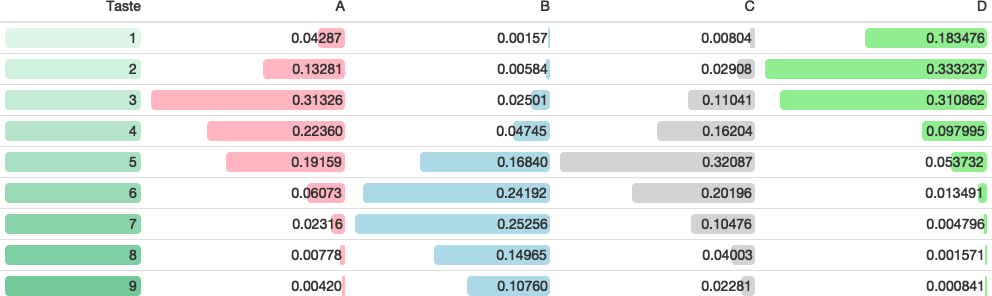
\includegraphics[width=0.7\linewidth]{_main_files/figure-latex/unnamed-chunk-133-1} \end{center}

For example, Subjects who had eaten \texttt{A} cheese answered that it taste \texttt{3}(quite tasty) about \(0.313\) of probability.

\begin{Shaded}
\begin{Highlighting}[]
\NormalTok{cheese_pred }\OperatorTok\StringTok{ }
\StringTok{  }\KeywordTok{gather}\NormalTok{(}\OperatorTok{-}\NormalTok{cheese, }\DataTypeTok{key =}\NormalTok{ tasty, }\DataTypeTok{value =}\NormalTok{ pp) }\OperatorTok\StringTok{ }
\StringTok{  }\KeywordTok{ggplot}\NormalTok{(}\KeywordTok{aes}\NormalTok{(}\DataTypeTok{x =}\NormalTok{ cheese, }\DataTypeTok{y =}\NormalTok{ pp)) }\OperatorTok{+}
\StringTok{  }\KeywordTok{geom_bar}\NormalTok{(}\KeywordTok{aes}\NormalTok{(}\DataTypeTok{fill =}\NormalTok{ tasty), }\DataTypeTok{stat =} \StringTok{"identity"}\NormalTok{) }\OperatorTok{+}
\StringTok{  }\KeywordTok{scale_fill_discrete}\NormalTok{(}\DataTypeTok{labels =} \DecValTok{1}\OperatorTok{:}\DecValTok{9}\NormalTok{) }\OperatorTok{+}
\StringTok{  }\KeywordTok{labs}\NormalTok{(}\DataTypeTok{x =} \StringTok{"Cheese"}\NormalTok{, }\DataTypeTok{y =} \StringTok{"Probability"}\NormalTok{)}
\end{Highlighting}
\end{Shaded}

\begin{figure}[H]

{\centering 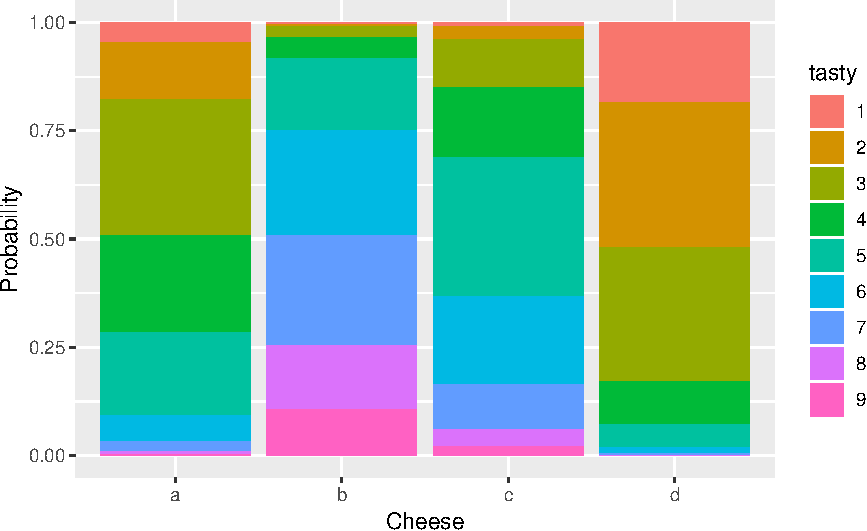
\includegraphics[width=0.7\linewidth]{_main_files/figure-latex/cheeseprob-1} 

}

\caption{Estimated Probability for each chease\label{cheeseprob}}\label{fig:cheeseprob}
\end{figure}

In Figure \ref{cheeseprob}, we can check how that cheese had been measured. The larger interval means larger probability. As the \texttt{tasty} is close to \texttt{1}, it means the cheese is preferable. \emph{D \textgreater{} A \textgreater{} C \textgreater{} B} of our first guess seems right.

\hypertarget{loglinear-models-for-contingency-tables}{%
\chapter{Loglinear Models for Contingency Tables}\label{loglinear-models-for-contingency-tables}}

\begin{Shaded}
\begin{Highlighting}[]
\KeywordTok{library}\NormalTok{(tidyverse)}
\end{Highlighting}
\end{Shaded}

\hypertarget{loglinear-models-for-two-way-tables}{%
\section{Loglinear models for Two-way tables}\label{loglinear-models-for-two-way-tables}}

\begin{quote}
Both variables are response variables.
\end{quote}

\hypertarget{association-between-responses}{%
\subsection{Association between responses}\label{association-between-responses}}

Consider \(I \times J\) contingency table \(\{ n_{ij} \}\). Then

\[n_{ij} \sim Poisson(\mu_{ij})\]

\hypertarget{loglinear-models-for-three-way-tables}{%
\section{Loglinear models for Three-way tables}\label{loglinear-models-for-three-way-tables}}

\hypertarget{alcohol-cigarette-and-marijuana-use}{%
\section*{Alcohol, cigarette, and marijuana use}\label{alcohol-cigarette-and-marijuana-use}}
\addcontentsline{toc}{section}{Alcohol, cigarette, and marijuana use}

\begin{Shaded}
\begin{Highlighting}[]
\NormalTok{(substance <-}
\StringTok{  }\KeywordTok{read_delim}\NormalTok{(}\StringTok{"data/Substance_use.dat"}\NormalTok{, }\DataTypeTok{delim =} \StringTok{" "}\NormalTok{) }\OperatorTok\StringTok{ }
\StringTok{  }\KeywordTok{mutate}\NormalTok{(}\DataTypeTok{alcohol =} \KeywordTok{str_trim}\NormalTok{(alcohol))) }\CommentTok{# due to messy data file}
\end{Highlighting}
\end{Shaded}

\begin{verbatim}
# A tibble: 8 x 4
  alcohol cigarettes marijuana count
  <chr>   <chr>      <chr>     <dbl>
1 yes     yes        yes         911
2 yes     yes        no          538
3 yes     no         yes          44
4 yes     no         no          456
5 no      yes        yes           3
6 no      yes        no           43
7 no      no         yes           2
8 no      no         no          279
\end{verbatim}

To fit loglinear model, long data format like this is easy.

\begin{Shaded}
\begin{Highlighting}[]
\NormalTok{substance <-}
\StringTok{  }\NormalTok{substance }\OperatorTok\StringTok{ }
\StringTok{  }\KeywordTok{mutate_if}\NormalTok{(is.character, factor) }\OperatorTok\StringTok{ }
\StringTok{  }\KeywordTok{mutate_if}\NormalTok{(is.factor, fct_rev)}
\end{Highlighting}
\end{Shaded}

Below is \emph{mutual independence model} \texttt{(A,\ C,\ M)}.

\begin{Shaded}
\begin{Highlighting}[]
\NormalTok{(subs_log <-}
\StringTok{  }\NormalTok{substance }\OperatorTok\StringTok{ }
\StringTok{  }\KeywordTok{glm}\NormalTok{(count }\OperatorTok{~}\StringTok{ }\NormalTok{alcohol }\OperatorTok{+}\StringTok{ }\NormalTok{cigarettes }\OperatorTok{+}\StringTok{ }\NormalTok{marijuana, }\DataTypeTok{data =}\NormalTok{ ., }\DataTypeTok{family =} \KeywordTok{poisson}\NormalTok{())) }\OperatorTok\StringTok{ }
\StringTok{  }\KeywordTok{summary}\NormalTok{()}
\end{Highlighting}
\end{Shaded}

\begin{verbatim}

Call:
glm(formula = count ~ alcohol + cigarettes + marijuana, family = poisson(), 
    data = .)

Deviance Residuals: 
     1       2       3       4       5       6       7       8  
 14.52   -7.82  -17.68    3.43  -12.44   -8.44   -8.83   19.64  

Coefficients:
             Estimate Std. Error z value Pr(>|z|)    
(Intercept)    6.2915     0.0367  171.56  < 2e-16 ***
alcoholno     -1.7851     0.0598  -29.87  < 2e-16 ***
cigarettesno  -0.6493     0.0442  -14.71  < 2e-16 ***
marijuanano    0.3154     0.0424    7.43  1.1e-13 ***
---
Signif. codes:  0 '***' 0.001 '**' 0.01 '*' 0.05 '.' 0.1 ' ' 1

(Dispersion parameter for poisson family taken to be 1)

    Null deviance: 2851.5  on 7  degrees of freedom
Residual deviance: 1286.0  on 4  degrees of freedom
AIC: 1343

Number of Fisher Scoring iterations: 6
\end{verbatim}

\hypertarget{chi-square-goodness-of-fit-tests}{%
\subsection{Chi-square Goodness-of-fit tests}\label{chi-square-goodness-of-fit-tests}}

\[G^2 = 2\sum n_{ijk}\ln\frac{n_{ijk}}{\hat\mu_{ijk}}\]

\[X^2 = \sum\frac{(n_{ijk} - \hat\mu_{ijk})^2}{\hat\mu_{ijk}}\]

with

\[\text{residual df} = \text{the number of cell counts} - \text{the number of non-redundant parameters}\]

\begin{Shaded}
\begin{Highlighting}[]
\NormalTok{subs_hierarchy <-}
\StringTok{  }\NormalTok{substance }\OperatorTok\StringTok{ }
\StringTok{  }\KeywordTok{do}\NormalTok{(}
    \DataTypeTok{indep =} \KeywordTok{glm}\NormalTok{(count }\OperatorTok{~}\StringTok{ }\NormalTok{alcohol }\OperatorTok{+}\StringTok{ }\NormalTok{cigarettes }\OperatorTok{+}\StringTok{ }\NormalTok{marijuana, }\DataTypeTok{data =}\NormalTok{ ., }\DataTypeTok{family =} \KeywordTok{poisson}\NormalTok{()),}
    \DataTypeTok{ac_m =} \KeywordTok{glm}\NormalTok{(count }\OperatorTok{~}\StringTok{ }\NormalTok{alcohol }\OperatorTok{+}\StringTok{ }\NormalTok{cigarettes }\OperatorTok{+}\StringTok{ }\NormalTok{marijuana }\OperatorTok{+}\StringTok{ }\NormalTok{alcohol}\OperatorTok{:}\NormalTok{cigarettes, }
               \DataTypeTok{data =}\NormalTok{ ., }\DataTypeTok{family =} \KeywordTok{poisson}\NormalTok{()),}
    \DataTypeTok{amcm =} \KeywordTok{glm}\NormalTok{(count }\OperatorTok{~}\StringTok{ }\NormalTok{alcohol }\OperatorTok{+}\StringTok{ }\NormalTok{cigarettes }\OperatorTok{+}\StringTok{ }\NormalTok{marijuana }\OperatorTok{+}\StringTok{ }\NormalTok{alcohol}\OperatorTok{:}\NormalTok{marijuana }\OperatorTok{+}\StringTok{ }\NormalTok{cigarettes}\OperatorTok{:}\NormalTok{marijuana, }
               \DataTypeTok{data =}\NormalTok{ ., }\DataTypeTok{family =} \KeywordTok{poisson}\NormalTok{()),}
    \DataTypeTok{acamcm =} \KeywordTok{glm}\NormalTok{(count }\OperatorTok{~}\StringTok{ }\NormalTok{alcohol }\OperatorTok{+}\StringTok{ }\NormalTok{cigarettes }\OperatorTok{+}\StringTok{ }\NormalTok{marijuana }\OperatorTok{+}\StringTok{ }\NormalTok{alcohol}\OperatorTok{:}\NormalTok{cigarettes }\OperatorTok{+}\StringTok{ }\NormalTok{alcohol}\OperatorTok{:}\NormalTok{marijuana }\OperatorTok{+}\StringTok{ }\NormalTok{cigarettes}\OperatorTok{:}\NormalTok{marijuana, }
               \DataTypeTok{data =}\NormalTok{ ., }\DataTypeTok{family =} \KeywordTok{poisson}\NormalTok{()),}
    \DataTypeTok{acm =} \KeywordTok{glm}\NormalTok{(count }\OperatorTok{~}\StringTok{ }\NormalTok{alcohol }\OperatorTok{*}\StringTok{ }\NormalTok{cigarettes }\OperatorTok{*}\StringTok{ }\NormalTok{marijuana, }
                 \DataTypeTok{data =}\NormalTok{ ., }\DataTypeTok{family =} \KeywordTok{poisson}\NormalTok{())}
\NormalTok{  )}
\end{Highlighting}
\end{Shaded}

\begin{Shaded}
\begin{Highlighting}[]
\NormalTok{good_loglin <-}\StringTok{ }\ControlFlowTok{function}\NormalTok{(x, }\DataTypeTok{test =} \StringTok{"LRT"}\NormalTok{, ...) \{}
\NormalTok{  mod_name <-}
\StringTok{    }\KeywordTok{as.character}\NormalTok{(x[[}\DecValTok{1}\NormalTok{]]}\OperatorTok{$}\NormalTok{call)[}\DecValTok{2}\NormalTok{] }\OperatorTok\StringTok{ }
\StringTok{    }\KeywordTok{str_extract}\NormalTok{(}\DataTypeTok{pattern =} \StringTok{"(?<=~).*"}\NormalTok{) }\OperatorTok\StringTok{ }
\StringTok{    }\KeywordTok{str_trim}\NormalTok{()}
\NormalTok{  broom}\OperatorTok{::}\KeywordTok{tidy}\NormalTok{(}\KeywordTok{anova}\NormalTok{(x[[}\DecValTok{1}\NormalTok{]], }\DataTypeTok{test =}\NormalTok{ test, ...)) }\OperatorTok\StringTok{ }
\StringTok{    }\KeywordTok{slice}\NormalTok{(}\KeywordTok{n}\NormalTok{()) }\OperatorTok\StringTok{ }
\StringTok{    }\KeywordTok{add_column}\NormalTok{(}\DataTypeTok{model =}\NormalTok{ mod_name, }\DataTypeTok{.before =} \DecValTok{1}\NormalTok{) }\OperatorTok\StringTok{ }
\StringTok{    }\KeywordTok{select}\NormalTok{(}\OperatorTok{-}\NormalTok{term)}
\NormalTok{\}}
\CommentTok{#-----------------------------------------------}
\NormalTok{(subs_good <-}
\StringTok{  }\NormalTok{subs_hierarchy }\OperatorTok\StringTok{ }
\StringTok{  }\KeywordTok{map}\NormalTok{(good_loglin, }\DataTypeTok{test =} \StringTok{"LRT"}\NormalTok{) }\OperatorTok\StringTok{ }
\StringTok{  }\KeywordTok{bind_rows}\NormalTok{()) }\OperatorTok\StringTok{ }
\StringTok{  }\NormalTok{pander}\OperatorTok{::}\KeywordTok{pander}\NormalTok{()}
\end{Highlighting}
\end{Shaded}

\begin{longtable}[]{@{}ccccc@{}}
\caption{Table continues below}\tabularnewline
\toprule
\begin{minipage}[b]{0.38\columnwidth}\centering
model\strut
\end{minipage} & \begin{minipage}[b]{0.06\columnwidth}\centering
df\strut
\end{minipage} & \begin{minipage}[b]{0.13\columnwidth}\centering
Deviance\strut
\end{minipage} & \begin{minipage}[b]{0.14\columnwidth}\centering
Resid..Df\strut
\end{minipage} & \begin{minipage}[b]{0.15\columnwidth}\centering
Resid..Dev\strut
\end{minipage}\tabularnewline
\midrule
\endfirsthead
\toprule
\begin{minipage}[b]{0.38\columnwidth}\centering
model\strut
\end{minipage} & \begin{minipage}[b]{0.06\columnwidth}\centering
df\strut
\end{minipage} & \begin{minipage}[b]{0.13\columnwidth}\centering
Deviance\strut
\end{minipage} & \begin{minipage}[b]{0.14\columnwidth}\centering
Resid..Df\strut
\end{minipage} & \begin{minipage}[b]{0.15\columnwidth}\centering
Resid..Dev\strut
\end{minipage}\tabularnewline
\midrule
\endhead
\begin{minipage}[t]{0.38\columnwidth}\centering
alcohol + cigarettes +
marijuana\strut
\end{minipage} & \begin{minipage}[t]{0.06\columnwidth}\centering
1\strut
\end{minipage} & \begin{minipage}[t]{0.13\columnwidth}\centering
55.91\strut
\end{minipage} & \begin{minipage}[t]{0.14\columnwidth}\centering
4\strut
\end{minipage} & \begin{minipage}[t]{0.15\columnwidth}\centering
1286\strut
\end{minipage}\tabularnewline
\begin{minipage}[t]{0.38\columnwidth}\centering
alcohol + cigarettes +
marijuana + alcohol:cigarettes\strut
\end{minipage} & \begin{minipage}[t]{0.06\columnwidth}\centering
1\strut
\end{minipage} & \begin{minipage}[t]{0.13\columnwidth}\centering
442.2\strut
\end{minipage} & \begin{minipage}[t]{0.14\columnwidth}\centering
3\strut
\end{minipage} & \begin{minipage}[t]{0.15\columnwidth}\centering
843.8\strut
\end{minipage}\tabularnewline
\begin{minipage}[t]{0.38\columnwidth}\centering
alcohol + cigarettes +
marijuana + alcohol:marijuana
+ cigarettes:marijuana\strut
\end{minipage} & \begin{minipage}[t]{0.06\columnwidth}\centering
1\strut
\end{minipage} & \begin{minipage}[t]{0.13\columnwidth}\centering
751.8\strut
\end{minipage} & \begin{minipage}[t]{0.14\columnwidth}\centering
2\strut
\end{minipage} & \begin{minipage}[t]{0.15\columnwidth}\centering
187.8\strut
\end{minipage}\tabularnewline
\begin{minipage}[t]{0.38\columnwidth}\centering
alcohol + cigarettes +
marijuana + alcohol:cigarettes
+ alcohol:marijuana +
cigarettes:marijuana\strut
\end{minipage} & \begin{minipage}[t]{0.06\columnwidth}\centering
1\strut
\end{minipage} & \begin{minipage}[t]{0.13\columnwidth}\centering
497\strut
\end{minipage} & \begin{minipage}[t]{0.14\columnwidth}\centering
1\strut
\end{minipage} & \begin{minipage}[t]{0.15\columnwidth}\centering
0.374\strut
\end{minipage}\tabularnewline
\begin{minipage}[t]{0.38\columnwidth}\centering
alcohol * cigarettes *
marijuana\strut
\end{minipage} & \begin{minipage}[t]{0.06\columnwidth}\centering
1\strut
\end{minipage} & \begin{minipage}[t]{0.13\columnwidth}\centering
0.374\strut
\end{minipage} & \begin{minipage}[t]{0.14\columnwidth}\centering
0\strut
\end{minipage} & \begin{minipage}[t]{0.15\columnwidth}\centering
-4.152e-14\strut
\end{minipage}\tabularnewline
\bottomrule
\end{longtable}

\begin{longtable}[]{@{}c@{}}
\toprule
\begin{minipage}[b]{0.18\columnwidth}\centering
p.value\strut
\end{minipage}\tabularnewline
\midrule
\endhead
\begin{minipage}[t]{0.18\columnwidth}\centering
7.575e-14\strut
\end{minipage}\tabularnewline
\begin{minipage}[t]{0.18\columnwidth}\centering
3.607e-98\strut
\end{minipage}\tabularnewline
\begin{minipage}[t]{0.18\columnwidth}\centering
1.623e-165\strut
\end{minipage}\tabularnewline
\begin{minipage}[t]{0.18\columnwidth}\centering
4.283e-110\strut
\end{minipage}\tabularnewline
\begin{minipage}[t]{0.18\columnwidth}\centering
0.5408\strut
\end{minipage}\tabularnewline
\bottomrule
\end{longtable}

From above \(G^2\), we compare reduced model to complex model

\[G^2(M_0 \mid M_1) = G^2(M_0) - G^2(M_1) \approx \chi^2\Big(df = df(M_0) - df(M_1)\Big)\]

\begin{Shaded}
\begin{Highlighting}[]
\NormalTok{subs_good }\OperatorTok\StringTok{ }
\StringTok{  }\KeywordTok{select}\NormalTok{(}\OperatorTok{-}\NormalTok{Deviance, }\OperatorTok{-}\NormalTok{p.value) }\OperatorTok\StringTok{ }
\StringTok{  }\KeywordTok{rename}\NormalTok{(}\DataTypeTok{alternative =}\NormalTok{ model) }\OperatorTok\StringTok{ }
\StringTok{  }\KeywordTok{mutate}\NormalTok{(}\DataTypeTok{goodness =} \KeywordTok{c}\NormalTok{(Resid..Dev[}\DecValTok{1}\NormalTok{], }\OperatorTok{-}\KeywordTok{diff}\NormalTok{(Resid..Dev)),}
         \DataTypeTok{df_good =} \KeywordTok{c}\NormalTok{(Resid..Df[}\DecValTok{1}\NormalTok{], }\OperatorTok{-}\KeywordTok{diff}\NormalTok{(Resid..Df))) }\OperatorTok\StringTok{ }
\StringTok{  }\KeywordTok{mutate}\NormalTok{(}\DataTypeTok{p_value =} \KeywordTok{pchisq}\NormalTok{(goodness, }\DataTypeTok{df =}\NormalTok{ df_good, }\DataTypeTok{lower.tail =} \OtherTok{FALSE}\NormalTok{)) }\OperatorTok\StringTok{ }
\StringTok{  }\NormalTok{pander}\OperatorTok{::}\KeywordTok{pander}\NormalTok{()}
\end{Highlighting}
\end{Shaded}

\begin{longtable}[]{@{}ccccc@{}}
\caption{Table continues below}\tabularnewline
\toprule
\begin{minipage}[b]{0.37\columnwidth}\centering
alternative\strut
\end{minipage} & \begin{minipage}[b]{0.06\columnwidth}\centering
df\strut
\end{minipage} & \begin{minipage}[b]{0.14\columnwidth}\centering
Resid..Df\strut
\end{minipage} & \begin{minipage}[b]{0.15\columnwidth}\centering
Resid..Dev\strut
\end{minipage} & \begin{minipage}[b]{0.15\columnwidth}\centering
goodness\strut
\end{minipage}\tabularnewline
\midrule
\endfirsthead
\toprule
\begin{minipage}[b]{0.37\columnwidth}\centering
alternative\strut
\end{minipage} & \begin{minipage}[b]{0.06\columnwidth}\centering
df\strut
\end{minipage} & \begin{minipage}[b]{0.14\columnwidth}\centering
Resid..Df\strut
\end{minipage} & \begin{minipage}[b]{0.15\columnwidth}\centering
Resid..Dev\strut
\end{minipage} & \begin{minipage}[b]{0.15\columnwidth}\centering
goodness\strut
\end{minipage}\tabularnewline
\midrule
\endhead
\begin{minipage}[t]{0.37\columnwidth}\centering
alcohol + cigarettes +
marijuana\strut
\end{minipage} & \begin{minipage}[t]{0.06\columnwidth}\centering
1\strut
\end{minipage} & \begin{minipage}[t]{0.14\columnwidth}\centering
4\strut
\end{minipage} & \begin{minipage}[t]{0.15\columnwidth}\centering
1286\strut
\end{minipage} & \begin{minipage}[t]{0.15\columnwidth}\centering
1286\strut
\end{minipage}\tabularnewline
\begin{minipage}[t]{0.37\columnwidth}\centering
alcohol + cigarettes +
marijuana + alcohol:cigarettes\strut
\end{minipage} & \begin{minipage}[t]{0.06\columnwidth}\centering
1\strut
\end{minipage} & \begin{minipage}[t]{0.14\columnwidth}\centering
3\strut
\end{minipage} & \begin{minipage}[t]{0.15\columnwidth}\centering
843.8\strut
\end{minipage} & \begin{minipage}[t]{0.15\columnwidth}\centering
442.2\strut
\end{minipage}\tabularnewline
\begin{minipage}[t]{0.37\columnwidth}\centering
alcohol + cigarettes +
marijuana + alcohol:marijuana
+ cigarettes:marijuana\strut
\end{minipage} & \begin{minipage}[t]{0.06\columnwidth}\centering
1\strut
\end{minipage} & \begin{minipage}[t]{0.14\columnwidth}\centering
2\strut
\end{minipage} & \begin{minipage}[t]{0.15\columnwidth}\centering
187.8\strut
\end{minipage} & \begin{minipage}[t]{0.15\columnwidth}\centering
656.1\strut
\end{minipage}\tabularnewline
\begin{minipage}[t]{0.37\columnwidth}\centering
alcohol + cigarettes +
marijuana + alcohol:cigarettes
+ alcohol:marijuana +
cigarettes:marijuana\strut
\end{minipage} & \begin{minipage}[t]{0.06\columnwidth}\centering
1\strut
\end{minipage} & \begin{minipage}[t]{0.14\columnwidth}\centering
1\strut
\end{minipage} & \begin{minipage}[t]{0.15\columnwidth}\centering
0.374\strut
\end{minipage} & \begin{minipage}[t]{0.15\columnwidth}\centering
187.4\strut
\end{minipage}\tabularnewline
\begin{minipage}[t]{0.37\columnwidth}\centering
alcohol * cigarettes *
marijuana\strut
\end{minipage} & \begin{minipage}[t]{0.06\columnwidth}\centering
1\strut
\end{minipage} & \begin{minipage}[t]{0.14\columnwidth}\centering
0\strut
\end{minipage} & \begin{minipage}[t]{0.15\columnwidth}\centering
-4.152e-14\strut
\end{minipage} & \begin{minipage}[t]{0.15\columnwidth}\centering
0.374\strut
\end{minipage}\tabularnewline
\bottomrule
\end{longtable}

\begin{longtable}[]{@{}cc@{}}
\toprule
\begin{minipage}[b]{0.13\columnwidth}\centering
df\_good\strut
\end{minipage} & \begin{minipage}[b]{0.17\columnwidth}\centering
p\_value\strut
\end{minipage}\tabularnewline
\midrule
\endhead
\begin{minipage}[t]{0.13\columnwidth}\centering
4\strut
\end{minipage} & \begin{minipage}[t]{0.17\columnwidth}\centering
3.574e-277\strut
\end{minipage}\tabularnewline
\begin{minipage}[t]{0.13\columnwidth}\centering
1\strut
\end{minipage} & \begin{minipage}[t]{0.17\columnwidth}\centering
3.607e-98\strut
\end{minipage}\tabularnewline
\begin{minipage}[t]{0.13\columnwidth}\centering
1\strut
\end{minipage} & \begin{minipage}[t]{0.17\columnwidth}\centering
1.068e-144\strut
\end{minipage}\tabularnewline
\begin{minipage}[t]{0.13\columnwidth}\centering
1\strut
\end{minipage} & \begin{minipage}[t]{0.17\columnwidth}\centering
1.186e-42\strut
\end{minipage}\tabularnewline
\begin{minipage}[t]{0.13\columnwidth}\centering
1\strut
\end{minipage} & \begin{minipage}[t]{0.17\columnwidth}\centering
0.5408\strut
\end{minipage}\tabularnewline
\bottomrule
\end{longtable}

\begin{enumerate}
\def\labelenumi{\arabic{enumi}.}
\tightlist
\item
  saturated model \texttt{(ACM)}: cannot reject \(M_0\), so we choose next model
\item
  three factor interaction \texttt{(AC,AM,CM)}: reject \(M_0\)
\end{enumerate}

Thus, we use model \emph{(AC, AM, CM)}.

\hypertarget{fitted-values-1}{%
\subsection{Fitted values}\label{fitted-values-1}}

\begin{Shaded}
\begin{Highlighting}[]
\NormalTok{fit_loglin <-}\StringTok{ }\ControlFlowTok{function}\NormalTok{(x, ...) \{}
\NormalTok{  mod_name <-}
\StringTok{    }\KeywordTok{as.character}\NormalTok{(x[[}\DecValTok{1}\NormalTok{]]}\OperatorTok{$}\NormalTok{call)[}\DecValTok{2}\NormalTok{] }\OperatorTok\StringTok{ }
\StringTok{    }\KeywordTok{str_extract}\NormalTok{(}\DataTypeTok{pattern =} \StringTok{"(?<=~).*"}\NormalTok{) }\OperatorTok\StringTok{ }
\StringTok{    }\KeywordTok{str_trim}\NormalTok{()}
\NormalTok{  x[[}\DecValTok{1}\NormalTok{]]}\OperatorTok{$}\NormalTok{model }\OperatorTok\StringTok{ }
\StringTok{    }\KeywordTok{bind_cols}\NormalTok{(}\KeywordTok{predict}\NormalTok{(x[[}\DecValTok{1}\NormalTok{]], }\DataTypeTok{newdata =}\NormalTok{ ., }\DataTypeTok{type =} \StringTok{"response"}\NormalTok{, ...) }\OperatorTok\StringTok{ }\KeywordTok{tbl_df}\NormalTok{()) }\OperatorTok\StringTok{ }
\StringTok{    }\KeywordTok{rename_at}\NormalTok{(}\DataTypeTok{.vars =} \KeywordTok{vars}\NormalTok{(value), }\DataTypeTok{.funs =} \KeywordTok{funs}\NormalTok{(}\KeywordTok{return}\NormalTok{(mod_name)))}
\NormalTok{\}}
\CommentTok{#--------------------------------}
\NormalTok{(subs_fit <-}
\StringTok{  }\NormalTok{subs_hierarchy }\OperatorTok\StringTok{ }
\StringTok{  }\KeywordTok{map}\NormalTok{(fit_loglin) }\OperatorTok\StringTok{ }
\StringTok{  }\NormalTok{plyr}\OperatorTok{::}\KeywordTok{join_all}\NormalTok{(}\DataTypeTok{by =} \KeywordTok{c}\NormalTok{(}\StringTok{"count"}\NormalTok{, }\StringTok{"alcohol"}\NormalTok{, }\StringTok{"cigarettes"}\NormalTok{, }\StringTok{"marijuana"}\NormalTok{))) }\OperatorTok\StringTok{ }
\StringTok{  }\NormalTok{pander}\OperatorTok{::}\KeywordTok{pander}\NormalTok{()}
\end{Highlighting}
\end{Shaded}

\begin{longtable}[]{@{}ccccc@{}}
\caption{Table continues below}\tabularnewline
\toprule
\begin{minipage}[b]{0.10\columnwidth}\centering
count\strut
\end{minipage} & \begin{minipage}[b]{0.12\columnwidth}\centering
alcohol\strut
\end{minipage} & \begin{minipage}[b]{0.16\columnwidth}\centering
cigarettes\strut
\end{minipage} & \begin{minipage}[b]{0.14\columnwidth}\centering
marijuana\strut
\end{minipage} & \begin{minipage}[b]{0.30\columnwidth}\centering
alcohol + cigarettes +
marijuana\strut
\end{minipage}\tabularnewline
\midrule
\endfirsthead
\toprule
\begin{minipage}[b]{0.10\columnwidth}\centering
count\strut
\end{minipage} & \begin{minipage}[b]{0.12\columnwidth}\centering
alcohol\strut
\end{minipage} & \begin{minipage}[b]{0.16\columnwidth}\centering
cigarettes\strut
\end{minipage} & \begin{minipage}[b]{0.14\columnwidth}\centering
marijuana\strut
\end{minipage} & \begin{minipage}[b]{0.30\columnwidth}\centering
alcohol + cigarettes +
marijuana\strut
\end{minipage}\tabularnewline
\midrule
\endhead
\begin{minipage}[t]{0.10\columnwidth}\centering
911\strut
\end{minipage} & \begin{minipage}[t]{0.12\columnwidth}\centering
yes\strut
\end{minipage} & \begin{minipage}[t]{0.16\columnwidth}\centering
yes\strut
\end{minipage} & \begin{minipage}[t]{0.14\columnwidth}\centering
yes\strut
\end{minipage} & \begin{minipage}[t]{0.30\columnwidth}\centering
540\strut
\end{minipage}\tabularnewline
\begin{minipage}[t]{0.10\columnwidth}\centering
538\strut
\end{minipage} & \begin{minipage}[t]{0.12\columnwidth}\centering
yes\strut
\end{minipage} & \begin{minipage}[t]{0.16\columnwidth}\centering
yes\strut
\end{minipage} & \begin{minipage}[t]{0.14\columnwidth}\centering
no\strut
\end{minipage} & \begin{minipage}[t]{0.30\columnwidth}\centering
740.2\strut
\end{minipage}\tabularnewline
\begin{minipage}[t]{0.10\columnwidth}\centering
44\strut
\end{minipage} & \begin{minipage}[t]{0.12\columnwidth}\centering
yes\strut
\end{minipage} & \begin{minipage}[t]{0.16\columnwidth}\centering
no\strut
\end{minipage} & \begin{minipage}[t]{0.14\columnwidth}\centering
yes\strut
\end{minipage} & \begin{minipage}[t]{0.30\columnwidth}\centering
282.1\strut
\end{minipage}\tabularnewline
\begin{minipage}[t]{0.10\columnwidth}\centering
456\strut
\end{minipage} & \begin{minipage}[t]{0.12\columnwidth}\centering
yes\strut
\end{minipage} & \begin{minipage}[t]{0.16\columnwidth}\centering
no\strut
\end{minipage} & \begin{minipage}[t]{0.14\columnwidth}\centering
no\strut
\end{minipage} & \begin{minipage}[t]{0.30\columnwidth}\centering
386.7\strut
\end{minipage}\tabularnewline
\begin{minipage}[t]{0.10\columnwidth}\centering
3\strut
\end{minipage} & \begin{minipage}[t]{0.12\columnwidth}\centering
no\strut
\end{minipage} & \begin{minipage}[t]{0.16\columnwidth}\centering
yes\strut
\end{minipage} & \begin{minipage}[t]{0.14\columnwidth}\centering
yes\strut
\end{minipage} & \begin{minipage}[t]{0.30\columnwidth}\centering
90.6\strut
\end{minipage}\tabularnewline
\begin{minipage}[t]{0.10\columnwidth}\centering
43\strut
\end{minipage} & \begin{minipage}[t]{0.12\columnwidth}\centering
no\strut
\end{minipage} & \begin{minipage}[t]{0.16\columnwidth}\centering
yes\strut
\end{minipage} & \begin{minipage}[t]{0.14\columnwidth}\centering
no\strut
\end{minipage} & \begin{minipage}[t]{0.30\columnwidth}\centering
124.2\strut
\end{minipage}\tabularnewline
\begin{minipage}[t]{0.10\columnwidth}\centering
2\strut
\end{minipage} & \begin{minipage}[t]{0.12\columnwidth}\centering
no\strut
\end{minipage} & \begin{minipage}[t]{0.16\columnwidth}\centering
no\strut
\end{minipage} & \begin{minipage}[t]{0.14\columnwidth}\centering
yes\strut
\end{minipage} & \begin{minipage}[t]{0.30\columnwidth}\centering
47.33\strut
\end{minipage}\tabularnewline
\begin{minipage}[t]{0.10\columnwidth}\centering
279\strut
\end{minipage} & \begin{minipage}[t]{0.12\columnwidth}\centering
no\strut
\end{minipage} & \begin{minipage}[t]{0.16\columnwidth}\centering
no\strut
\end{minipage} & \begin{minipage}[t]{0.14\columnwidth}\centering
no\strut
\end{minipage} & \begin{minipage}[t]{0.30\columnwidth}\centering
64.88\strut
\end{minipage}\tabularnewline
\bottomrule
\end{longtable}

\begin{longtable}[]{@{}cc@{}}
\caption{Table continues below}\tabularnewline
\toprule
\begin{minipage}[b]{0.43\columnwidth}\centering
alcohol + cigarettes +
marijuana + alcohol:cigarettes\strut
\end{minipage} & \begin{minipage}[b]{0.43\columnwidth}\centering
alcohol + cigarettes +
marijuana + alcohol:marijuana
+ cigarettes:marijuana\strut
\end{minipage}\tabularnewline
\midrule
\endfirsthead
\toprule
\begin{minipage}[b]{0.43\columnwidth}\centering
alcohol + cigarettes +
marijuana + alcohol:cigarettes\strut
\end{minipage} & \begin{minipage}[b]{0.43\columnwidth}\centering
alcohol + cigarettes +
marijuana + alcohol:marijuana
+ cigarettes:marijuana\strut
\end{minipage}\tabularnewline
\midrule
\endhead
\begin{minipage}[t]{0.43\columnwidth}\centering
611.2\strut
\end{minipage} & \begin{minipage}[t]{0.43\columnwidth}\centering
909.2\strut
\end{minipage}\tabularnewline
\begin{minipage}[t]{0.43\columnwidth}\centering
837.8\strut
\end{minipage} & \begin{minipage}[t]{0.43\columnwidth}\centering
438.8\strut
\end{minipage}\tabularnewline
\begin{minipage}[t]{0.43\columnwidth}\centering
210.9\strut
\end{minipage} & \begin{minipage}[t]{0.43\columnwidth}\centering
45.76\strut
\end{minipage}\tabularnewline
\begin{minipage}[t]{0.43\columnwidth}\centering
289.1\strut
\end{minipage} & \begin{minipage}[t]{0.43\columnwidth}\centering
555.2\strut
\end{minipage}\tabularnewline
\begin{minipage}[t]{0.43\columnwidth}\centering
19.4\strut
\end{minipage} & \begin{minipage}[t]{0.43\columnwidth}\centering
4.76\strut
\end{minipage}\tabularnewline
\begin{minipage}[t]{0.43\columnwidth}\centering
26.6\strut
\end{minipage} & \begin{minipage}[t]{0.43\columnwidth}\centering
142.2\strut
\end{minipage}\tabularnewline
\begin{minipage}[t]{0.43\columnwidth}\centering
118.5\strut
\end{minipage} & \begin{minipage}[t]{0.43\columnwidth}\centering
0.2396\strut
\end{minipage}\tabularnewline
\begin{minipage}[t]{0.43\columnwidth}\centering
162.5\strut
\end{minipage} & \begin{minipage}[t]{0.43\columnwidth}\centering
179.8\strut
\end{minipage}\tabularnewline
\bottomrule
\end{longtable}

\begin{longtable}[]{@{}cc@{}}
\toprule
\begin{minipage}[b]{0.43\columnwidth}\centering
alcohol + cigarettes +
marijuana + alcohol:cigarettes
+ alcohol:marijuana +
cigarettes:marijuana\strut
\end{minipage} & \begin{minipage}[b]{0.33\columnwidth}\centering
alcohol * cigarettes *
marijuana\strut
\end{minipage}\tabularnewline
\midrule
\endhead
\begin{minipage}[t]{0.43\columnwidth}\centering
910.4\strut
\end{minipage} & \begin{minipage}[t]{0.33\columnwidth}\centering
911\strut
\end{minipage}\tabularnewline
\begin{minipage}[t]{0.43\columnwidth}\centering
538.6\strut
\end{minipage} & \begin{minipage}[t]{0.33\columnwidth}\centering
538\strut
\end{minipage}\tabularnewline
\begin{minipage}[t]{0.43\columnwidth}\centering
44.62\strut
\end{minipage} & \begin{minipage}[t]{0.33\columnwidth}\centering
44\strut
\end{minipage}\tabularnewline
\begin{minipage}[t]{0.43\columnwidth}\centering
455.4\strut
\end{minipage} & \begin{minipage}[t]{0.33\columnwidth}\centering
456\strut
\end{minipage}\tabularnewline
\begin{minipage}[t]{0.43\columnwidth}\centering
3.617\strut
\end{minipage} & \begin{minipage}[t]{0.33\columnwidth}\centering
3\strut
\end{minipage}\tabularnewline
\begin{minipage}[t]{0.43\columnwidth}\centering
42.38\strut
\end{minipage} & \begin{minipage}[t]{0.33\columnwidth}\centering
43\strut
\end{minipage}\tabularnewline
\begin{minipage}[t]{0.43\columnwidth}\centering
1.383\strut
\end{minipage} & \begin{minipage}[t]{0.33\columnwidth}\centering
2\strut
\end{minipage}\tabularnewline
\begin{minipage}[t]{0.43\columnwidth}\centering
279.6\strut
\end{minipage} & \begin{minipage}[t]{0.33\columnwidth}\centering
279\strut
\end{minipage}\tabularnewline
\bottomrule
\end{longtable}

\bibliography{book.bib}


\end{document}
